\chapter{PDZ}
\label{chap:PDZ}

Nous cherchons maintenant à évaluer les performances de notre modèle CPD sur un ensemble de protéines de la famille PDZ. Nous utilisons les résultats précédents, en particulier ceux de la section ??, pour définir les valeurs des paramètres de l'optimisation du Monte-Carlo.  Ici, nous allons confronter nos résultats à ceux  du fameux outils de Rosetta obtenue dans des conditions identiques. Comme dans les situations précédentes le backbone de nos protéines est fixé tout le long de l'étude.La fonctions d'énergie est calculée en utilisant le model MM/GBSA (voir ?? et la chapitre 1 pour les détails).Mais ici, nous reprenons l'optimisation des énergies de référence pour d'adapter à l'ensemble des protéines PDZ.


\section{L'ensemble des protéines PDZ} 

Nous sélectionnons huit protéines de la famille PDZ, avec les trois présentes dans l'ensemble étudié au chapitre précédent: 1G9O,1R6J et 2BYG, aux quelles sont ajoutés 1IHJ, 1N7E, 3K82 et Cask , tiam1 représenté par .... et ... dans la base de données PDB. Cela constitue un ensemble où le nombre de positions actives , c'est à dire les postions qui vont être muté , est du même ordre pour chaque séquence d'acide aminé des protéines ( voir le tableau \ref{tab:protéines_PDZ}).

\paragraph{}
Pour caractériser les homologies dans cet ensemble, une série de requête blast est effectuée sur chaque paire de séquences en utilisant le programme blastp.Il apparaît que 1R6J et TiAM1 sont atypiques dans l'ensemble avec , aucun homologue avec une E-value inférieure à 1e-7 et plusieurs E-value supérieur à 10. 3K82 est la protéine plus consensuelle , ayant d'une part une homologie avec toutes les autres à au plus 6e-04 , et d'autre part ayant 4 homologues à moins de 2e-10, pour pourcentage d'identité compris entre 30 et 46.Globalement, il n'y a que peu d'homologies, la plus forte n'étant que de 3e-15 entre 3K82 et 2BYG pour un pourcentage d'identité de 37. Les détails sont dans le tableau \ref{tab:Xblast}.

\label{sec:ensemble_PDZ}

    \begin{table}[!htbp]
      \centering

      \begin{tabular}{ccc}

        \toprule
        Code PDB & résidus & nombre de positions actives\\
        \cmidrule{1-3}
        1G9O  & 	9-99	 & 	76	 \\
        1IHJ  & 	13-105	 & 	82	 \\
        1N7E  & 	668-761	 & 	79	 \\
        1R6J  & 	193-273	 & 	72	 \\
        2BYG  & 	186-282	 & 	82	 \\
        3K82  & 	305-402	 & 	80	 \\
        Cask  & 	487-568	 & 	74	 \\
        Tiam1 & 	838-930	 & 	84	 \\
        \bottomrule

      \end{tabular}      
      \caption{Les protéines PDZ}
\label{tab:protéines_PDZ}      
    \end{table}

\paragraph{Alignements Blast croisés}

\clearpage
    \begin{table}[!htbp]
        \raggedleft{}
\scalebox{0.75}{
      \begin{tabular}{ccccccccc}

        \toprule
        Protein & 1G9O        & 1IHJ      & 1N7E        & 1R6J        & 2BYG       & 3K82       & CASK       & TIAM1 \\
        \cmidrule{1-9}

        1G9O    & 2e-66 (100)& 5e-10 (40) & 0.002 (25)  & 3e-07 (25)  & 2e-11 (35) & 1e-12 (30) & 5e-05 (25) & 9e-07(35)\\     
        1IHJ    & 5e-10 (40) & 3e-68 (100)&  2e-07 (27) & [18]        & 2e-08 (27) & 9e-14 (46) & 4e-06 (35) & [16]    \\
        1N7E    & 0.002 (25) & 2e-07 (27) &  3e-67 (100)& [21]        & 3e-14 (36) & 2e-10 (37) & 9e-12 (30) & 5e-05 (35)\\
        1R6J    & 3e-07 (25) & [18]       &    [21]     & 1e-59 (100) &  [17]      & 1e-06 (32) & 0.007 (32) & [18]    \\
        2BYG    & 2e-11 (35) & 2e-08 (27) &  3e-14 (37) & [17]        & 7e-71 (100)& 3e-15 (37) & 2e-07 (28) & 5e-05 (41)\\
        3K82    & 1e-12 (30) & 9e-14 (46) &  2e-10 (36) & 1e-06 (32)  & 3e-15 (37) & 4e-70 (100)& 1e-07 (27) & 6e-04(33) \\
        Cask    & 5e-05 (25) & 4e-06 (35) &  9e-12 (30) & 0.007 (32)  & 2e-07 (28) & 1e-07 (27) & 7e-61 (100)& 5e-04(33) \\
        Tiam1   & 9e-07 (35) &  [16]      &  5e-05 (35) & [18]        & 5e-05 (41) & 6e-04 (33) & 5e-04 (33) & 1e-68 (100)\\
        \bottomrule


      \end{tabular} 
}     
      \caption{E-value et pourcentage d'identité des alignements Blast native versus native pour nos séquences PDZ.S'il n'y a pas de touche avec une E-value inférieure à 10,[] donne le pourcentage d'identité du couple dans l'alignement des 6 séquences sauvages.}
\label{tab:Xblast}      
    \end{table}
    \clearpage



\paragraph{similarité des homologues}

\clearpage
    \begin{table}[!htbp]
        \raggedleft{}
\scalebox{0.75}{
      \begin{tabular}{ccccccccc}

        \toprule
        Protein & 1G9O        & 1IHJ      & 1N7E        & 1R6J        & 2BYG       & 3K82       & CASK       & TIAM1 \\
        \cmidrule{1-9}

        1G9O    & 326 &  64 &  15 &  15 &  59 & 112 & 49  &   1  \\     
        1IHJ    &  64 & 221 &  56 &  -9 &  88 & 107 & 25  &   9  \\
        1N7E    &  15 &  56 & 378 &  24 &  65 &  87 & 90  &  39  \\
        1R6J    &  15 & -10 &  24 & 311 & -26 &  22 & 42  & -18  \\
        2BYG    &  59 &  88 &  65 & -26 & 325 & 110 & 24  &  22  \\
        3K82    & 112 & 107 &  87 &  22 & 110 & 325 & 66  &  21  \\
        Cask    &  49 &  25 &  90 &  42 &  23 &  66 & 308 & 37   \\
        Tiam1   &  1  &  10 &  39 & -18 &  22 &  21 & 37  & 371 \\
        \bottomrule


      \end{tabular} 
}     
      \caption{Similarité des séquences expérimentales homologues, pour les 8 protéines PDZ.}
\label{tab:XSIMIL}      
    \end{table}
    \clearpage


\subsection{Description}

\subsection{Requêtes Blast croisées}

\subsection{L'alignement choisi}

\subsection{Le cœur PDZ sélectionné}


\section{L'optimisation des énergies de référence} 
\label{sec:optERef}

Dans notre système CPD, l'état replié joue un rôle important parce que les séquences d’intérêts sont celles obtenues en minimisant la différentes d’énergie entre l'état déplié et l'état replié. Donc c'est très important!.
Mais l'état déplié, lui est représenté comme une chaîne polypeptidique largement étendue, de telle façon que nous considérons que chaque résidu X interagie uniquement avec le backbone environnent et avec le solvant.Puis, ce modèle est ajuster empiriquement en comparant les populations de chaque type de résidu dans les séquences calculées avec les populations dans les séquences expérimentales.L'optimisation des énergies de référence consiste alors à corriger ces énergies de telles façons que la populations pour un type aa donné dans les séquences calculés coïncidence avec la population expérimentale de ce type. Il s'agit alors d'un problème de convergence pour la suite d'itérer de proteus + ajustement.

\subsection{La composition naturelle en acide aminé}

Pour avoir une composition naturelle en acide aminé de nos protéines,nous sélectionnons un ensemble de séquences homologues pour chacunes de nos 8 protéines.Pour cela, sur le site Web d'Uniprot (http://www.uniprot.org/ ), nous effectuons des requêtes sur la base de données ``siwwprot + trEmBL'' avec la matrice BLOSUM62 sans l'option \og filtre\fg et avec l'option \og Gapped\fg. Nous obtenons un premier ensemble pour chaque cas en se limitant aux homologues de bonnes qualité au regard de E-value et du pourcentage d'identité , tout en conservant  en même temps une certaine diversité.Cela oblige pour certaines protéine à accepter des E-values plus haute que  1e-40, notamment 1IHJ et 1G9O , respectivement 1e-32 et 1e-10 ,pour avoir un nombre d'homologue suffisant.Ensuite, les redondances les plus flagrantes sont enlevées manuellement.Finalement,les ensembles se composent de 42 à 126 homologues,avec des pourcentages d'identité supérieurs à 66 \% excepté pour 1IHJ où il a fallut descendre jusqu'à 38\% d'identité.Voir le tableau pour les détails \ref{tab:select_homo}.


    \clearpage


    \begin{table}[!htbp]
      \centering

      \begin{tabular}{ccc}

        \toprule
        Code PDB & résidus & nombre de positions actives\\
        \cmidrule{1-3}
        1G9O  & 	9-99	 & 	76	 \\
        1IHJ  & 	12-105	 & 	82	 \\
        1N7E  & 	667-761	 & 	79	 \\
        1R6J  & 	192-273	 & 	72	 \\
        2BYG  & 	186-282	 & 	82	 \\
        3K82  & 	305-402	 & 	80	 \\
        Cask  & 	487-568	 & 	74	 \\
        Tiam1 & 	838-930	 & 	84	 \\
        \bottomrule

      \end{tabular}      
      \caption{Les protéines PDZ}
\label{tab:protéines_PDZ}      
    \end{table}



requête sur le site d'uniprot

Target database uniprot (swissprot + trEMBL)

Matrix BLOSUM62

Filtering NO

Gapped YES


Puis selection à la main -->
enveler les redondances flagrantes
 + avoir un compromis entre diversité et qualité de l'alignement
 + rester dans la zone de ce qui a déjà été fait.

On coupe le début et/ou la fin (10-20 \%)



    \begin{table}[!htbp]
      \centering

      \begin{tabular}{cccc}

        \toprule
        protéines & \% identité \\
        \cmidrule{1-4}
     1G9O  & 62  &    1e-32  &  67-95 \\
     1IHJ  & 42  &    1e-10  &  38-95 \\
     1N7E  & 48  &    1e-45  &  84-95 \\
     1R6J  & 85  &    1e-43  &  85-95 \\
     2BYG  & 43  &    1e-41  &  78-95 \\
     3K82  & 50  &    1e-46  &  81-95 \\
     Cask  & 126 &    7e-28  &  60-85 \\
     Tiam1 & 50  &    2e-23  &  60-85 \\

        \bottomrule

      \end{tabular}      
      \caption{Sélection des homologues.}
\label{tab:select_homo}      
    \end{table}

    \clearpage


\subsection{Première méthode}

Le modèle de l'état déplié considère qu'un résidu X n’interagit pas avec ses résidus voisins, donc l'énergie de l'état déplié de la chaîne polypeptidique peut s'écrire comme la somme sur les résidus des énergies de référence.Ces énergies sont dans un premier temps déterminées par une simple modélisation en peptide étendu.
 Nous souhaitons améliorer les énergies de référence par une correction empirique. Cette correction a pour objectif de permettre à proteus de produire des populations d'acides aminés comparables à celles observées dans la composition naturelle définie au paragraphe précédent.
Notons $C_x$ cette correction à l'énergie initiale $E_X^{ini}$ pour le résidu X.




\subsection{Seconde méthode d'itération}

\section{Résultats} 



    \clearpage

   \begin{figure}[t]
     \centering
     \begin{tabular}{c}
       \includegraphics[width=17cm]{align/1G9O.png} \\
     \end{tabular}
     \caption{L'alignement 1G9O }
\label{graph:convEref}
   \end{figure}

    \clearpage

   \begin{figure}[t]
     \centering
     \begin{tabular}{c}
       \includegraphics[width=17cm]{align/1IHJ.png} \\
     \end{tabular}
     \caption{L'alignement 1IHJ }
\label{graph:convEref}
   \end{figure}

    \clearpage

   \begin{figure}[t]
     \centering
     \begin{tabular}{c}
       \includegraphics[width=17cm]{align/1N7E.png} \\
     \end{tabular}
     \caption{L'alignement 1N7E }
\label{graph:convEref}
   \end{figure}

    \clearpage

   \begin{figure}[t]
     \centering
     \begin{tabular}{c}
       \includegraphics[width=17cm]{align/1R6J.png} \\
     \end{tabular}
     \caption{L'alignement 1R6J }
\label{graph:convEref}
   \end{figure}

    \clearpage

   \begin{figure}[t]
     \centering
     \begin{tabular}{c}
       \includegraphics[width=17cm]{align/2BYG.png} \\
     \end{tabular}
     \caption{L'alignement 2BYG }
\label{graph:convEref}
   \end{figure}

    \clearpage

   \begin{figure}[t]
     \centering
     \begin{tabular}{c}
       \includegraphics[width=17cm]{align/3K82.png} \\
     \end{tabular}
     \caption{L'alignement 3K82 }
\label{graph:convEref}
   \end{figure}

    \clearpage




\paragraph{Fréquences des acides aminés}


    \begin{table}[!htbp]
      \centering

      \begin{tabular}{ccc}

        \toprule
        Groupe & acides aminés & propriétés\\
        \cmidrule{1-3}

        1   & Ala,Cys,Thr & petit\\
        2   & Ser &\\
        \cmidrule{1-3}
        3   & Glu,Asp & chargé négativement\\
        \cmidrule{1-3}
        4   & Gln,Asn & polaire\\
        \cmidrule{1-3}
        5   & Ile,Leu,Val & apolaire\\
        \cmidrule{1-3}
        6   & Met & non polaire\\
        \cmidrule{1-3}
        7   & Hip,Hid,Hie & chargé positivement\\
        8   & Arg \\
        9   & Lys \\
        \cmidrule{1-3}
        10  & Phe,Trp & aromatique\\
        11  & Tyr \\
        \cmidrule{1-3}
        12  & Gly,Pro & non mutable\\
        \bottomrule


      \end{tabular}      
      \caption{Les groupes d'acides aminés utilisés pour l'optimisation des énergies de référence.}
\label{tab:AA_groupes}      
    \end{table}



    \begin{table}[!htbp]
      \centering

      \begin{tabular}{cc}

        \toprule
        acides aminés & fréquence \\
        \cmidrule{1-2}

        Ala &   0.090 \\      
        Cys &   0.028 \\  
        Thr &   0.060 \\  
        Ser &   0.071 \\  
        Glu &   0.062 \\  
        Asp &   0.044 \\  
        Gln &   0.039 \\  
        Asn &   0.055 \\  
        Ile &   0.046 \\  
        Leu &   0.075 \\  
        Val &   0.069 \\  
        Met &   0.017 \\  
        His &   0.021 \\  
        Arg &   0.047 \\  
        Lys &   0.070 \\  
        Phe &   0.035 \\  
        Trp &   0.011 \\  
        Tyr &   0.035 \\  
        Gly &   0.075 \\  
        Pro &   0.046 \\      
        \bottomrule


      \end{tabular}      
      \caption{Fréquences des acides aminés d'après dans les  protéines.}
\label{tab:AA_groupes}      
    \end{table}


    \begin{table}[!htbp]
      \centering

      \begin{tabular}{c|cc|cc}

        \toprule
        acides aminés & résidus enfouis & groupe & résidus exposés & groupe\\
        \cmidrule{1-5}

        Ala &         0.068 &       &   0.048   \\
        Cys &         0.016 &  0.147  &   0.004 & 0.135  \\    
        Thr &         0.062 &        &   0.081   \\
        \cmidrule{1-5}
        Ser &        \multicolumn{2}{c|}{0.067}     &   \multicolumn{2}{c}{0.066}  \\
        \cmidrule{1-5}
        Glu &         0.053 & 0.089        &   0.078 & 0.134 \\
        Asp &         0.035 &    &   0.055   \\
        \cmidrule{1-5}
        Gln &         0.022 & 0.051 &   0.052 & 0.117\\
        Asn &         0.028 &         &   0.064   \\
        \cmidrule{1-5}
        Ile &         0.136 & 0.362        &   0.071  \\
        Leu &         0.120 &   &   0.055 & 0.192 \\
        Val &         0.105 &         &   0.065  \\
        \cmidrule{1-5}
        Met &    \multicolumn{2}{c|}{0.027}      &  \multicolumn{2}{c}{0.018} \\
        \cmidrule{1-5}
        Hip &         0.022 &      &   0.041 \\
        Hid &         0     &  0.022 &   0    & 0.041\\
        Hie &         0     &        &   0     \\
        \cmidrule{1-5}
        Arg &        \multicolumn{2}{c|}{0.037}      &  \multicolumn{2}{c}{0.059}\\
        \cmidrule{1-5}
        Lys &        \multicolumn{2}{c|}{0.058}         &  \multicolumn{2}{c}{0.079} \\
        \cmidrule{1-5}
        Phe &         0.037 &  0.037  &   0.017 & 0.017 \\
        Trp &         0.0   &        &   0.0  \\
        \cmidrule{1-5}
        Tyr &       \multicolumn{2}{c|}{0.008}      &  \multicolumn{2}{c}{0.015}\\
        \cmidrule{1-5}
        Gly &         0.070  & 0.089 &   0.088 & 0.123\\
        Pro &         0.019  &        &   0.035  \\
        \bottomrule


      \end{tabular}      
      \caption{Les groupes d'acides aminés utilisés pour l'optimisation des énergies de référence.}
\label{tab:AA_groupes}      
    \end{table}

    \begin{table}[!htbp]
      \centering

      \begin{tabular}{ccccccccc}

        \toprule
        aa & 1G9O & 1IHJ & 1N7E & 1R6J & 2BYG & 3K82 & cask & tiam1 \\
        \cmidrule{1-9}
     ALA  & 5.8  & 10.4 & 14.5  & 8.3  &  12.1 &  4.6 &    4.6   &     7.1  \\
     CYS  & 3.0  & 1.6  & 0.1   & 2.6  &  0.2  &  0.4 &    3.0   &     0.0  \\
     THR  & 3.0  & 1.4  & 6.1   &  8.9  &  6.7  &  2.5 &    4.4   &     3.0  \\
        \cmidrule{1-9}
     SER  & 4.2  & 8.5  & 3.2   & 7.2  &  1.8  &  7.1 &    4.4   &     4.8  \\
        \cmidrule{1-9}
     GLU  & 7.4  & 1.4  & 0.0   & 0.3  &  0.1  &  6.3 &    6.3   &     5.9  \\
     ASP  & 6.3  & 3.1  & 5.9   & 0.2  &  8.0  &  2.4 &    3.9   &     3.0  \\
        \cmidrule{1-9}
     ASN  & 2.9   & 0.3  & 2.9  & 3.3  &  3.9  &  2.4 &    0.7   &     2.9  \\
     GLN  & 3.2  & 3.0  & 0.0   & 0.7  &  1.1  &  4.7 &    1.4   &     0.1  \\
        \cmidrule{1-9}
     ILE  & 7.0  & 22.1 & 23.4  & 17.0 &  13.3 &  3.3 &    19.7  &     11.6  \\
     VAL  & 25.8 & 16.4 & 7.9   & 18.8 &  18.6 &  1.8 &    13.8  &     13.1  \\
     LEU  & 17.2 & 13.6 & 29.9  & 14.6 &  18.8 &  5.3 &    15.1  &     25.5  \\
        \cmidrule{1-9}
     MET  & 1.2  & 0.8  & 0.1   & 2.6  &  0.0  &  0.6 &    8.4   &     1.5  \\
        \cmidrule{1-9}
     HID  & 0.0  & 0.0  & 0.0   & 0.0  &  0.0  &  0.0 &    0.0   &     0.0  \\
     HIE  & 0.0  & 0.0  & 0.0   & 0.0  &  0.0  &  0.0 &    0.0   &     0.0  \\
     HIP  & 0.0  & 0.7  & 0.0   & 3.4  &  2.6  &  0.3 &    1.2   &     0.1  \\
        \cmidrule{1-9}
     ARG  & 2.8  & 6.5  & 2.9   & 0.3  &  0.2  &  4.4 &    0.6   &     2.9  \\
        \cmidrule{1-9}
     LYS  & 0.1  & 1.8  & 0.2   & 5.7  &  4.4  &  2.7 &    7.1   &     5.8  \\
        \cmidrule{1-9}
     TRP  & 0.1 & 0.0  & 0.0    & 0.0  &  0.0  &  0.1 &    0.0   &     0.0  \\
        \cmidrule{1-9}
     PHE  & 6.4  & 6.8  & 0.2  & 4.2  &  3.08 &  4.3 &    3.9   &     5.9  \\
        \cmidrule{1-9}
     TYR  & 3.4  & 0.3  & 2.8  & 1.1  &  2.6  &  5.4 &    0.0   &     5.7  \\
        \cmidrule{1-9}
     GLY  & 0.1  & 0.9  & 0.0  & 0.5  &  2.3  &  1.0 &    0.0   &     0.0  \\
     PRO  & 0.1  & 0.3  & 0.0  & 0.0  &  0.1  &  0.2 &    0.6   &     0.0  \\

        \bottomrule


      \end{tabular}      
      \caption{Compositions en acides aminés des séquences expérimentales homologues aux positions enfouies et actives. pour les 8 protéines.}
\label{tab:freq_AA_ALL}      
    \end{table}




    \begin{table}[!htbp]
      \centering

      \begin{tabular}{ccccccccc}

        \toprule
        aa & 3K82 & 2BYG & 1R6J & 1N7E & 1IHJ & 1G9O & cask & tiam1 \\
        \cmidrule{1-9}

   ALA  & 8.2  &  2.4  &  2.5 &  3.4 &  4.9 & 6.2  &   1.9  &   7.3 \\                                         
   CYS  & 0.5  &  1.1  &  0.3 &  0.3 &  0.4 & 0.5  &   0.0  &   2.2 \\                                           
   THR  & 5.1  & 7.5   & 11.9 & 11.0 & 6.9  & 7.3  &   8.0  &   7.3 \\                                        
        \cmidrule{1-9}
   SER  & 4.4  & 7.7   & 12.9 & 6.8  & 9.0  & 5.2  &   5.3  &   15.1 \\                                          
        \cmidrule{1-9}
   GLU  & 15.4 & 8.8   & 14.7 & 6.5  & 11.3 & 14.6 &   9.9  &   11.3 \\                                           
   ASP  & 3.3  & 8.9   & 1.9  & 9.3  & 5.6  & 6.8  &   4.1  &   8.4 \\                                           
        \cmidrule{1-9}
   ASN  & 3.7  & 9.7   & 1.6  & 8.1  & 8.7  & 8.2  &   8.8  &   6.0 \\                                         
   GLN  & 6.3  & 3.1   & 7.0  & 4.4  & 6.8  & 5.2  &   12.5  &   5.1 \\                                            
        \cmidrule{1-9}
   ILE  & 0.3  & 3.9   & 6.8  & 3.7  & 8.3  & 2.3  &   3.5  &   4.8 \\                                               
   VAL  & 2.9  & 8.4   & 4.4  & 7.4  & 4.9  & 4.3  &   7.4  &   3.7 \\                                        
   LEU  & 9.2  & 4.0   & 1.0  & 2.8  & 2.3  & 7.1  &   4.0  &   5.6 \\                                          
        \cmidrule{1-9}
   MET  & 0.2  & 1.7   & 1.5  & 1.9  & 3.2  & 0.4  &   2.8  &   0.1 \\                                          
        \cmidrule{1-9}
   HID  & 0.0  & 0.0   &  0.0 & 0.0  & 0.0  & 0.0  &   0.0  &   0.0 \\                                         
   HIE  & 0.0  & 0.0   & 0.0  & 0.0  & 0.0  & 0.0  &   0.0  &   0.0 \\                                         
   HIP  & 9.0  & 3.4   & 4.6  & 4.7  & 4.1  & 4.5  &   8.1  &   1.3 \\                                        
        \cmidrule{1-9}
   ARG  & 16.6 & 6.6   & 6.3  & 8.7  & 4.2  & 10.2 &   11.9  &   5.9 \\                                          
        \cmidrule{1-9}
   LYS  & 9.2  & 12.0  & 14.5 & 11.3 & 12.0 & 6.6  &   8.4  &   11.0 \\                                          
        \cmidrule{1-9}
   TRP  & 0.1  & 0.1   & 0.0  & 0.1  & 0.0  & 0.0  &   0.0  &   0.0 \\                                         
        \cmidrule{1-9}
   PHE  & 0.4  & 0.6   & 2.3  & 4.3  & 2.3  & 4.1  &   0.6  &   0.1 \\                                         
        \cmidrule{1-9}
   TYR  & 0.6  & 0.5   & 1.9  & 0.3  & 2.8  & 1.2  &   0.1  &   1.5 \\
        \cmidrule{1-9}
   GLY  & 2.8  & 6.8   & 2.8  & 2.2  & 0.8  & 3.3  &   1.5  &   1.9 \\                                            
   PRO  & 1.5  & 2.8   & 0.8  & 2.8  & 1.3  & 1.8  &   0.2  &   0.5 \\                                         
        \bottomrule


      \end{tabular}      
      \caption{Compositions en acides aminés des séquences expérimentales homologues aux positions exposées et actives. pour les 8 proteines.}
\label{tab:freq_AA_ALL}      
    \end{table}


    \clearpage

\begin{table}

\scalebox{0.85}{
%%\caption{Amino acid composition (\%) from experimental and theoritical sequences after optimization. Difference between experimental and theoritical sequence are indicated into brackets.}
\begin{tabular}{lcccc|cccc|cccc|cccc}
\hline
 & \multicolumn{4}{c}{Experimental n=6}& \multicolumn{4}{c}{Model A}& \multicolumn{4}{c}{Experimental n=2}& \multicolumn{4}{c}{Model B}\\
Res & \multicolumn{2}{c}{Buried} & \multicolumn{2}{c}{Exposed} & \multicolumn{2}{c}{Buried} & \multicolumn{2}{c}{Exposed} & \multicolumn{2}{c}{Buried} & \multicolumn{2}{c}{Exposed} & \multicolumn{2}{c}{Buried} & \multicolumn{2}{c}{Exposed}\\
\hline
ALA&10.9&\multirow{3}{*}{16.9}&4.6&\multirow{3}{*}{13.4}&11.1&\multirow{2}{*}{17.0}&4.4&\multirow{2}{*}{12.0}&5.9&\multirow{3}{*}{11.2}&4.6&\multirow{3}{*}{13.4}&4.1&\multirow{2}{*}{12.7}&7.2&\multirow{2}{*}{13.6}\\
CYS&1.3&&0.5&&0.0&\multirow{2}{*}{(0.1)}&0.3&\multirow{2}{*}{(-1.4)}&1.5&&1.2&&8.6&\multirow{2}{*}{(1.5)}&5.8&\multirow{2}{*}{(0.2)}\\
THR&4.7&&8.3&&5.9&&7.3&&3.8&&7.6&&0.0&&0.6&\\
\hline
ASP&4.3&\multirow{2}{*}{6.8}&6.0&\multirow{2}{*}{17.9}&4.5&\multirow{1}{*}{6.7}&5.6&\multirow{1}{*}{16.7}&3.5&\multirow{2}{*}{9.6}&6.2&\multirow{2}{*}{16.7}&7.4&\multirow{1}{*}{9.4}&8.0&\multirow{1}{*}{16.1}\\
GLU&2.5&&11.9&&2.2&(-0.1)&11.1&(-1.2)&6.1&&10.5&&2.0&(-0.2)&8.1&(-0.6)\\
\hline                          
ASN&2.6&\multirow{2}{*}{4.7}&6.7&\multirow{2}{*}{12.2}&2.5&\multirow{1}{*}{4.7}&7.5&\multirow{1}{*}{14.0}&1.9&\multirow{2}{*}{2.7}&7.4&\multirow{2}{*}{16.1}&1.8&\multirow{1}{*}{2.8}&8.6&\multirow{1}{*}{17.1}\\
GLN&2.1&&5.5&&2.2&(0.0)&6.5&(1.8)&0.8&&8.7&&1.0&(0.1)&8.5&(1.0)\\
\hline                                                                                       
HIP&1.2&\multirow{3}{*}{1.2}&5.0&\multirow{3}{*}{5.0}&1.0&\multirow{2}{*}{1.1}&5.2&\multirow{2}{*}{5.6}&0.7&\multirow{3}{*}{0.7}&4.7&\multirow{3}{*}{4.7}&0.1&\multirow{2}{*}{0.9}&1.8&\multirow{2}{*}{4.5}\\
HIE&0.0&&0.0&&0.1&\multirow{2}{*}{(-0.1)}&0.4&\multirow{2}{*}{(0.6)}&0.0&&0.0&&0.6&\multirow{2}{*}{(0.2)}&2.2&\multirow{2}{*}{(-0.2)}\\
HID&0.0&&0.0&&0.0&&0.0&&0.0&&0.0&&0.2&&0.5&\\
\hline                                                                                  
ILE&16.0&\multirow{3}{*}{50.7}&4.2&\multirow{3}{*}{14.0}&16.9&\multirow{2}{*}{52.1}&4.1&\multirow{2}{*}{14.0}&15.7&\multirow{3}{*}{49.6}&4.1&\multirow{3}{*}{14.4}&25.1&\multirow{2}{*}{46.7}&8.4&\multirow{2}{*}{15.3}\\
VAL&16.5&&5.4&&16.7&\multirow{2}{*}{(1.4)}&5.6&\multirow{2}{*}{(0.0)}&13.5&&5.5&&12.8&\multirow{2}{*}{(-2.9)}&3.3&\multirow{2}{*}{(0.9)}\\
LEU&18.2&&4.4&&18.5&&4.3&&20.4&&4.8&&8.8&&3.6&\\
\hline                                                                              
\multirow{2}{*}{LYS}&\multirow{2}{*}{2.5}&\multirow{2}{*}{2.5}&\multirow{2}{*}{10.9}&\multirow{2}{*}{10.9}&\multirow{2}{*}{1.5}&1.5&\multirow{2}{*}{13.0}&13.0&\multirow{2}{*}{6.5}&\multirow{2}{*}{6.5}&\multirow{2}{*}{10.1}&\multirow{2}{*}{10.1}&\multirow{2}{*}{5.5}&5.5&\multirow{2}{*}{10.8}&10.8\\
&&&&&&(-1.0)&&(2.1)&&&&&&(-1.0)&&(0.7)\\
\hline                                                                        
\multirow{2}{*}{MET}&\multirow{2}{*}{0.9}&\multirow{2}{*}{0.9}&\multirow{2}{*}{1.5}&\multirow{2}{*}{1.5}&\multirow{2}{*}{1.6}&1.6&\multirow{2}{*}{1.4}&1.4&\multirow{2}{*}{5.0}&\multirow{2}{*}{5.0}&\multirow{2}{*}{1.4}&\multirow{2}{*}{1.4}&\multirow{2}{*}{5.9}&5.9&\multirow{2}{*}{1.4}&1.4\\
&&&&&&(0.7)&&(-0.1)&&&&&&(0.9)&&(0.0)\\
\hline                                                                         
\multirow{2}{*}{ARG}&\multirow{2}{*}{2.8}&\multirow{2}{*}{2.8}&\multirow{2}{*}{8.7}&\multirow{2}{*}{8.7}&\multirow{2}{*}{2.5}&2.5&\multirow{2}{*}{6.1}&6.1&\multirow{2}{*}{1.8}&\multirow{2}{*}{1.8}&\multirow{2}{*}{9.5}&\multirow{2}{*}{9.5}&\multirow{2}{*}{2.2}&2.2&\multirow{2}{*}{9.1}&9.1\\
&&&&&&(-0.3)&&(-2.6)&&&&&&(0.4)&&(-0.4)\\
\hline                                                                                  
\multirow{2}{*}{SER} &\multirow{2}{*}{5.3}&\multirow{2}{*}{5.3}&\multirow{2}{*}{7.6}&\multirow{2}{*}{7.6}&\multirow{2}{*}{4.3}&4.3&\multirow{2}{*}{8.7}&8.7&\multirow{2}{*}{4.7}&\multirow{2}{*}{4.7}&\multirow{2}{*}{10.2}&\multirow{2}{*}{10.2}&\multirow{2}{*}{4.9}&4.9&\multirow{2}{*}{10.7}&10.7\\
&&&&&&(-1.0)&&(1.1)&&&&&&(0.2)&&(0.5)\\
\hline                                                         
PHE      &4.1&\multirow{2}{*}{4.1}&2.4&\multirow{2}{*}{2.4}&4.5&\multirow{1}{*}{4.6}&2.1&\multirow{1}{*}{2.1}&5.0&\multirow{2}{*}{5.0}&0.4&\multirow{2}{*}{0.4}&3.2&\multirow{1}{*}{5.5}&0.3&\multirow{1}{*}{0.5}\\
TRP&0.0&&0.0&&0.1&(0.5)&0.0&(-0.3)&0.0&&0.0&&2.3&(0.5)&0.2&(0.1)\\
\hline                                                                                                                                                                                   
\multirow{2}{*}{TYR}&\multirow{2}{*}{2.6}&\multirow{2}{*}{2.6}&\multirow{2}{*}{1.2}&\multirow{2}{*}{1.2}&\multirow{2}{*}{2.2}&2.2&\multirow{2}{*}{0.4}&0.4&\multirow{2}{*}{2.9}&\multirow{2}{*}{2.9}&\multirow{2}{*}{0.9}&\multirow{2}{*}{0.9}&\multirow{2}{*}{3.4}&3.4&\multirow{2}{*}{0.9}&0.9\\
&&&&&&(-0.4)&&(-0.8)&&&&&&(0.5)&&(0.0)\\
\hline                                                                                                                                                                            
GLY&0.8&\multirow{2}{*}{0.9}&3.1&\multirow{2}{*}{4.9}&0.0&\multirow{1}{*}{0.0}&0.0&\multirow{1}{*}{0.0}&0.0&\multirow{2}{*}{0.3}&1.7&\multirow{2}{*}{2.1}&0.0&\multirow{1}{*}{0.0}&0.0&\multirow{1}{*}{0.0}\\
PRO&0.1&&1.8&&0.0&(-0.9)&0.0&(-4.9)&0.3&&0.4&&0.0&(-0.3)&0.0&(-2.1)\\
\hline
\end{tabular}
}
\end{table}

\clearpage


\begin{table}[!htbp]
      \centering

      \begin{tabular}{cccc}

        \toprule
        Groupe d' acides aminés & Proteus & Proteus2 & Proteus2 (T=0175)\\
        \cmidrule{1-3}

         Ala,Cys,Thr & \\
         Ser         & \\
         Glu,Asp     & \\
         Gln,Asn     & \\
         Ile,Leu,Val & \\
         Met         & \\
         Hip,Hid,Hie & \\
         Arg         & \\
         Lys         & \\
         Phe,Trp     & \\
         Tyr         & \\
         Gly,Pro     & \\
        \bottomrule


      \end{tabular}      
      \caption{Les groupes d'acides aminés utilisés pour l'optimisation des énergies de référence.}
\label{tab:RefEner_groupes}      
    \end{table}



    \clearpage


    \begin{table}[!htbp]
      \centering

      \begin{tabular}{cccc}

        \toprule
        Groupe d' acides aminés & Proteus & Proteus2 & Proteus2 (T=0175)\\
        \cmidrule{1-4}


        WF  & 0.045  &  0.049  & 0.044 \\
        IVL & 0.508  &  0.526  & 0.525 \\
        ED  & 0.069  &  0.074  & 0.078 \\
        K   & 0.032  &  0.030  & 0.041 \\
        M   & 0.019  &  0.023  & 0.025 \\
        NQ  & 0.042  &  0.032  & 0.034 \\
        S   & 0.046  &  0.034  & 0.051 \\
        R   & 0.023  &  0.030  & 0.021 \\
        PG  & 0.000  &  0.000  & 0.000 \\
        ACT & 0.165  &  0.162  & 0.146 \\
        Y   & 0.027  &  0.028  & 0.018 \\
        Hhj & 0.018  &  0.008  & 0.011 \\



        \bottomrule


      \end{tabular}      
      \caption{Les énergies de référence pour les positions enfouies.}
\label{tab:RefEner_groupes}      
    \end{table}



    \begin{table}[!htbp]
      \centering

      \begin{tabular}{cccc}

        \toprule
        Groupe d' acides aminés & Proteus & Proteus2 & Proteus2 (T=0175)\\
        \cmidrule{1-4}


        WF  & 0.014  & 0.026   &  0.023 \\
        IVL & 0.141  & 0.152   &  0.193 \\
        ED  & 0.175  & 0.171   &  0.173 \\
        K   & 0.129  & 0.122   &  0.098 \\
        M   & 0.017  & 0.011   &  0.015 \\
        NQ  & 0.144  & 0.132   &  0.105 \\
        S   & 0.092  & 0.080   &  0.090 \\
        R   & 0.079  & 0.096   &  0.108 \\
        PG  & 0.000  & 0.000   &  0.000 \\
        ACT & 0.139  & 0.152   &  0.130 \\
        Y   & 0.007  & 0.010   &  0.010 \\
        Hhj & 0.056  & 0.043   &  0.050 \\


        \bottomrule


      \end{tabular}      
      \caption{Les énergies de référence pour les positions exposées.}
\label{tab:RefEner_groupes}      
    \end{table}



    \clearpage


    \begin{table}[!htbp]
      \centering

      \begin{tabular}{ccc}

        \toprule
        Type d'acides aminés & Pos. Enf. & Pos Exp. \\
        \cmidrule{1-3}

        ALA & 0.00     &  0.00     \\
        ARG & -28.29   &  -28.90   \\
        ASN & -5.94    &  -6.00    \\
        ASP & -9.19    &  -9.80    \\
        CYS & -1.04    &  -1.04    \\
        GLN & -4.72    &  -4.78    \\
        GLU & -7.90    &  -8.51    \\
        HID & 11.96    &  12.39    \\
        HIE & 11.43    &  11.85    \\
        HIP & 14.53    &  14.96    \\
        ILE & 4.72     &  2.11     \\
        LEU & 1.17     &  -1.44    \\
        LYS & -4.56    &  -4.47    \\
        MET & -2.78    &  -3.54    \\
        PHE & -0.37    &  -2.55    \\
        SER & -3.73    &  -2.80    \\
        THR & -3.82    &  -3.82    \\
        TRP & -1.61    &  -3.79    \\
        TYR & -4.20    &  -6.10    \\
        VAL & 0.83     &  -1.77    \\

        \bottomrule


      \end{tabular}      
      \caption{Les énergies de référence obtenues avec l'optimisation 6 protéines.}
\label{tab:RefEner_groupes}      
    \end{table}

    \clearpage

   \begin{figure}[t]
     \centering
     \begin{tabular}{cc}
       \includegraphics[width=8.45cm]{proteus/optEner_gexposed.png} &
       \includegraphics[width=8.45cm]{proteus/optEner_gburied.png} \\
     \end{tabular}
     \caption{variations des énergies de référence pour les groupes de résidus, pendant de l'optimisation}
\label{graph:convEref}
   \end{figure}


   \begin{figure}[t]
     \centering
     \begin{tabular}{cc}
       \includegraphics[width=8.45cm]{new_proteus/optEner_gexposed.png} &
       \includegraphics[width=8.45cm]{new_proteus/optEner_gburied.png} \\

     \end{tabular}
     \caption{variations des énergies de références pour les groupes de résidus, pendant de l'optimisation(proteus V2)}
\label{graph:convEref2}
   \end{figure}



    \clearpage
   \paragraph{Résultats Superfamily}


\begin{table}[h]
  \raggedleft{}
  
  \begin{tabular}{cccccc}
    
    \toprule
    Protein & Match/seq & Superfamily & Superfamily & Family & Family \\
            & size      & Evalue      & success     & Evalue & success\\
    \cmidrule{1-6}
    1G9O  & 78/91 & 2.5e-3  & 10000 & 3.0e-3 & 10000 \\
    1IHJ  & 86/94 & 5.6e-7  & 10000 & 2.3e-3 & 10000 \\
    1N7E  & 81/95 & 1.1e-6  & 10000 & 2.4e-3 & 10000 \\
    1R6J  & 41/82 & 1.5     &  1350 & 2.6e-2 &  1350 \\
    2BYG  & 77/97 & 1.0e-2  & 10000 & 2.3e-3 & 10000 \\
    3K82  & 86/97 & 4.0e-16 & 10000 & 2.7e-3 & 10000 \\
    \cmidrule{1-6}
    CASK  & 72/83 & 2.3e-4  & 10000 & 1.5e-2 & 10000 \\
    TIAM1 & 43/94 & 1.28    & 442   & 4.0e-2 & 374 \\
    \bottomrule        
  \end{tabular}   
  \caption{Résultats Superfamily pour les séquences Proteus avec le nouveau test Monte Carlo et énergies de références optimisées sur l'ensemble réduit à six protéines}   
  \label{tab:superfamily}       
\end{table}


\begin{table}[h]
  \raggedleft{}

  \begin{tabular}{cccccc}
    
    \toprule
    Protein & Match/seq & Superfamily & Superfamily & Family & Family \\
            & size      & Evalue      & success     & Evalue & success\\
    \cmidrule{1-6}
    1G9O  & 79/91   &    1.3e-13 & 10000 & 2.2e-3 & 10000 \\
    1IHJ  & 85/94   &    7.4e-14 & 10000 & 3.7e-3 & 10000 \\
    1N7E  & 84/95   &    2.2e-10 & 10000 & 1.2e-3 & 10000 \\
    1R6J  & 76/82   &    7.3e-13 & 10000 & 1.8e-3 & 10000 \\
    2BYG  & 86/97   &    1.3e-9  & 10000 & 9.6e-4 & 10000 \\
    3K82  & 90/97   &    3.7e-23 & 10000 & 5.2e-4 & 10000 \\
    \bottomrule        
  \end{tabular}   
  \caption{Résultats Superfamily pour les séquences Rosetta des  protéines PDZ}   
  \label{tab:superfamily_bestRE}       
\end{table}



    \begin{table}[!htbp]
      \centering

     \caption{Alignement PDZ positions du cœur}   

      \begin{tabular}{ccccccccccccccc}

        \toprule

        \cmidrule{1-15}
   
          
1G9O & Y & F & L & I & A & L & L & V & V & V & I & V & L & V \\
     & 24 & 26 & 28 & 39 & 48 & 53 & 59 & 62 & 67 & 75 & 79 & 86 & 88 & 90 \\ 
1IHJ & F & I & I & I & A & L & I & L & V & V & I & I & L & I \\ 
     & 28 & 30 & 32 & 50 & 59 & 65 & 71 & 74 & 79 & 87 & 91 & 98 & 100 & 102 \\ 
1N7E & L & I & I & I & A & I & I & I & L & A & L & V & L & I \\
     & 682 & 684 & 686 & 698 & 707 & 713 & 719 & 722 & 727 & 735 & 739 & 746 & 748 & 750 \\ 
1R6J & V & F & F & I & A & L & I & I & V & I & L & V & I & I \\ 
     & 209 & 211 & 213 & 218 & 227 & 232 & 238 & 241 & 246 & 254 & 258 & 265 & 267 & 269 \\ 
2BYG & L & F & I & V & A & L & L & V & L & A & L & V & L & V \\ 
     & 203 & 205 & 207 & 224 & 233 & 239 & 245 & 248 & 253 & 261 & 265 & 272 & 274 & 276 \\ 
3K82 & L & F & I & I & A & L & I & V & L & A & L & V & I & A \\ 
     & 323 & 325 & 327 & 338 & 347 & 353 & 359 & 362 & 367 & 375 & 379 & 386 & 388 & 390 \\ 
CASK & M & I & L & V & I & L & I & I & V & L & L & I & F & I \\ 
     & 501 & 503 & 505 & 515 & 524 & 530 & 536 & 539 & 544 & 552 & 556 & 563 & 565 & 567 \\ 
Tiam1 & Y & F & L & V & A & L & I & I & A & L & L & L & L & V \\ 
      & 858 & 860 & 862 & 875 & 884 & 889 & 895 & 898 & 903 & 911 & 915 & 920 & 922 & 924 \\
          
   \bottomrule



   \end{tabular}     
\label{tab:corePDZ}      
    \end{table}



\begin{landscape}

    \begin{table}[!htbp]

     \caption{Alignement PDZ positions du cœur}   

\begin{tiny}
      \begin{tabular}{cccccccccccccccccccccccccccccccccccccccccccccccccccccccccccccccccccccccccccccccccccccccccccccccccccccccccccccccccccccccccc}

        \toprule

        \cmidrule{1-122}

1G9O &.&.&.&.&E&K&.&.&.&G&P&N&G&Y&G&F&H&.&L&H&.&.&G&E&K&G&K&L&.&.&.&/&/&.&.&.&N&G&.&.&/&/&.&.&.&E&N&.&.&V&.&.&E&.&.&.&K&.&.&.&E&.&.&.&.&T&.&.&.&.&H&.&.&Q&.&.&.&Q&.&V&.&.&.&.&V&.&.&S&.&R&.&.&.&I&.&R&.&.&A&.&.&.&.&A&L&N&.&.&.&.&.&.&A&V&R&L&L&V&.\\

1IHJ &.&V&T&L&D&K&T&.&.&G&K&K&S&F&G&I&C&.&I&V&.&.&R&G&E&V&K&D&S&P&.&/&/&.&.&.&N&G&.&.&/&/&.&.&.&K&D&.&.&V&.&.&R&.&.&.&N&.&.&.&S&.&.&.&.&T&.&.&.&.&E&.&.&Q&.&.&.&A&.&V&.&.&.&.&I&.&.&D&.&L&.&.&.&I&.&K&.&.&E&.&.&.&.&A&D&F&.&.&.&.&.&.&K&I&E&L&E&I&Q\\

1N7E &.&V&E&L&K&R&.&.&.&Y&G&G&P&L&G&I&T&.&I&S&.&.&G&T&E&E&P&.&.&.&.&/&/&.&.&.&N&S&.&.&/&/&.&.&.&S&S&.&.&L&.&.&K&.&.&.&G&.&.&.&K&.&.&.&.&P&.&.&.&.&L&.&.&S&.&.&.&E&.&A&.&.&.&.&I&.&.&H&.&L&.&.&.&L&.&Q&.&.&M&.&.&.&.&A&G&E&.&.&.&.&.&.&T&V&T&L&K&I&K\\

1R6J &.&I&T&M&H&K&D&.&.&S&T&G&H&V&G&F&V&.&I&K&.&.&K&.&.&.&.&.&.&.&.&/&/&.&.&.&N&G&.&.&/&/&.&.&.&Q&N&.&.&V&.&.&I&.&.&.&G&.&.&.&L&.&.&.&.&K&.&.&.&.&D&.&.&K&.&.&.&E&.&V&.&.&.&.&T&.&.&E&.&I&.&.&.&L&.&A&.&.&T&.&.&.&.&A&G&N&.&.&.&.&.&.&V&I&T&L&T&I&.\\

2BYG &.&I&K&L&F&K&.&.&.&G&P&K&G&L&G&F&S&.&I&A&.&.&G&G&V&G&N&Q&H&.&.&/&/&.&.&.&N&N&.&.&/&/&.&.&.&Y&S&.&.&L&.&.&E&.&.&.&E&.&.&.&V&.&.&.&.&T&.&.&.&.&H&.&.&E&.&.&.&E&.&A&.&.&.&.&V&.&.&A&.&I&.&.&.&L&.&K&.&.&N&.&.&.&.&T&S&E&.&.&.&.&.&.&V&V&Y&L&K&V&.\\

3K82 &.&I&V&I&H&R&.&.&.&G&S&T&G&L&G&F&N&.&I&V&.&.&G&G&E&D&G&E&.&.&.&/&/&.&.&.&N&G&.&.&/&/&.&.&.&V&D&.&.&L&.&.&R&.&.&.&N&.&.&.&A&.&.&.&.&S&.&.&.&.&H&.&.&E&.&.&.&Q&.&A&.&.&.&.&A&.&.&I&.&A&.&.&.&L&.&K&.&.&N&.&.&.&.&A&G&Q&.&.&.&.&.&.&T&V&T&I&.&.&.\\

CASK &.&V&Q&F&Q&K&N&.&.&T&D&E&P&M&G&I&T&.&L&K&.&.&M&N&E&L&N&.&.&.&.&/&/&.&.&.&N&G&.&.&/&/&.&.&.&I&S&.&.&V&.&.&A&.&.&.&N&.&.&.&Q&.&.&.&.&T&.&.&.&.&V&.&.&E&.&.&.&Q&.&L&.&.&.&.&Q&.&.&K&.&M&.&.&.&L&.&R&.&.&E&.&.&.&.&M&R&G&.&.&.&.&.&.&S&I&T&F&K&I&.\\

TIAM &.&.&.&.&.&.&.&.&.&.&.&D&T&Y&G&F&S&.&L&S&.&.&S&V&E&E&D&.&.&.&.&/&/&.&.&.&N&N&.&.&/&/&.&.&.&R&A&.&.&A&.&.&D&.&.&.&A&.&.&.&L&.&.&.&.&N&.&.&.&.&S&.&.&S&.&.&.&M&.&L&.&.&.&.&K&.&.&D&.&F&.&.&.&L&.&S&.&.&Q&.&.&.&.&P&.&.&.&.&.&.&.&.&.&.&.&.&.&.&.\\

RP551&.&.&.&I&E&I&A&.&.&E&G&D&K&L&G&L&V&.&I&V&.&.&G&G&S&D&D&P&D&.&.&/&/&.&.&.&N&E&.&.&/&/&.&.&.&Q&A&.&.&V&.&.&D&.&.&P&N&.&.&.&A&.&.&.&.&T&.&.&.&.&H&.&.&S&.&.&.&A&.&H&.&.&.&.&A&.&.&D&.&L&.&.&.&L&.&R&.&.&N&.&.&.&.&A&V&M&.&.&.&.&.&.&.&.&.&.&.&.&.\\
RP552&.&.&.&.&.&.&T&.&E&E&N&R&R&L&G&M&T&.&I&A&.&.&G&P&R&S&D&F&D&.&.&/&/&.&.&.&N&G&.&.&/&/&.&.&.&V&C&.&.&L&.&.&Y&.&.&.&S&..&.&A&.&.&.&.&S&.&.&.&.&H&.&.&E&.&.&.&H&.&A&.&.&.&.&K&.&.&R&.&A&.&.&.&L&.&L&.&.&D&.&.&.&.&A&G&T&.&.&.&.&.&.&S&I&K&L&L&V&M\\
RP553&.&V&N&L&R&K&.&.&.&R&G&G&G&Y&G&M&T&.&I&Q&.&.&S&H&Q&G&V&.&.&.&.&/&/&.&.&.&N&G&.&.&/&/&.&.&.&K&S&.&.&M&.&.&L&.&.&.&T&.&.&.&A&.&.&.&.&S&.&.&.&.&H&.&.&D&.&.&.&V&.&V&.&.&.&.&L&.&.&S&.&I&.&.&.&L&.&R&.&.&T&.&.&.&.&E&R&.&.&.&.&.&.&.&N&V&A&M&L&V&.\\
RP554&.&.&R&L&K&R&E&.&.&R&D&G&A&Y&G&L&T&.&V&V&.&.&A&M&G&K&.&.&.&.&.&/&/&.&.&.&N&G&.&.&/&/&.&.&.&K&P&.&.&V&.&.&A&.&.&.&K&.&.&.&V&.&.&.&.&G&.&.&.&.&Y&.&.&E&.&.&.&G&.&V&.&.&.&.T&.&.&K&.&I&.&.&.&M&.&G&.&.&E&.&.&.&.&T&S&S&.&.&.&.&.&V&E&L&R&.&.&.&.\\
RP555&.&.&.&.&.&.&.&.&.&R&D&G&P&F&G&L&K&.&L&E&.&.&A&A&E&G&Q&.&.&.&.&/&/&.&.&.&N&G&.&.&/&/&.&.&.&E&K&.&.&C&.&.&D&.&.&.&G&.&.&.&L&.&.&.&.&T&.&.&.&.&F&.&.&E&.&.&.&Q&.&V&.&.&.&.&V&.&.&Q&.&R&.&.&.&L&.&A&.&.&.&.&.&.&.&.&.&.&.&.&.&.&.&.&.&.&.&.&.&.&.\\
RP556&.&.&.&I&N&R&P&.&.&P&T&G&G&L&G&L&A&.&V&E&.&.&T&K&D&D&P&L&.&.&.&/&/&.&.&.&N&G&.&.&/&/&.&.&.&R&R&.&.&M&.&.&H&.&.&.&G&.&.&.&V&.&.&.&.&S&.&.&.&.&Q&.&.&E&.&.&.&L&.&L&.&.&.&.&I&.&.&E&.&T&.&.&.&L&.&K&.&.&S&.&.&.&.&Y&N&.&.&.&.&.&.&.&R&V&E&L&E&V&.\\
RP557&.&.&T&L&H&R&.&.&.&G&P&A&G&L&G&L&E&.&L&I&.&.&T&V&Q&G&E&.&.&.&.&/&/&.&.&.&N&D&.&.&/&/&.&.&.&V&P&.&.&V&.&.&A&.&.&.&G&.&.&.&K&.&.&.&.&D&.&.&.&.&H&.&.&D&.&.&.&D&.&V&.&.&.&.&I&.&.&E&.&L&.&.&.&L&.&T&.&.&S&.&.&.&.&A&E&.&.&.&.&.&.&.&S&V&R&L&E&L&.\\
RP558&.&.&S&I&P&R&.&.&.&G&P&S&G&Y&G&L&Q&.&L&T&.&.&S&V&D&D&G&S&.&.&.&/&/&.&.&.&N&G&.&.&/&/&.&.&.&T&S&.&.&L&.&.&K&.&.&.&G&.&.&.&L&.&.&.&.&Q&.&.&.&.&Y&.&.&D&.&.&.&D&.&V&.&.&.&.&L&.&.&N&.&L&.&.&.&I&.&K&.&.&D&.&.&.&.&S&P&S&.&.&.&.&.&.&V&L&S&V&D&V&.\\
RP559&.&V&R&L&E&K&.&.&.&N&G&Q&G&L&G&I&K&.&V&T&.&.&T&V&E&G&F&A&.&.&.&/&/&.&.&.&N&G&.&.&/&/&.&.&.&A&S&.&.&T&.&.&Q&.&.&.&G&.&.&.&K&.&.&.&.&E&.&.&.&.&H&.&.&D&.&.&.&E&.&I&.&.&.&.&I&.&.&Q&.&M&.&.&.&L&.&Q&.&.&A&.&.&.&.&N&E&.&.&.&.&.&.&.&V&V&E&L&.&.&.\\


   \bottomrule

   \end{tabular}
\end{tiny}   
\label{tab:corePDZ}
    \end{table}




\end{landscape}


    \clearpage

   \begin{figure}[t]
     \centering
     \begin{tabular}{c}
       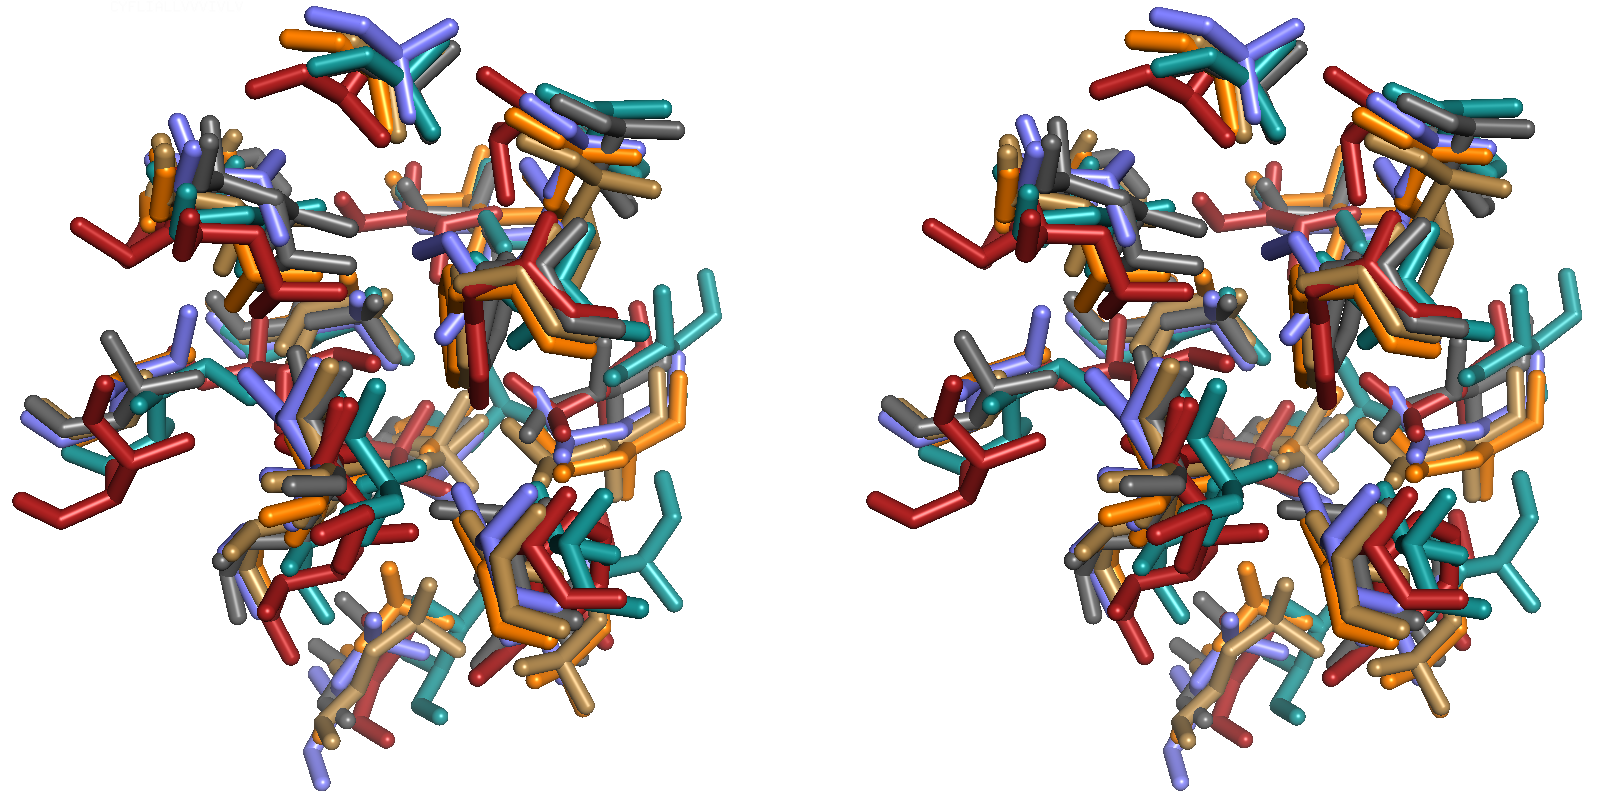
\includegraphics[width=17cm]{corePDZ.png} \\
     \end{tabular}
     \caption{le cœur PDZ sélectionné}
\label{graph:corePDZ}
   \end{figure}

    \clearpage

   \begin{figure}[t]
 \raggedleft{}
     \begin{tabular}{c}
       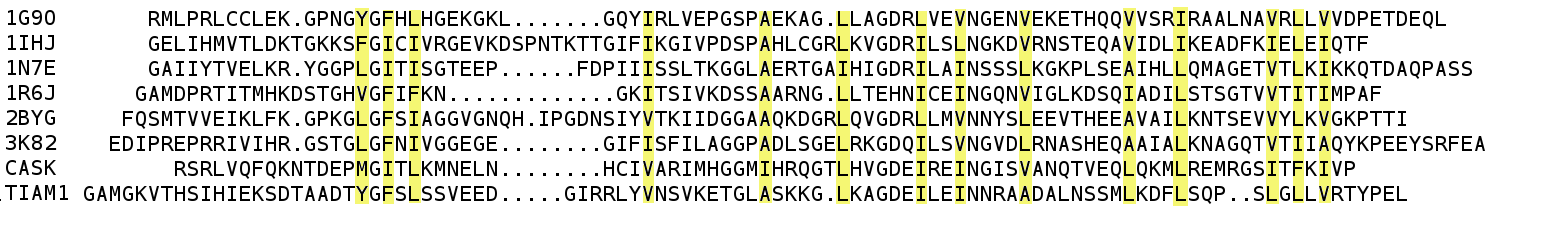
\includegraphics[width=18cm]{natives_alignees.png} \\
     \end{tabular}
     \caption{l'aligenement des séquences natives;le cœur PDZ sélectionné est en jaune.}
\label{graph:corePDZ}
   \end{figure}


    \clearpage
    \thispagestyle{empty}
   \begin{figure}[t]
     \centering
     \begin{tabular}{cc}
       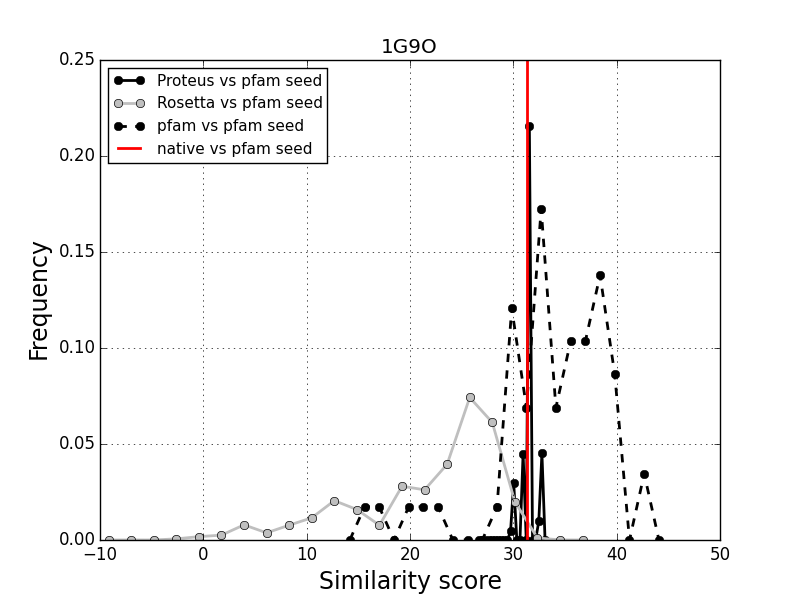
\includegraphics[width=8.4cm]{optGrad0/RP55/1G9O_core_simil.png} &
       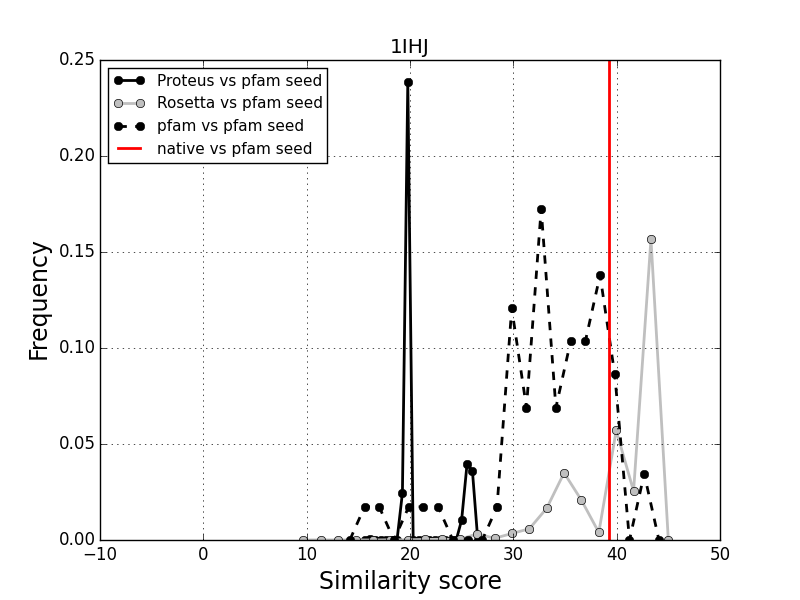
\includegraphics[width=8.4cm]{optGrad0/RP55/1IHJ_core_simil.png} \\
       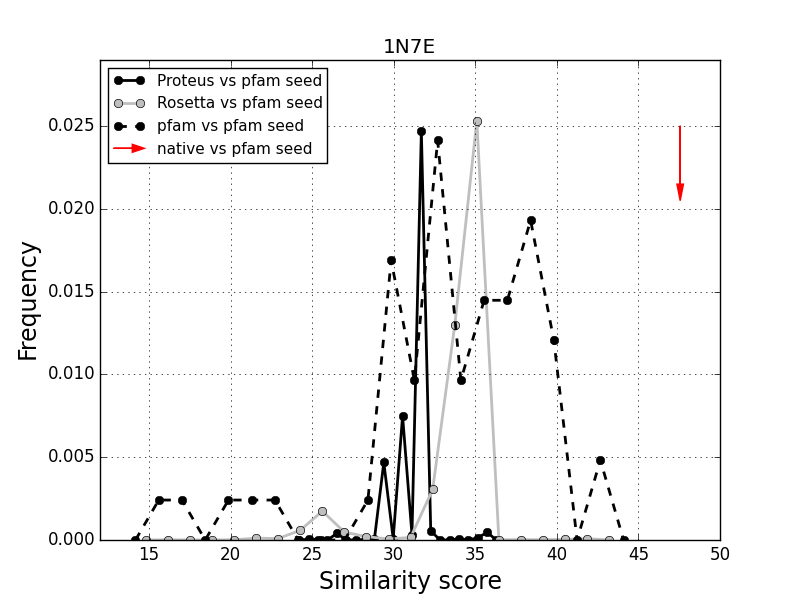
\includegraphics[width=8.4cm]{optGrad0/RP55/1N7E_core_simil.png} &
       \includegraphics[width=8.4cm]{optGrad0/RP55/1R6J_core_simil.png} \\
       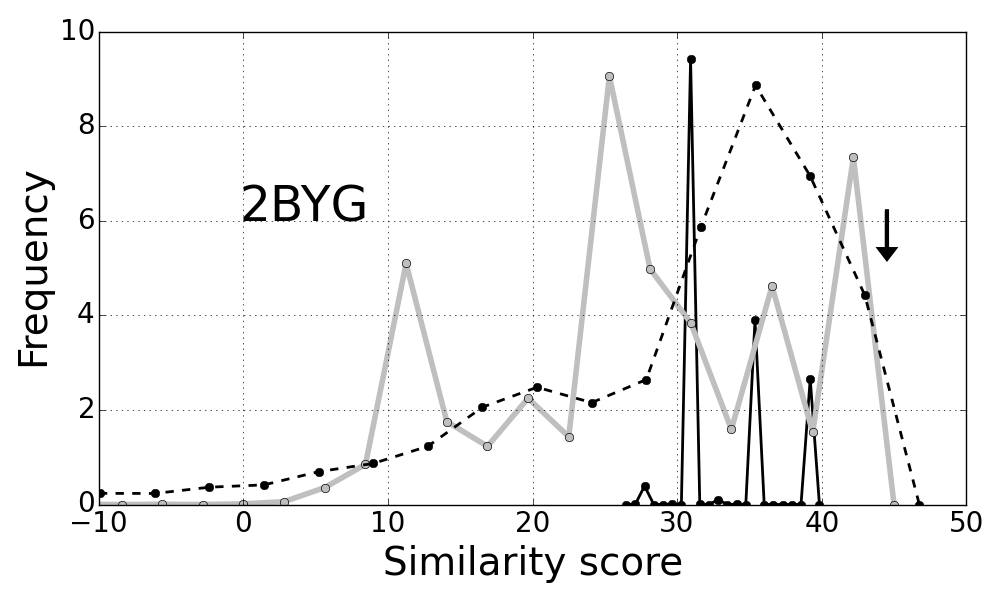
\includegraphics[width=8.4cm]{optGrad0/RP55/2BYG_core_simil.png} &
       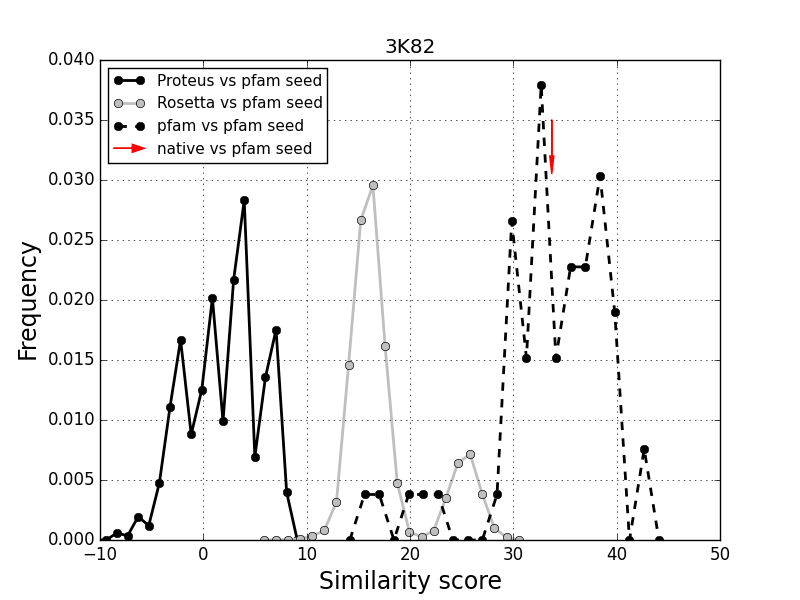
\includegraphics[width=8.4cm]{optGrad0/RP55/3K82_core_simil.png} \\
       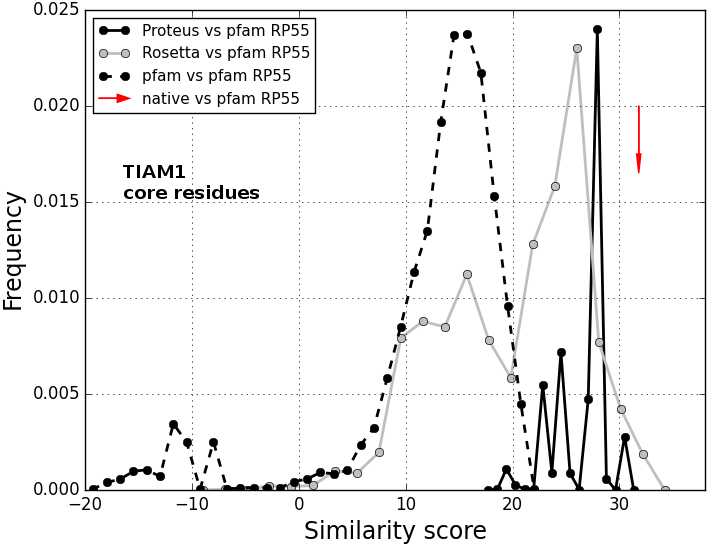
\includegraphics[width=8.4cm]{optGrad0/RP55/TIAM1_core_simil.png} &
       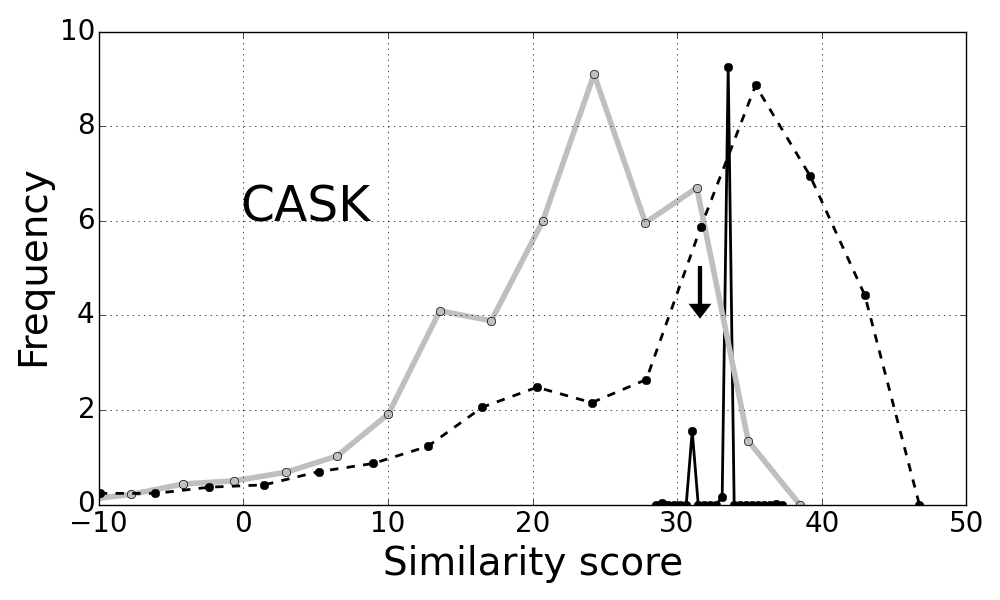
\includegraphics[width=8.4cm]{optGrad0/RP55/CASK_core_simil.png} \\ 
     \end{tabular}
%    \caption{Similarité des séquences Proteus(Enegie de référence sur 6 protéines) et Rosetta à l'alignement Pfam RP55, aux positions du cœur.}

\label{graph:Simil_Proteus_PDZ}
   \end{figure}

    \clearpage

    \begin{table}[!htbp]
      \centering

      \begin{tabular}{ccccccc}

        \toprule
        Protein & Proteus &  Proteus2 &  Proteus3 & Rosetta & Pfam seed \\
        \cmidrule{1-6}
        1G9O  & 1.40 & 1.42 & 1.47 & 1.45 & 3.15  \\
        1IHJ  & 1.38 & 1.46 & 1.51 & 1.55 & 3.06  \\
        1N7E  & 1.37 & 1.37 & 1.69 & 1.44 & 3.09  \\
        1R6J  & 1.39 & 1.44 & 1.53 & 1.43 & 3.03  \\
        2BYG  & 1.27 & 1.30 & 1.78 & 1.57 & 3.11  \\
        3K82  & 1.28 & 1.40 & 1.50 & 1.40 & 3.15  \\
        CASK  & 1.45 & 1.95 & 1.62 & 1.68 & 3.15  \\
        TIAM1 & 1.35 & 1.62 & 1.72 & 1.57 & 3.15  \\
        \bottomrule

      \end{tabular}      
      \caption{Moyenne de l'exponentiel de l'entropie sur les ensembles des positions des protéines}
\label{tab:Entropie_PDZ}      
    \end{table}

    \clearpage

    \begin{table}[!htbp]
      \centering

      \begin{tabular}{ccc}

        \toprule
        Sequences & Proteus & Rosetta \\
        \cmidrule{1-3}
        1G9O  & 1.38  & 1.45 \\
        1IHJ  & 1.37  & 1.55 \\
        1N7E  & 1.33  & 1.44 \\
        1R6J  & 1.39  & 1.43 \\
        2BYG  & 1.24  & 1.57 \\
        3K82  & 1.27  & 1.40 \\
        6prots & 2.42  & 2.88 \\
        TIAM1  & 1.55  & 1.57 \\
        CASK   & 1.22  & 1.69 \\

        \bottomrule

      \end{tabular}      
      \caption{Moyenne de l'exponentiel de l'entropie sur les ensembles des positions des protéines(énergies de référence optimisées sur six protéines)}
\label{tab:Entropie_PDZ}      
    \end{table}



    \begin{table}[!htbp]

\scalebox{0.85}{
      \begin{tabular}{ccccccccc}

        \toprule
        Protein & 1G9O & 1IHJ & 1N7E & 1R6J & 2BYG & 3K82 & CASK & TIAM1 \\
        \cmidrule{1-9}

        1G9O & 2e-66 (100)& 5e-10 (40)& 0.002 (25)& 3e-07 (25)& 2e-11 (35)& 1e-12 (30)& 5e-05 (25)& 9e-07(35)\\     
        1IHJ & 5e-10 (40) & 3e-68 (100)&  2e-07 (27)& no      & 2e-08 (27) & 9e-14 (46)& 4e-06 (35)& no    \\
        1N7E & 0.002 (25) & 2e-07 (27)&  3e-67 (100)& no       & 3e-14 (36) & 2e-10 (37)& 9e-12 (30)& 5e-05 (35)\\
        1R6J & 3e-07 (25) & no    &    no    & 1e-59 (100) &  no      & 1e-06 (32)& 0.007 (32)& no    \\
        2BYG & 2e-11 (35) & 2e-08 (27)&  3e-14 (37)& no      & 7e-71 (100) & 3e-15 (37)& 2e-07 (28)& 5e-05 (41)\\
        3K82 & 1e-12 (30) & 9e-14 (46)&  2e-10 (36)& 1e-06 (32)& 3e-15 (37) & 4e-70 (100)& 1e-07 (27)& 6e-04(33) \\
        Cask & 5e-05 (25) & 4e-06 (35)&  9e-12 (30)& 0.007 (32)& 2e-07 (28) & 1e-07 (27)& 7e-61 (100)& 5e-04(33) \\
        Tiam1 & 9e-07 (35)  &  no     &  5e-05 (35)& no      & 5e-05 (41) & 6e-04 (33)& 5e-04 (33)& 1e-68 (100)\\
        \bottomrule


      \end{tabular} 
}     
      \caption{E-value et pourcentage d'identité des alignements Blast croisés pour nos séquences PDZ. (no= pas de touche avec une E-value inférieure à 10)}
\label{tab:Xblast}      
    \end{table}



    \begin{table}[!htbp]
      \centering

      \begin{tabular}{ccccc}

        \toprule
        Sequences & Proteus & Rosetta & Proteus (inclus G et P) & Rosetta (inclus G et P)\\
        \cmidrule{1-5}
        1G9O  & 28 &  43 & 44 & 59 \\
        1IHJ  & 26 &  40 & 35 & 49 \\
        1N7E  & 33 &  48 & 50 & 65 \\
        1R6J  & 26 &  46 & 38 & 58 \\
        2BYG  & 28 &  46 & 42 & 61 \\
        3K82  & 36 &  52 & 54 & 70 \\
        TIAM1 & 18 &  25 & 28 & 30 \\
        CASK  & 17 &  28 & 28 &  39 \\

        \bottomrule

      \end{tabular}      
      \caption{Pourcentage d'identité moyen à la séquence native}
\label{tab:Entropie_PDZ}      
    \end{table}



\begin{table}[h]
  \raggedleft{}
  
  \begin{tabular}{cccccc}
    
    \toprule
    Protein & Match/seq & Superfamily & Superfamily & Family & Family \\
            & size      & Evalue      & success     & Evalue & success\\
    \cmidrule{1-6}
    1G9O  & 78/91 & 2.5e-3  & 10000 & 3.0e-3 & 10000 \\
    1IHJ  & 86/94 & 5.6e-7  & 10000 & 2.3e-3 & 10000 \\
    1N7E  & 81/95 & 1.1e-6  & 10000 & 2.4e-3 & 10000 \\
    1R6J  & 41/82 & 1.5     &  1350 & 2.6e-2 &  1350 \\
    2BYG  & 77/97 & 1.0e-2  & 10000 & 2.3e-3 & 10000 \\
    3K82  & 86/97 & 4.0e-16 & 10000 & 2.7e-3 & 10000 \\
    \cmidrule{1-6}
    CASK  & 72/83 & 2.3e-4  & 10000 & 1.5e-2 & 10000 \\
    TIAM1 & 43/94 & 1.28    & 442   & 4.0e-2 & 374 \\
    \cmidrule{1-6}
    1R6J-B & 70/82 & 1.4e-3    & 6664   & 4.0e-3 & 6664 \\
    \bottomrule        
  \end{tabular}   
  \caption{Résultats Superfamily pour les séquences Proteus avec le nouveau test Monte Carlo et énergies de référence optimisées sur l'ensemble réduit à six protéines}   
  \label{tab:superfamily_Old_MCtest}       
\end{table}




    \clearpage


   \begin{figure}[t]
     \centering
     \begin{tabular}{c}
       \includegraphics[width=17cm]{result/1G9O.png} \\
     \end{tabular}
     \caption{Sélection de séquences proteus 1G9O }
\label{result:1G9O}
   \end{figure}

   \begin{figure}[t]
     \centering
     \begin{tabular}{c}
       \includegraphics[width=17cm]{result/1IHJ.png} \\
     \end{tabular}
     \caption{Sélection de séquences proteus 1IHJ }
\label{result:1IHJ}
   \end{figure}

    \clearpage
   \begin{figure}[t]
     \centering
     \begin{tabular}{c}
       \includegraphics[width=17cm]{result/1N7E.png} \\
     \end{tabular}
     \caption{Sélection de séquences proteus 1N7E }
\label{result:1N7E}
   \end{figure}

   \begin{figure}[t]
     \centering
     \begin{tabular}{c}
       \includegraphics[width=17cm]{result/1R6J.png} \\
     \end{tabular}
     \caption{Sélection de séquences proteus 1R6J }
\label{result:1R6J}
   \end{figure}

    \clearpage

   \begin{figure}[t]
     \centering
     \begin{tabular}{c}
       \includegraphics[width=17cm]{result/2BYG.png} \\
     \end{tabular}
     \caption{Sélection de séquences proteus 2BYG }
\label{result:2BYG}
   \end{figure}

   \begin{figure}[t]
     \centering
     \begin{tabular}{c}
       \includegraphics[width=17cm]{result/3K82.png} \\
     \end{tabular}
     \caption{Sélection de séquences proteus 3K82 }
\label{result:3K82}
   \end{figure}

    \clearpage

   \begin{figure}[t]
     \centering
     \begin{tabular}{c}
       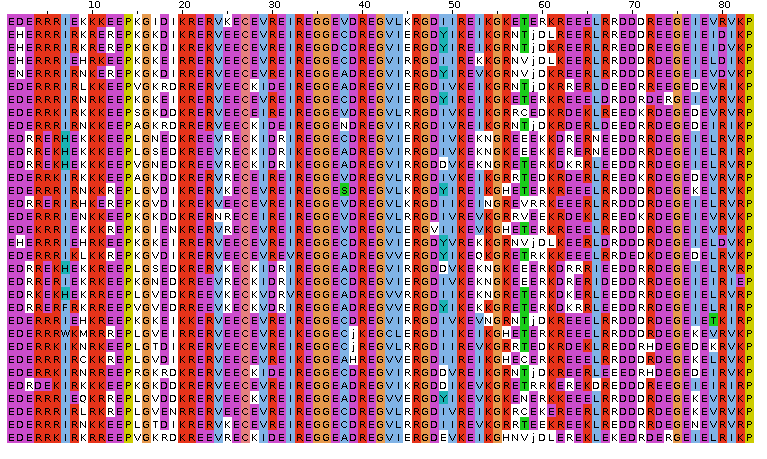
\includegraphics[width=17cm]{result/CASK.png} \\
     \end{tabular}
     \caption{Sélection de séquences proteus CASK }
\label{result:CASK}
   \end{figure}

   \begin{figure}[t]
     \centering
     \begin{tabular}{c}
       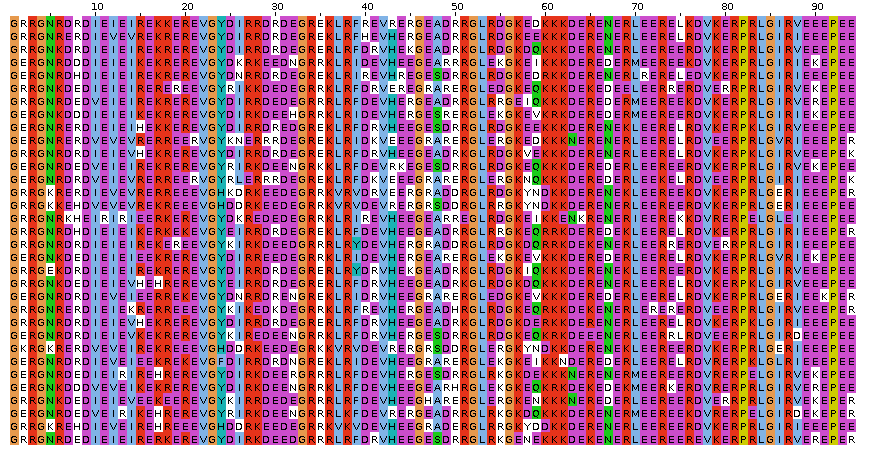
\includegraphics[width=17cm]{result/TIAM1.png} \\
     \end{tabular}
     \caption{Sélection de séquences proteus TIAM1 }
\label{result:TIAM1}
   \end{figure}

    \clearpage


   \begin{figure}[t]
     \centering
     \begin{tabular}{c}
       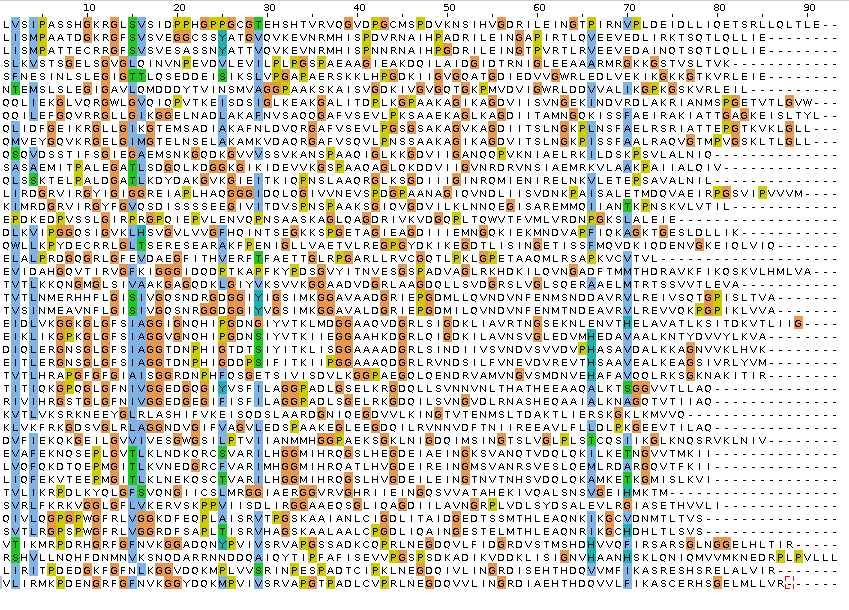
\includegraphics[width=17cm]{result/PDZ.png} \\
     \end{tabular}
     \caption{Les séquences de l'alignement PDZ seed de Pfam}
\label{result:PDZ_seed}
   \end{figure}

    \clearpage
\begin{landscape}

   \begin{figure}[t]
     \centering
     \begin{tabular}{c}
       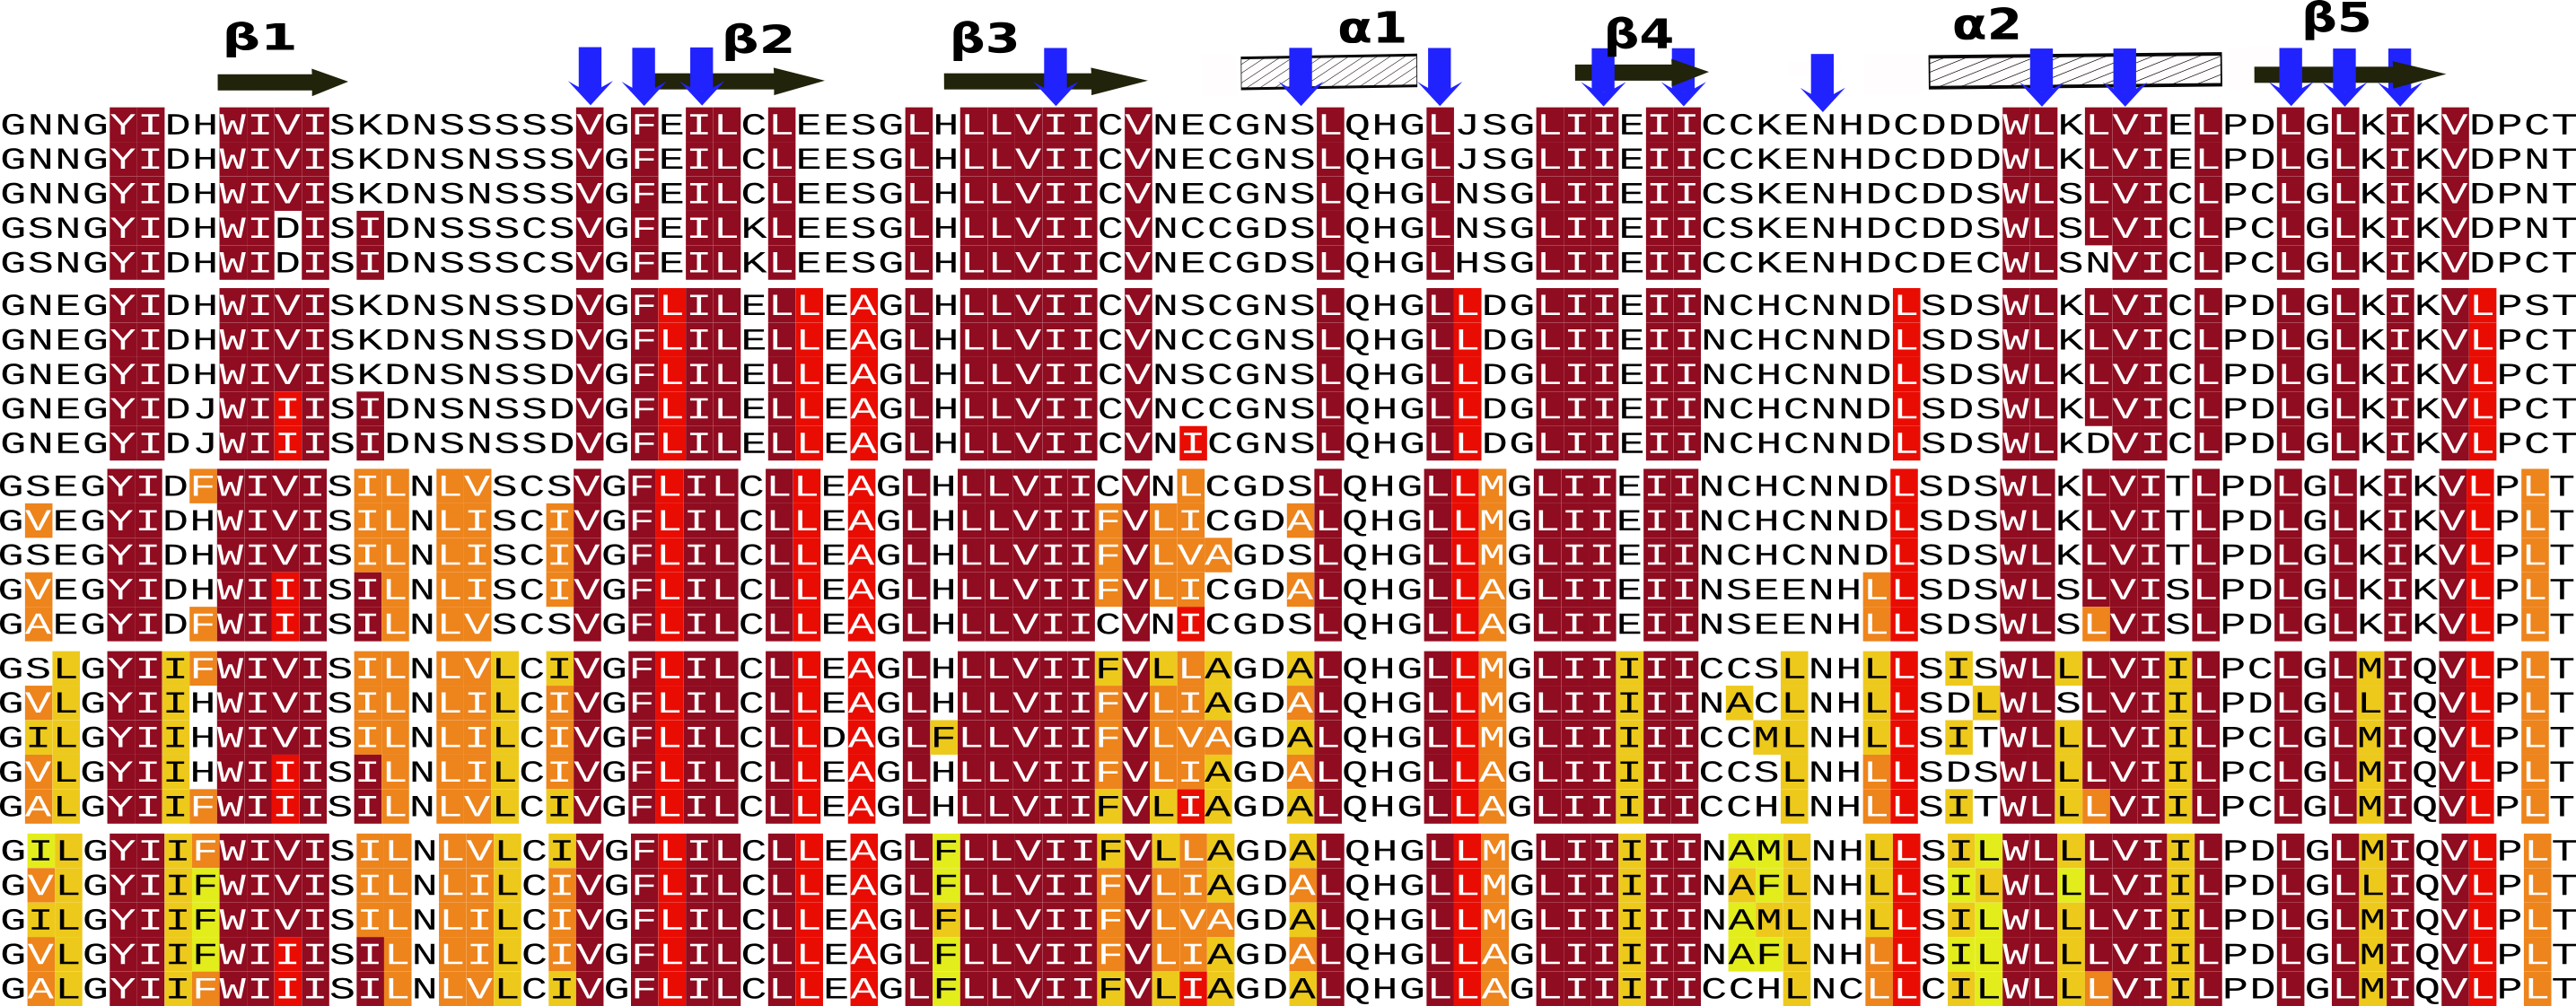
\includegraphics[width=18cm]{boost_hydro/modelA/alignTIAM1.png} \\
     \end{tabular}
%     \caption{Séquences Tiam1 obtenues avec un delta des énergies de références à -0.4,-0.2,0,0.2 et 0.4. Les hydrophobes sont représentés par un dégradé allant du rouge foncé au jaune clair.}
\label{result:PDZ_seed}
   \end{figure}

   \begin{figure}[t]
     \centering
     \begin{tabular}{c}
       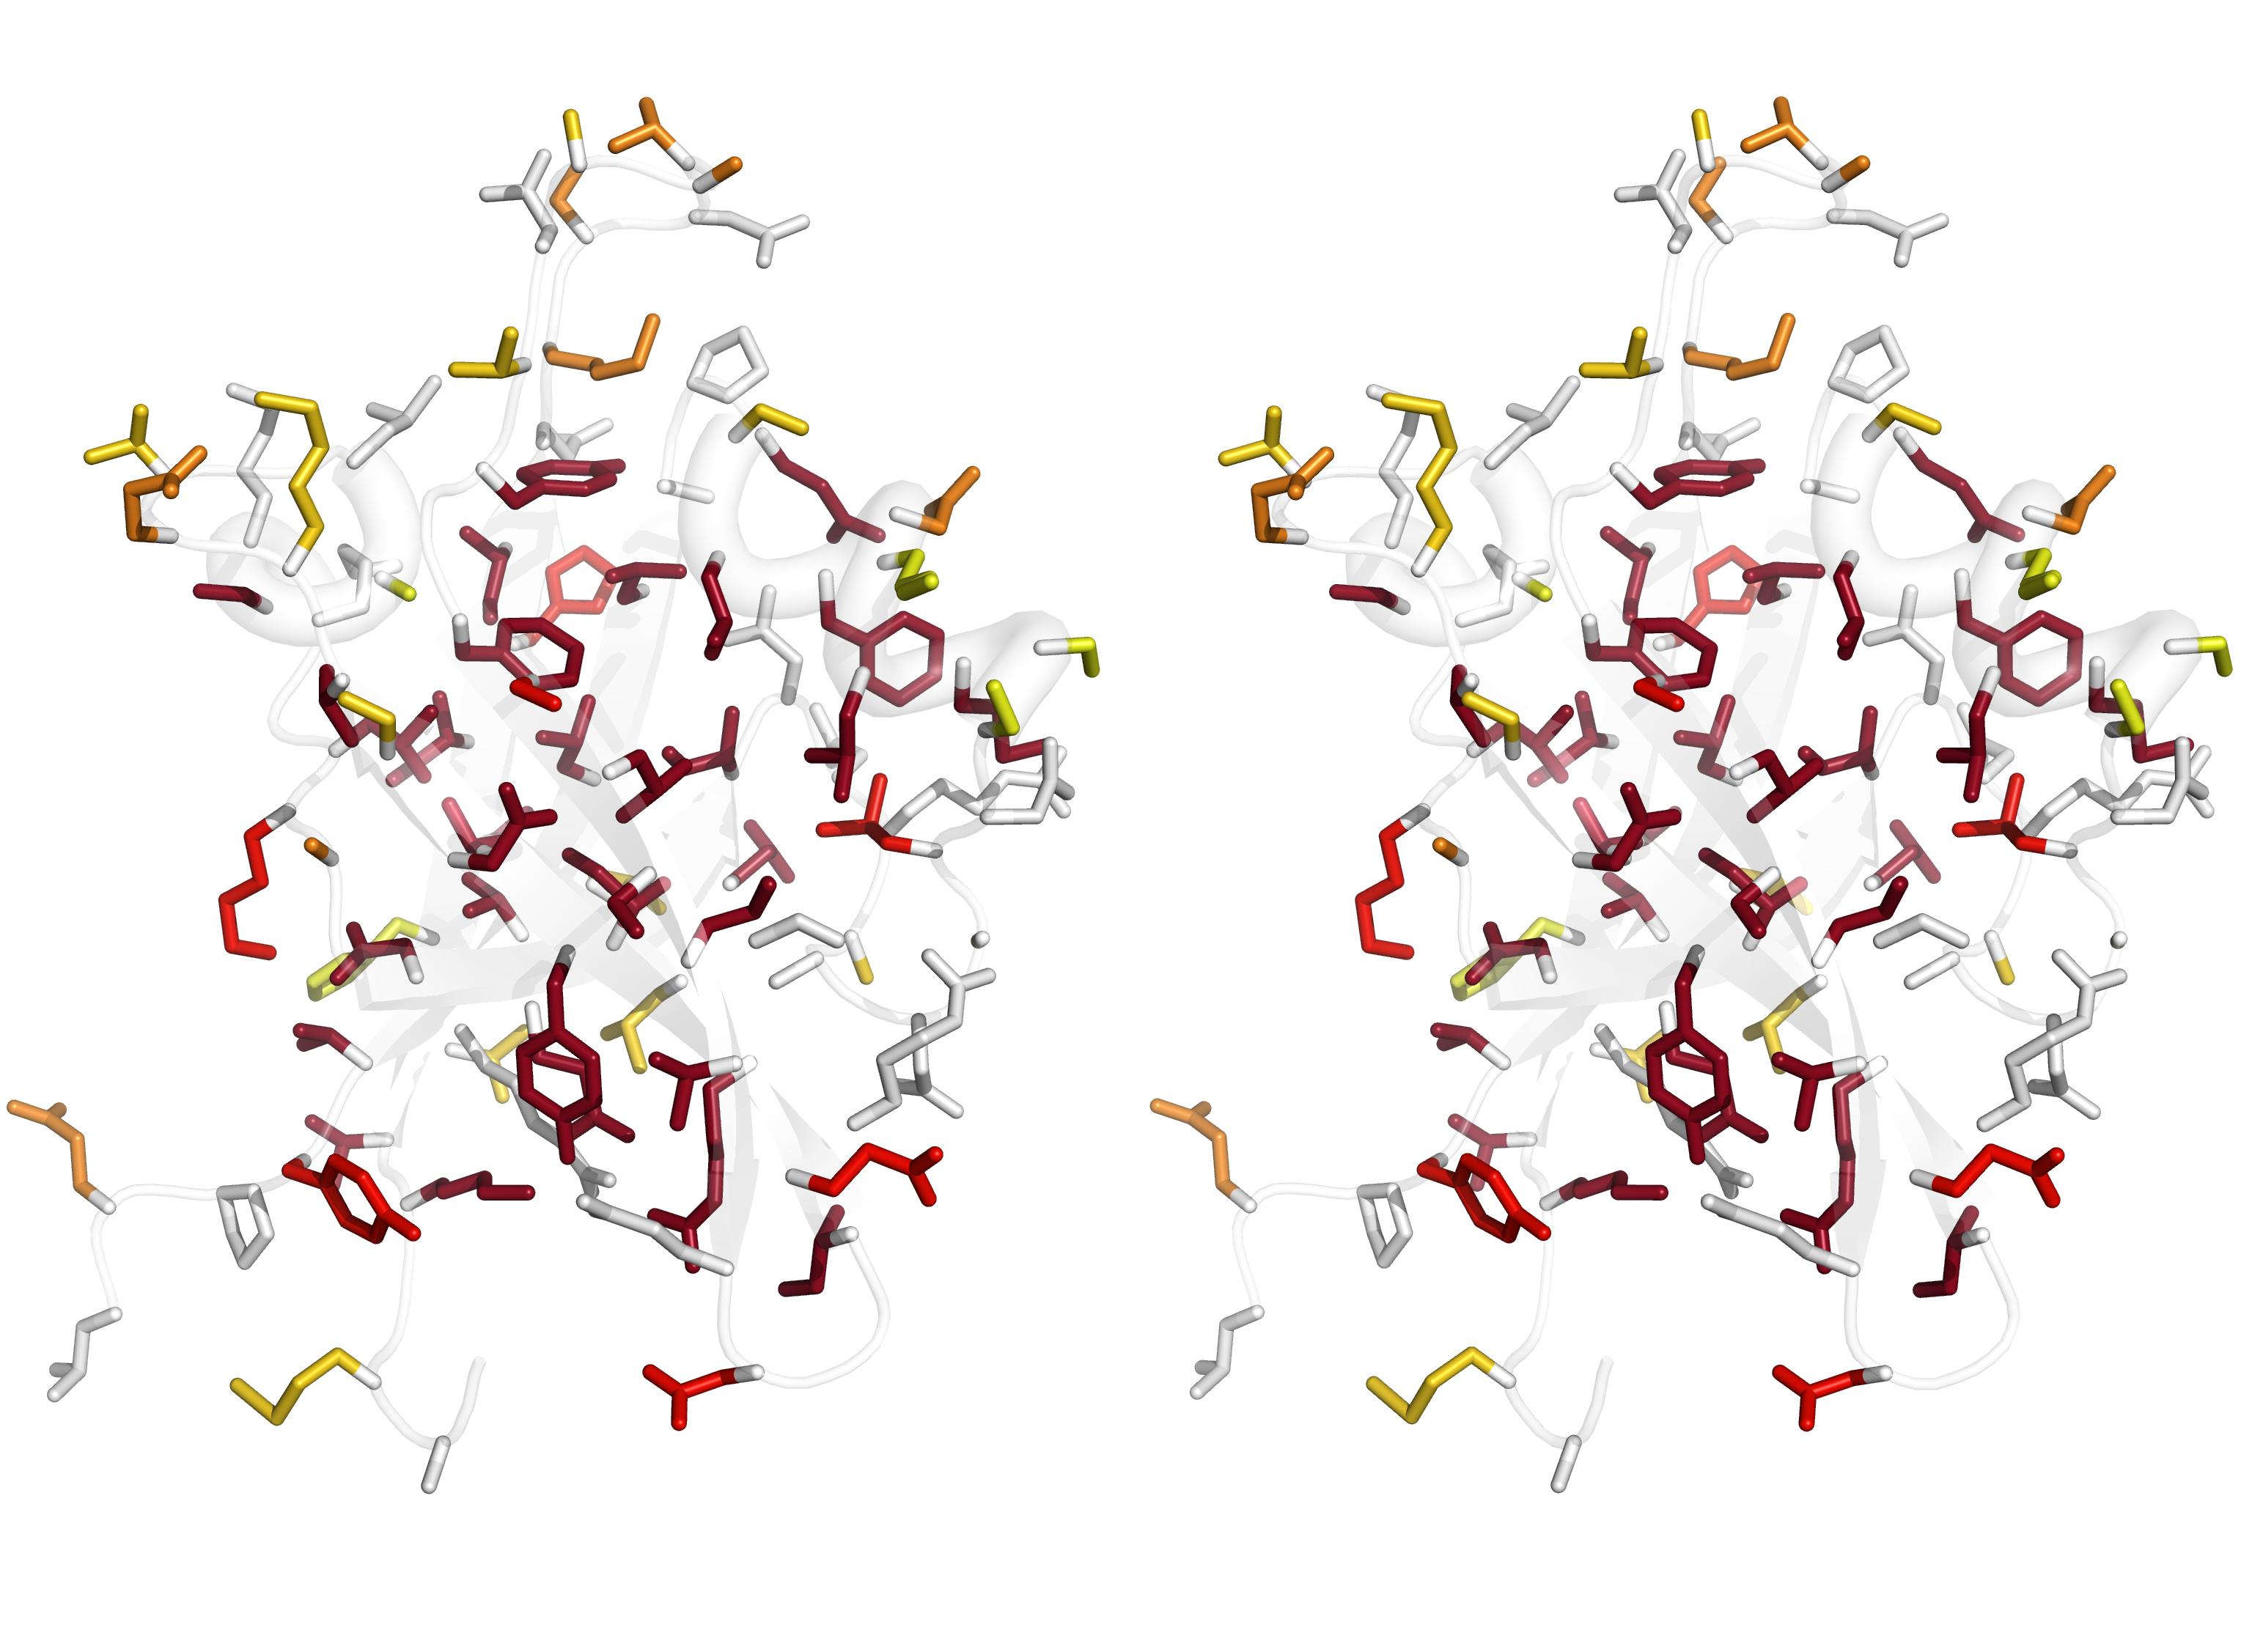
\includegraphics[width=9cm]{boost_hydro/modelA/structureTIAM1.png} \\
     \end{tabular}

     \caption{\small Séquences Tiam1 obtenues avec un delta des énergies de références à -0.4,-0.2,0,0.2 et 0.4 et la struture native.Les hydrophobes pour des deltas de -0.4,-0.2,0,0.2 et 0.4 sont représentés par un dégradé allant du rouge foncé au jaune clair.}

\label{result:PDZ_seed}
   \end{figure}

\end{landscape}


\clearpage
\thispagestyle{empty}
%\setcounter{page}{0}
\begin{landscape}

   \begin{figure}[t]
     \centering
     \begin{tabular}{l}
       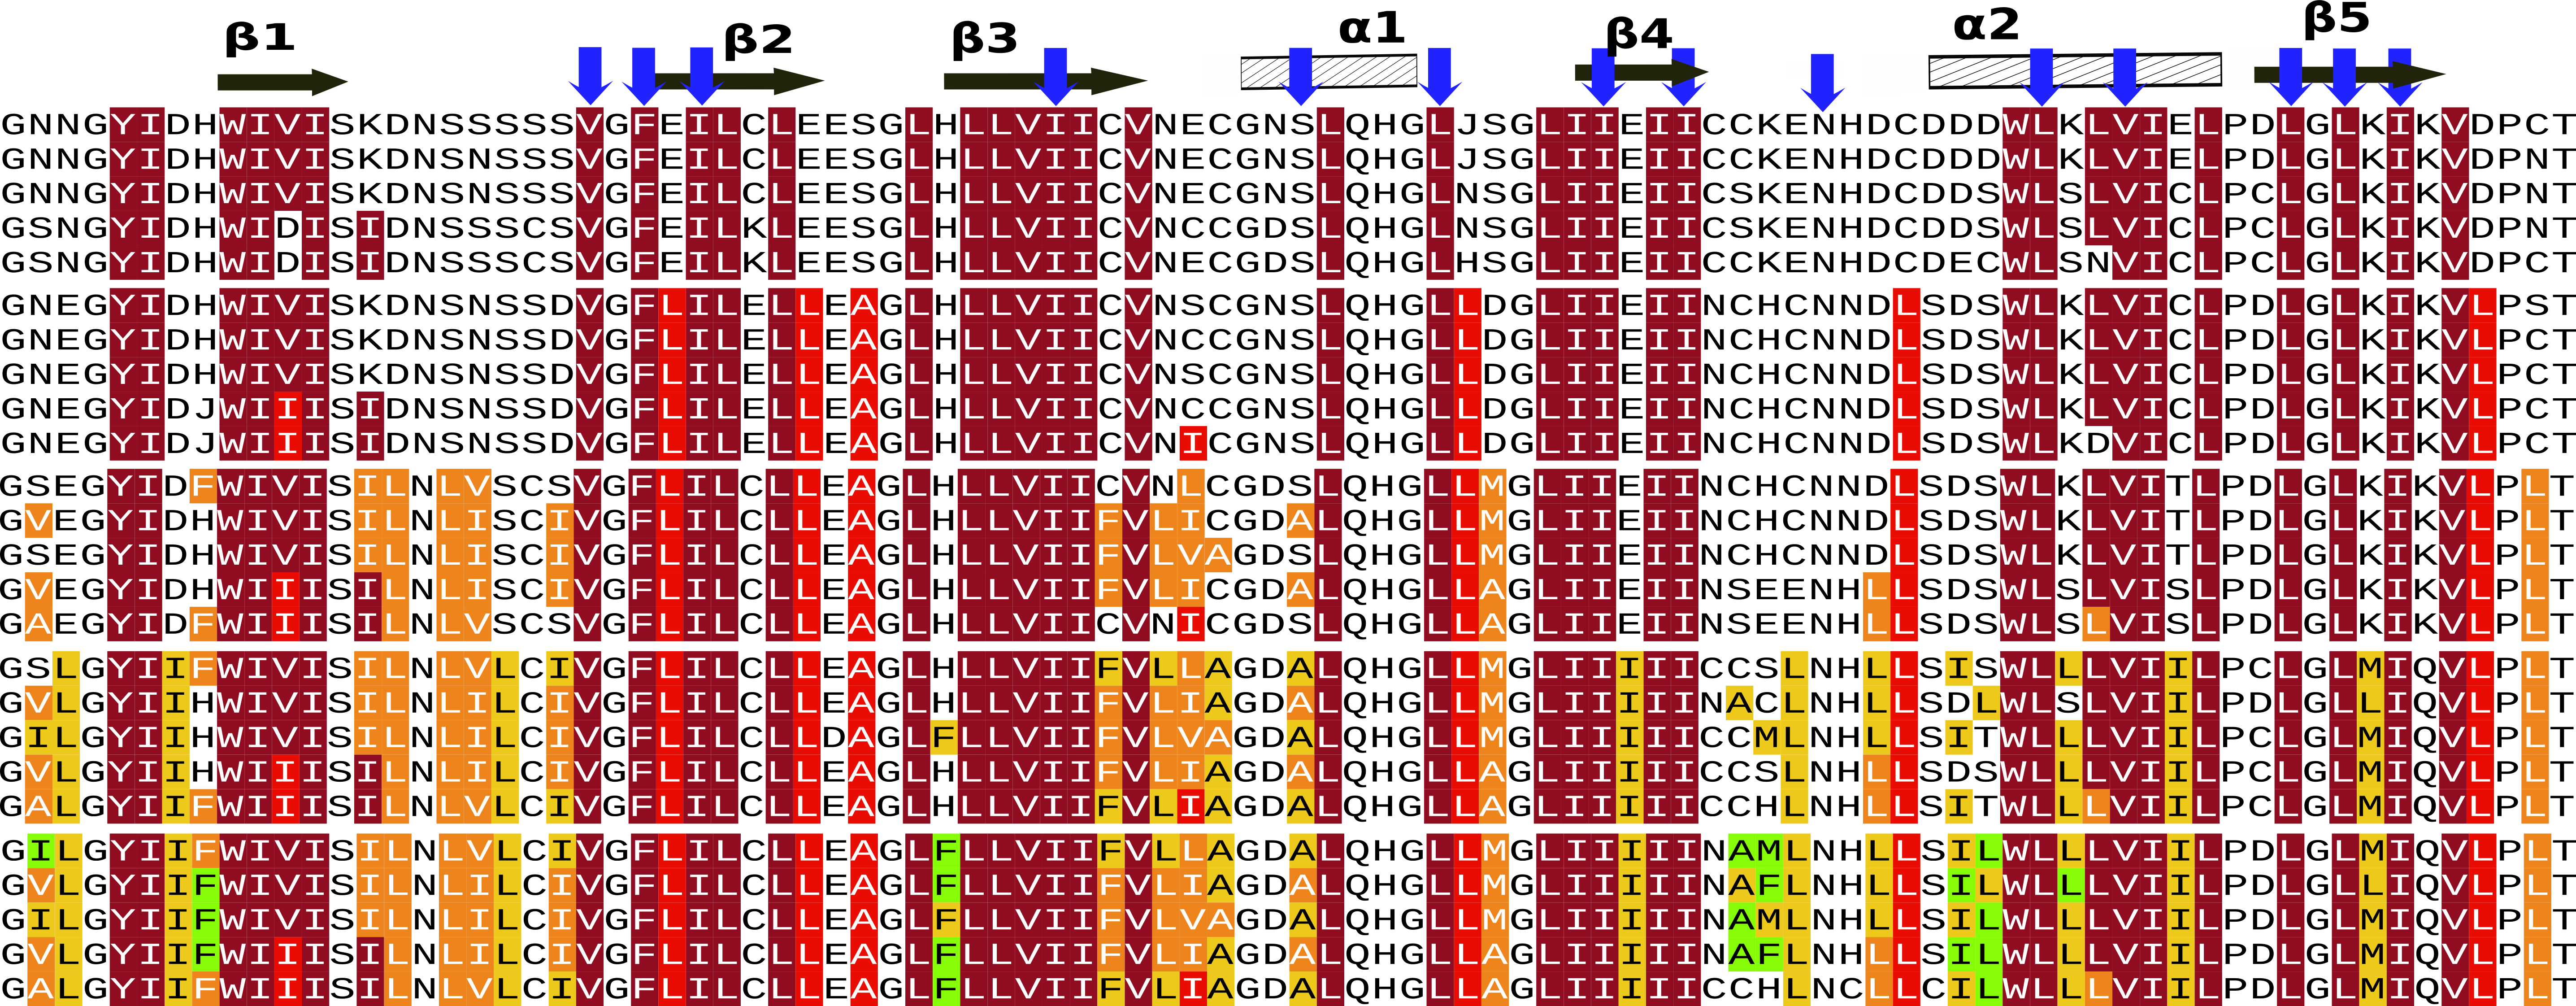
\includegraphics[width=18cm]{boost_hydro/modelA/alignTIAM1_V2.png} \\
       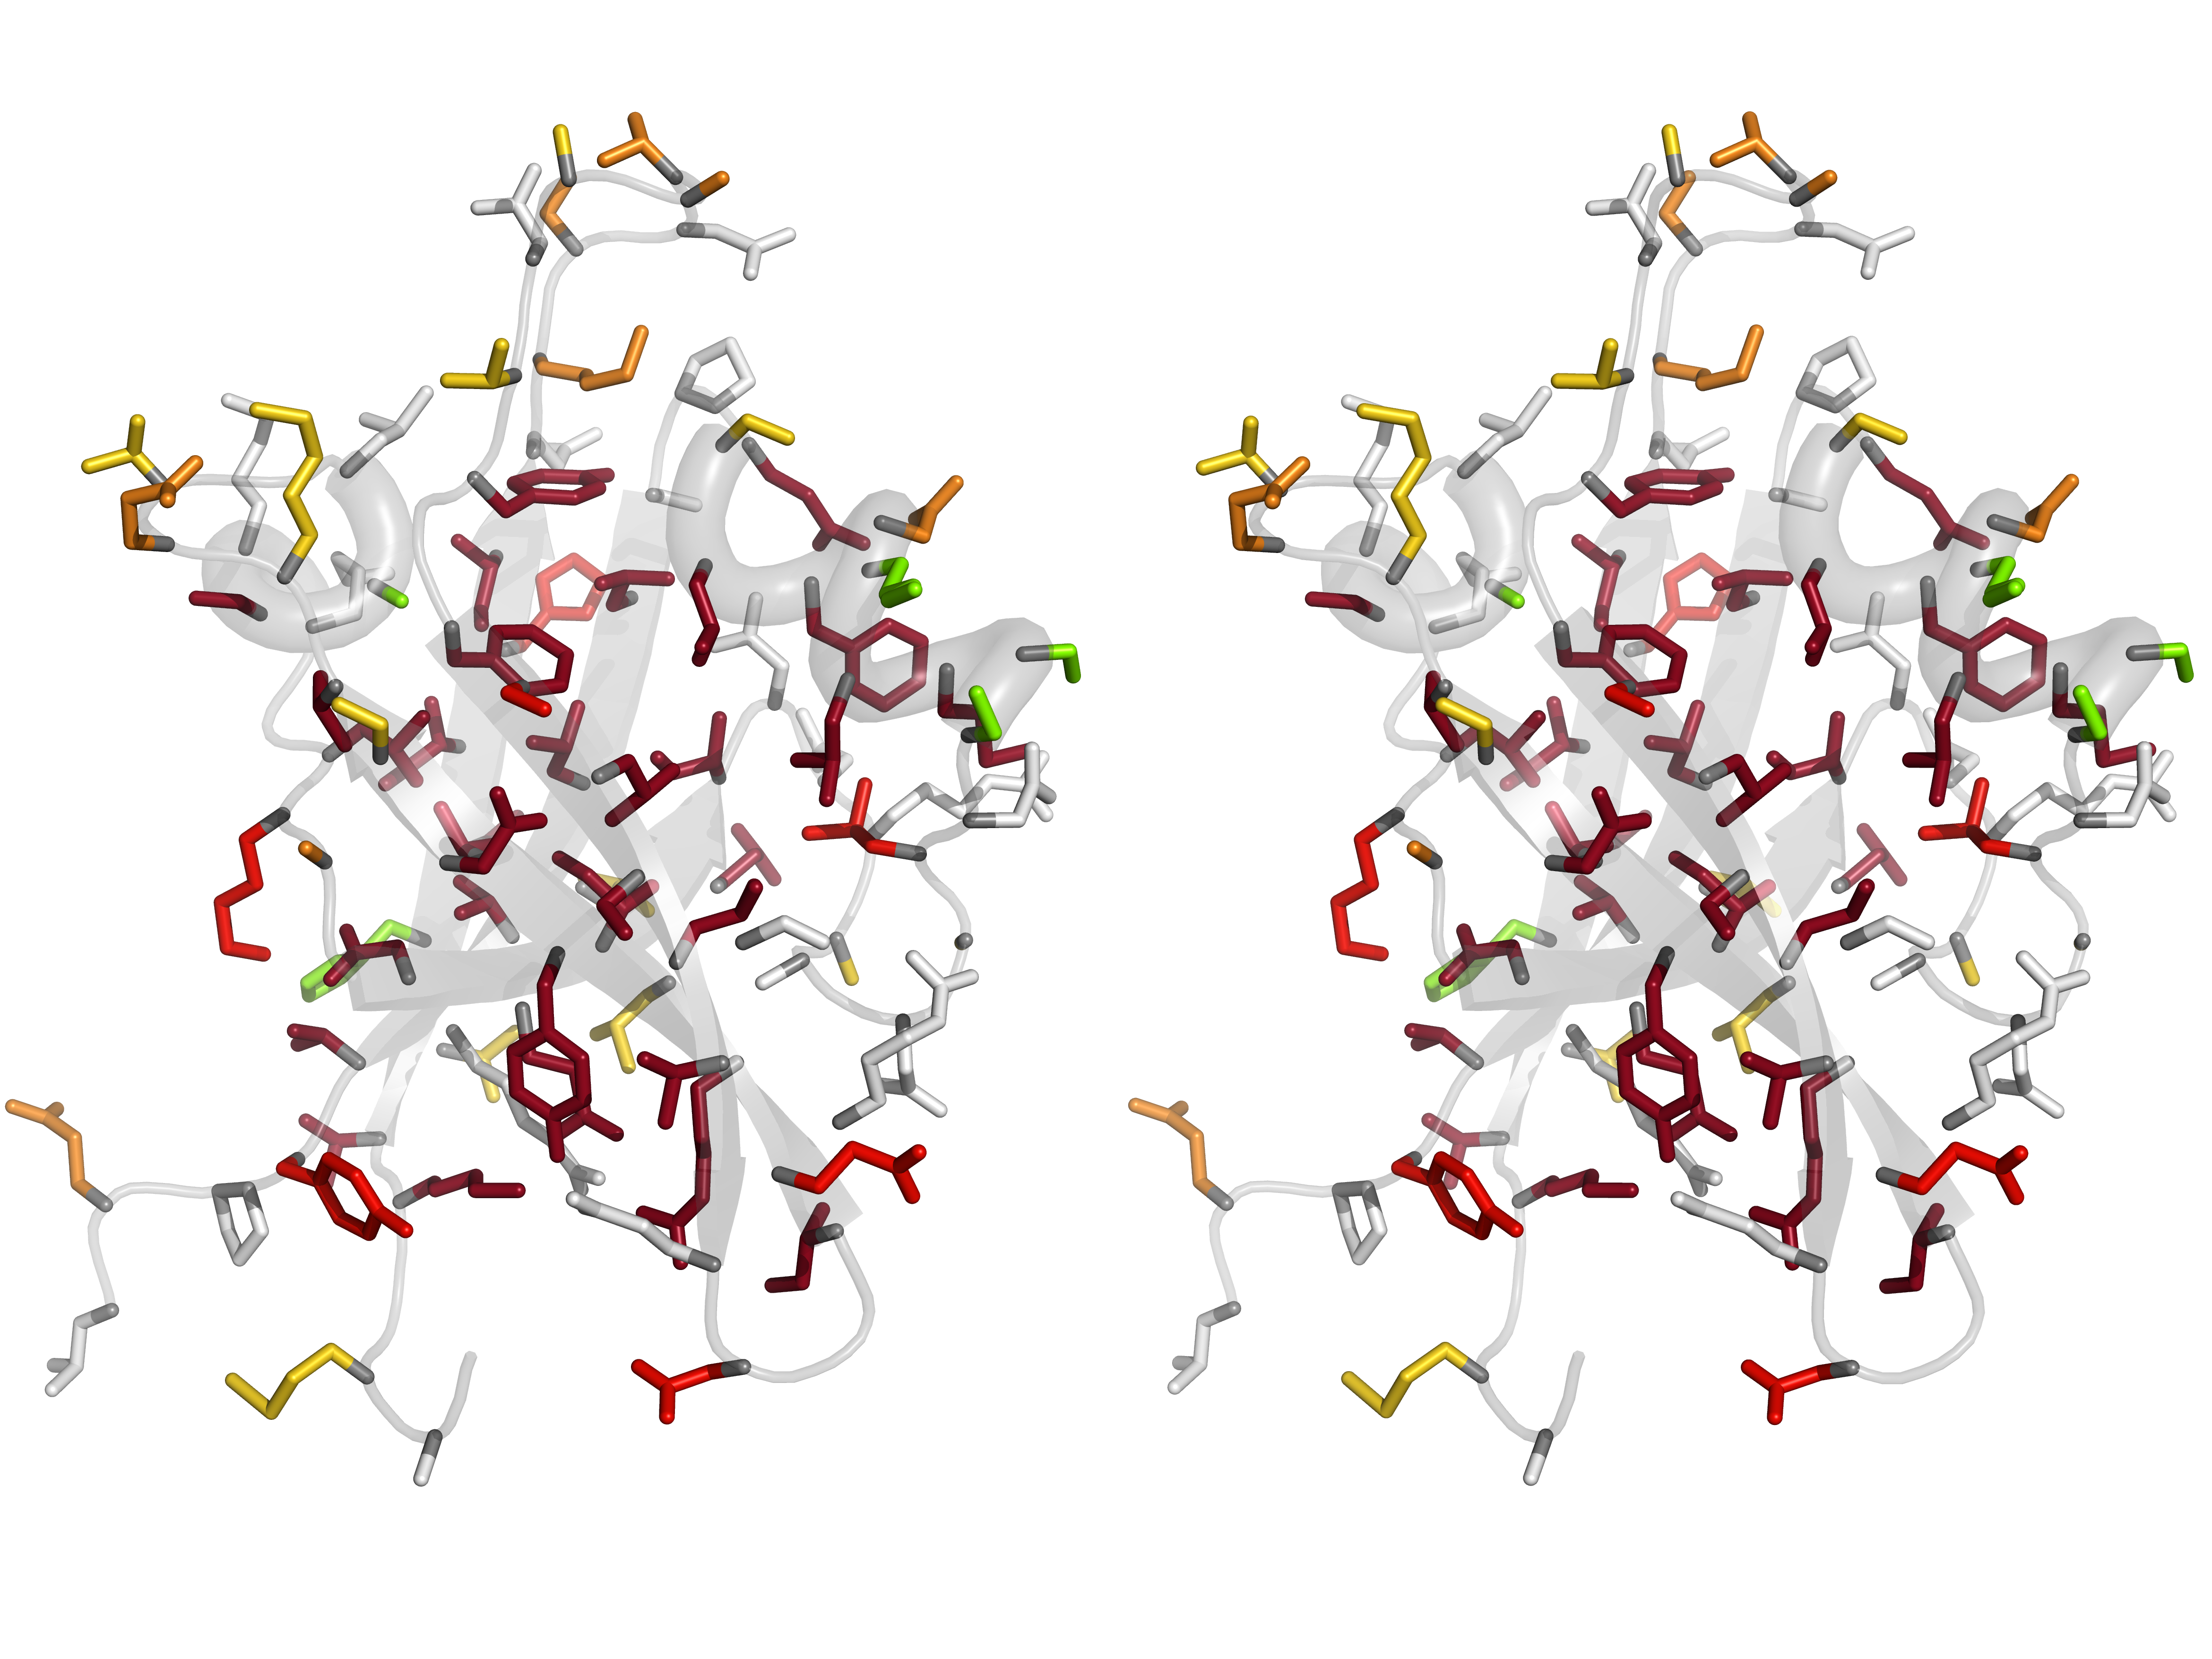
\includegraphics[width=11cm]{boost_hydro/modelA/structureTIAM1_V2.png} \\
     \end{tabular}
%     \caption{Séquences Tiam1 obtenues avec un delta des énergies de références à -0.4,-0.2,0,0.2 et 0.4. Les hydrophobes sont représentés par un dégradé allant du rouge foncé au jaune clair.}
\label{result:PDZ_seed}
   \end{figure}
%     \caption{\small Séquences Tiam1 obtenues avec un delta des énergies de références à -0.4,-0.2,0,0.2 et 0.4 et la struture native.Les hydrophobes pour des deltas de -0.4,-0.2,0,0.2 et 0.4 sont représentés par un dégradé allant du rouge foncé au jaune clair.}

\label{result:PDZ_seed}
   \end{figure}

\end{landscape}


    \clearpage

\begin{landscape}

   \begin{figure}[t]
     \centering
     \begin{tabular}{c}
       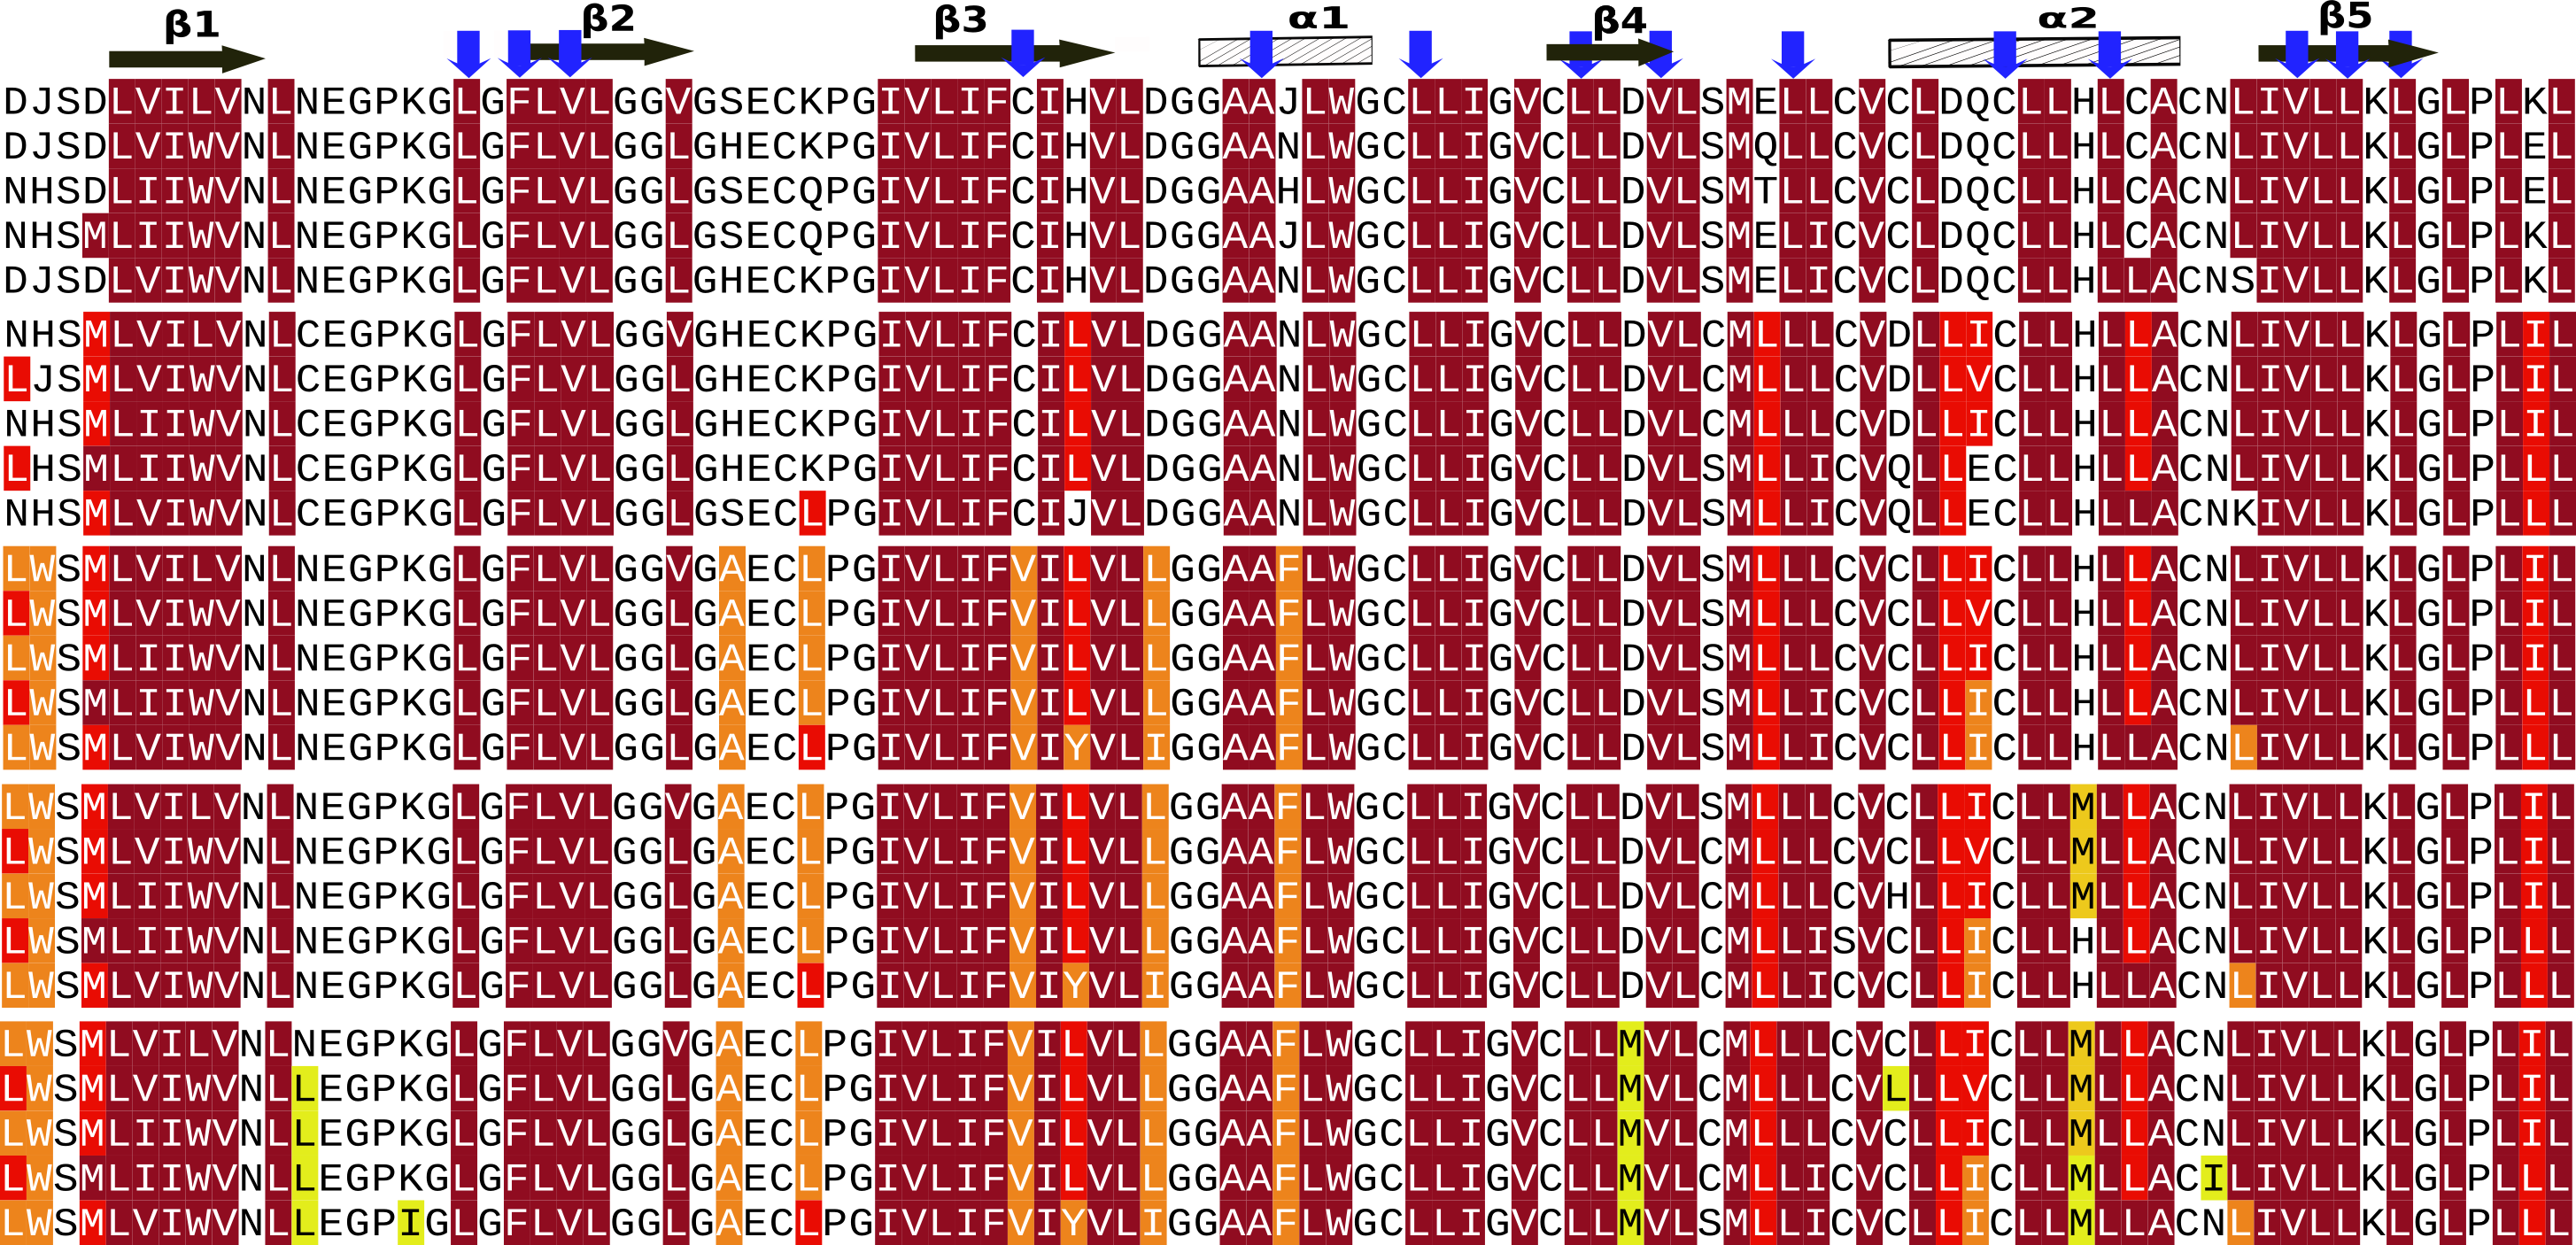
\includegraphics[width=14cm]{boost_hydro/modelA/align2BYG.png} \\
     \end{tabular}
%     \caption{Séquences Tiam1 obtenues avec un delta des énergies de références à -0.4,-0.2,0,0.2 et 0.4. Les hydrophobes sont représentés par un dégradé allant du rouge foncé au jaune clair.}
\label{result:PDZ_seed}
   \end{figure}

   \begin{figure}[t]
     \centering
     \begin{tabular}{c}
       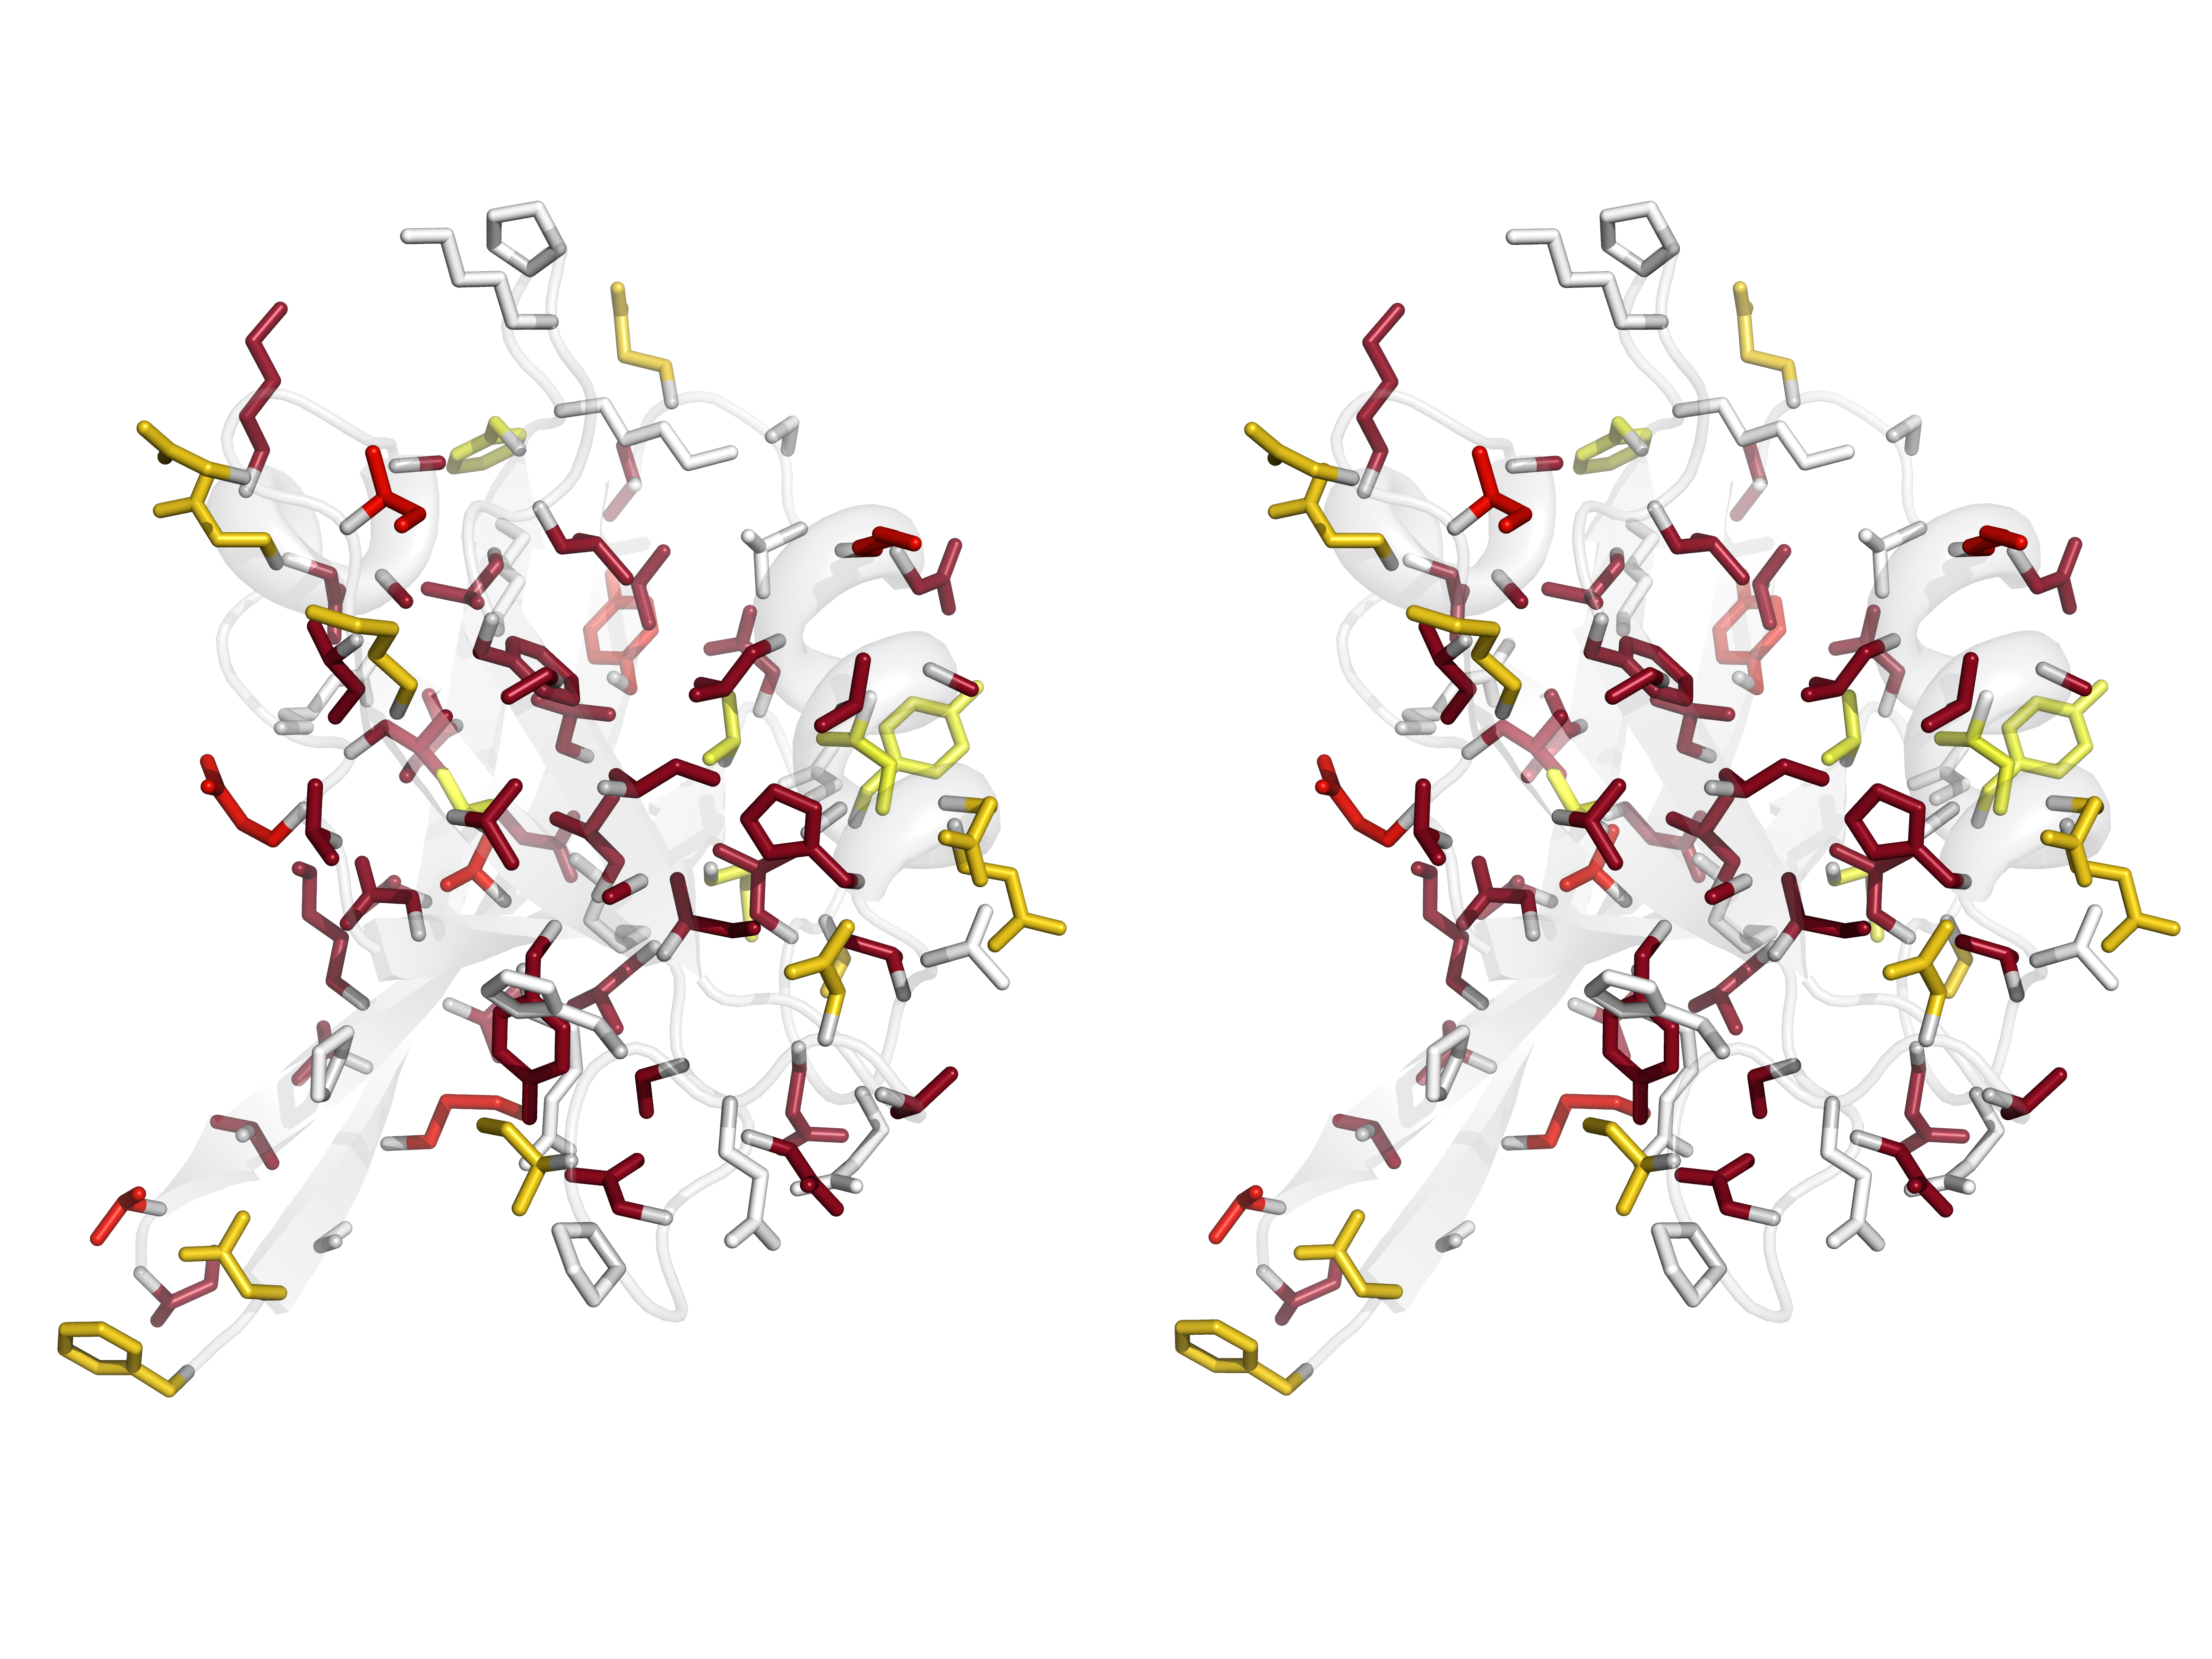
\includegraphics[width=9cm]{boost_hydro/modelA/structure2BYG.png} \\
     \end{tabular}

     \caption{\small Séquences 2BYG.}

\label{result:PDZ_seed}
   \end{figure}

\end{landscape}


   \clearpage

\begin{landscape}

   \begin{figure}[t]
     \centering
     \begin{tabular}{c}
       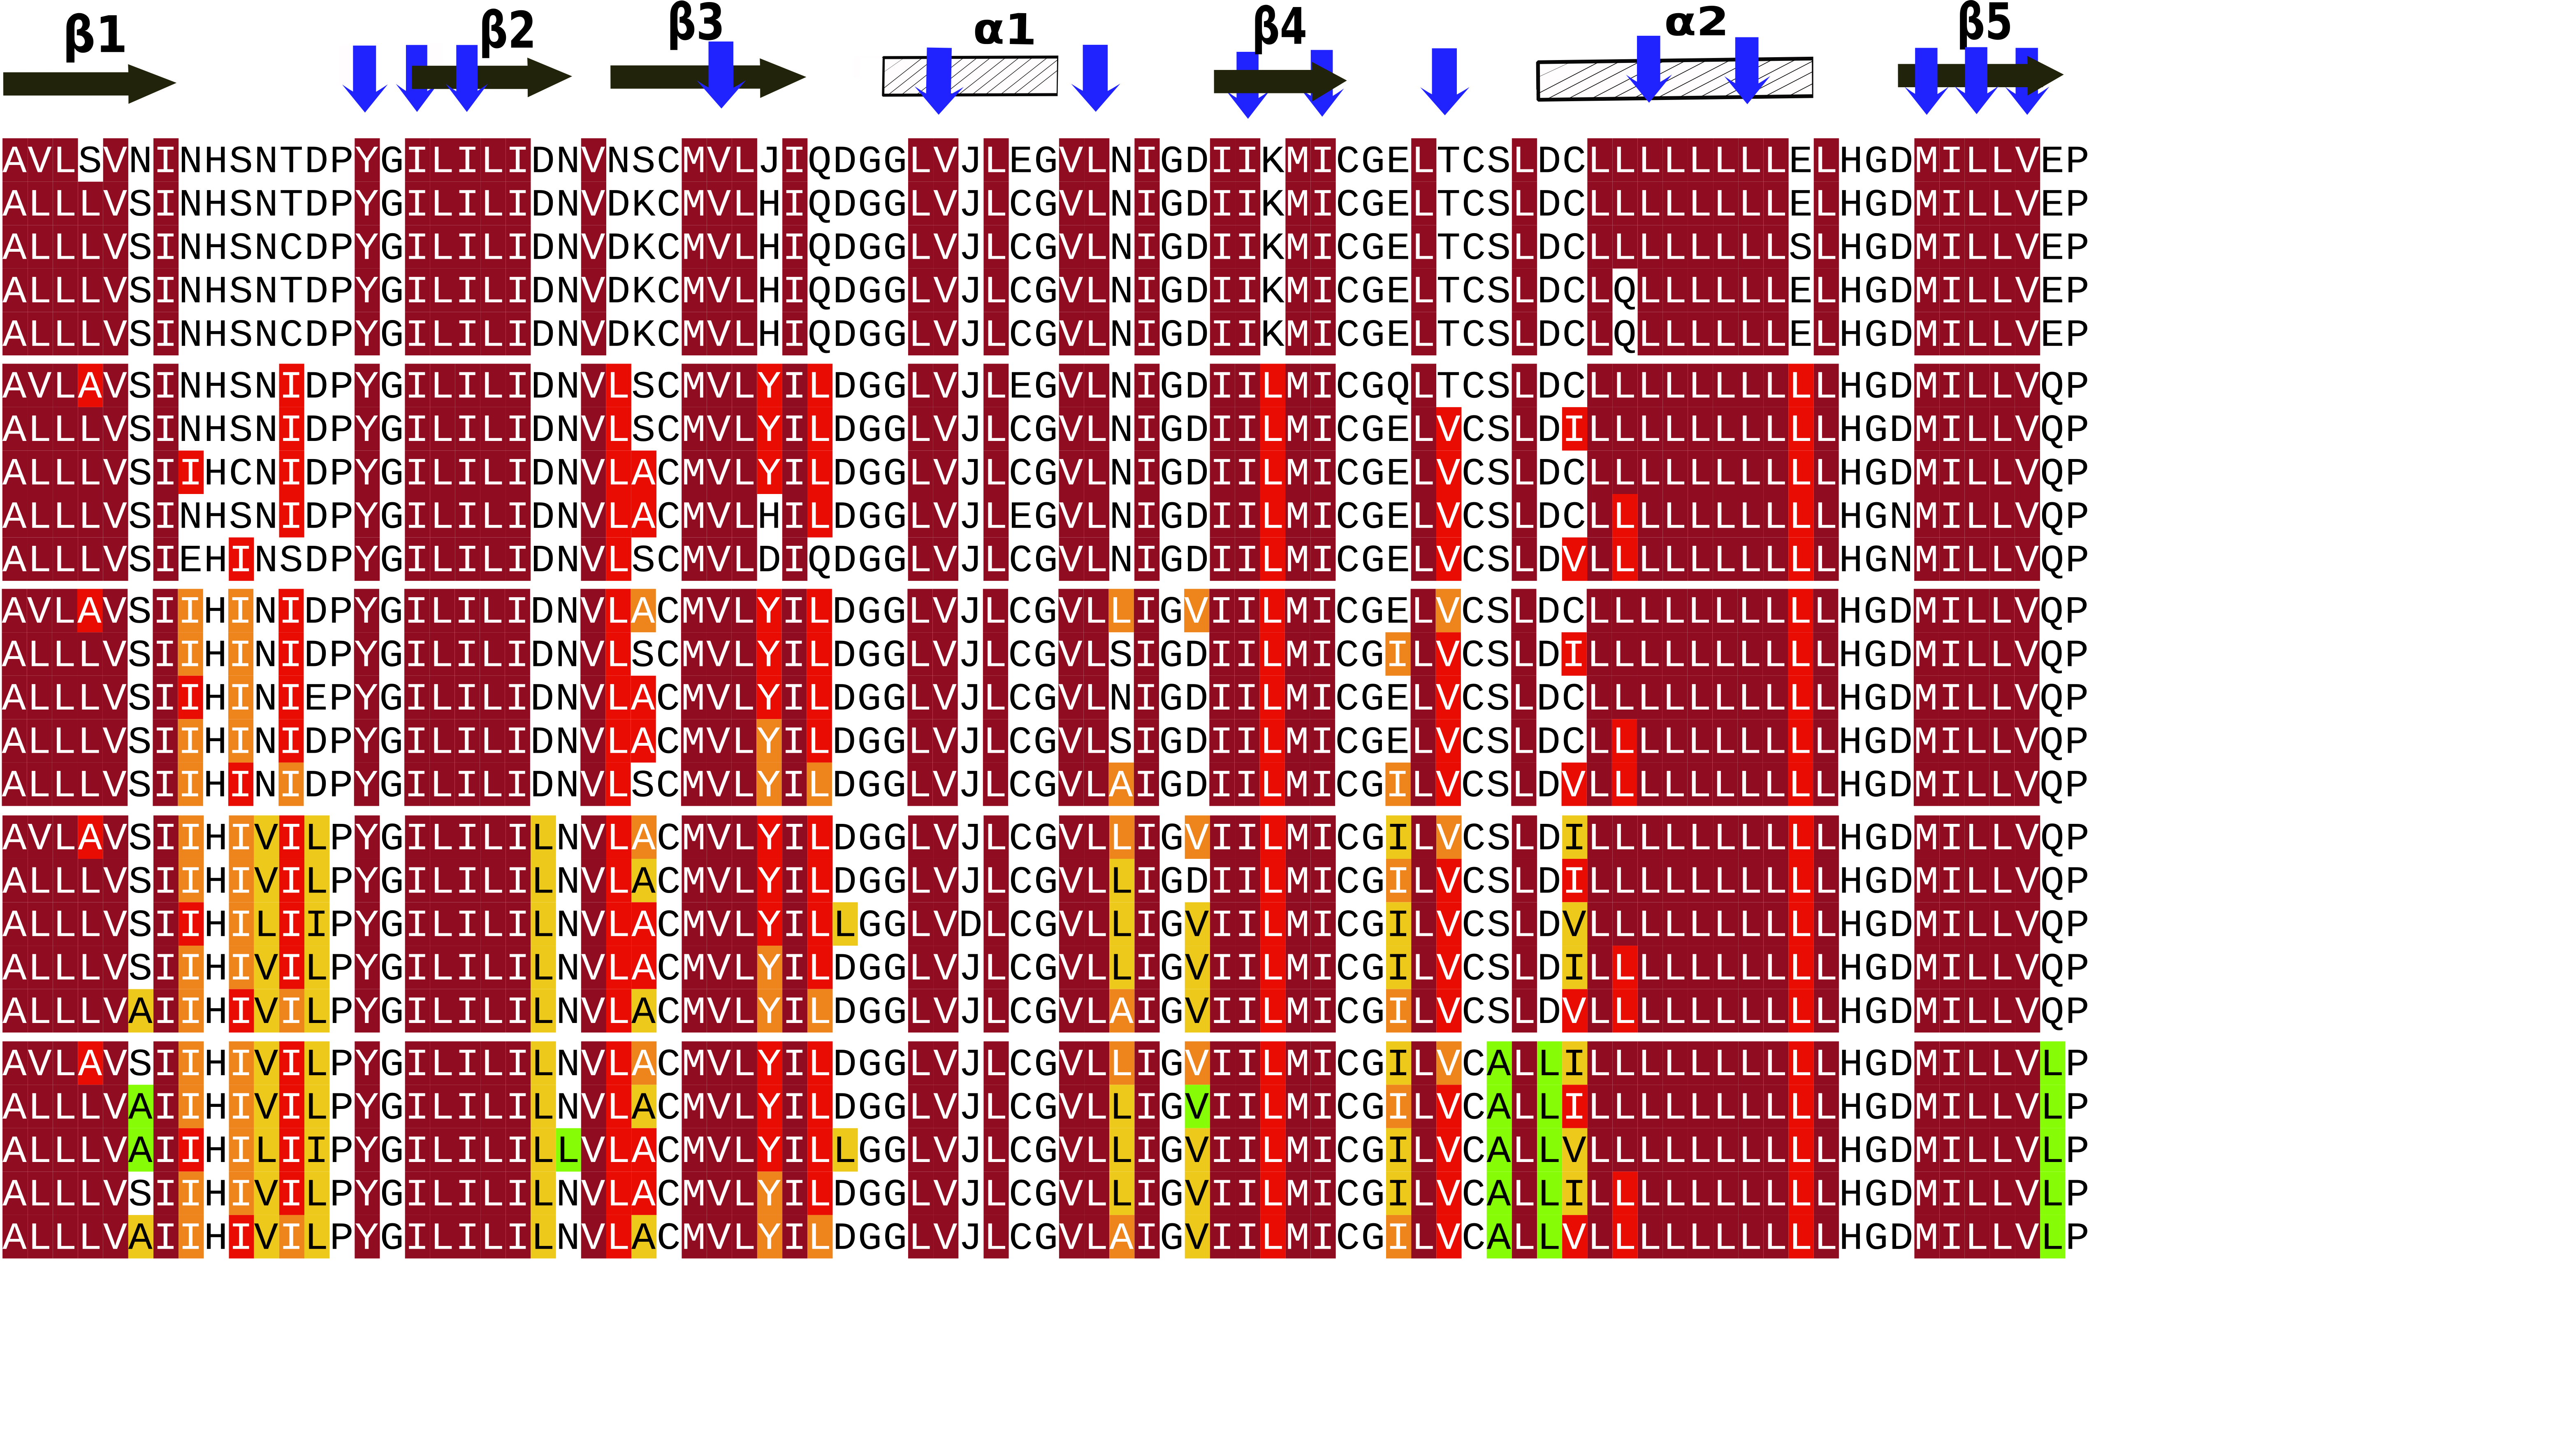
\includegraphics[width=20cm]{boost_hydro/modelA/alignCASK_V2.png} \\
     \end{tabular}
     \caption{Séquences CASK obtenues avec un delta des énergies de références à -0.4,-0.2,0,0.2 et 0.4. Les hydrophobes sont représentés par un dégradé allant du rouge foncé au jaune clair.}
\label{result:PDZ_seed}
   \end{figure}
\end{landscape}

   \clearpage

\begin{landscape}

   \begin{figure}[t]
     \centering
     \begin{tabular}{c}
       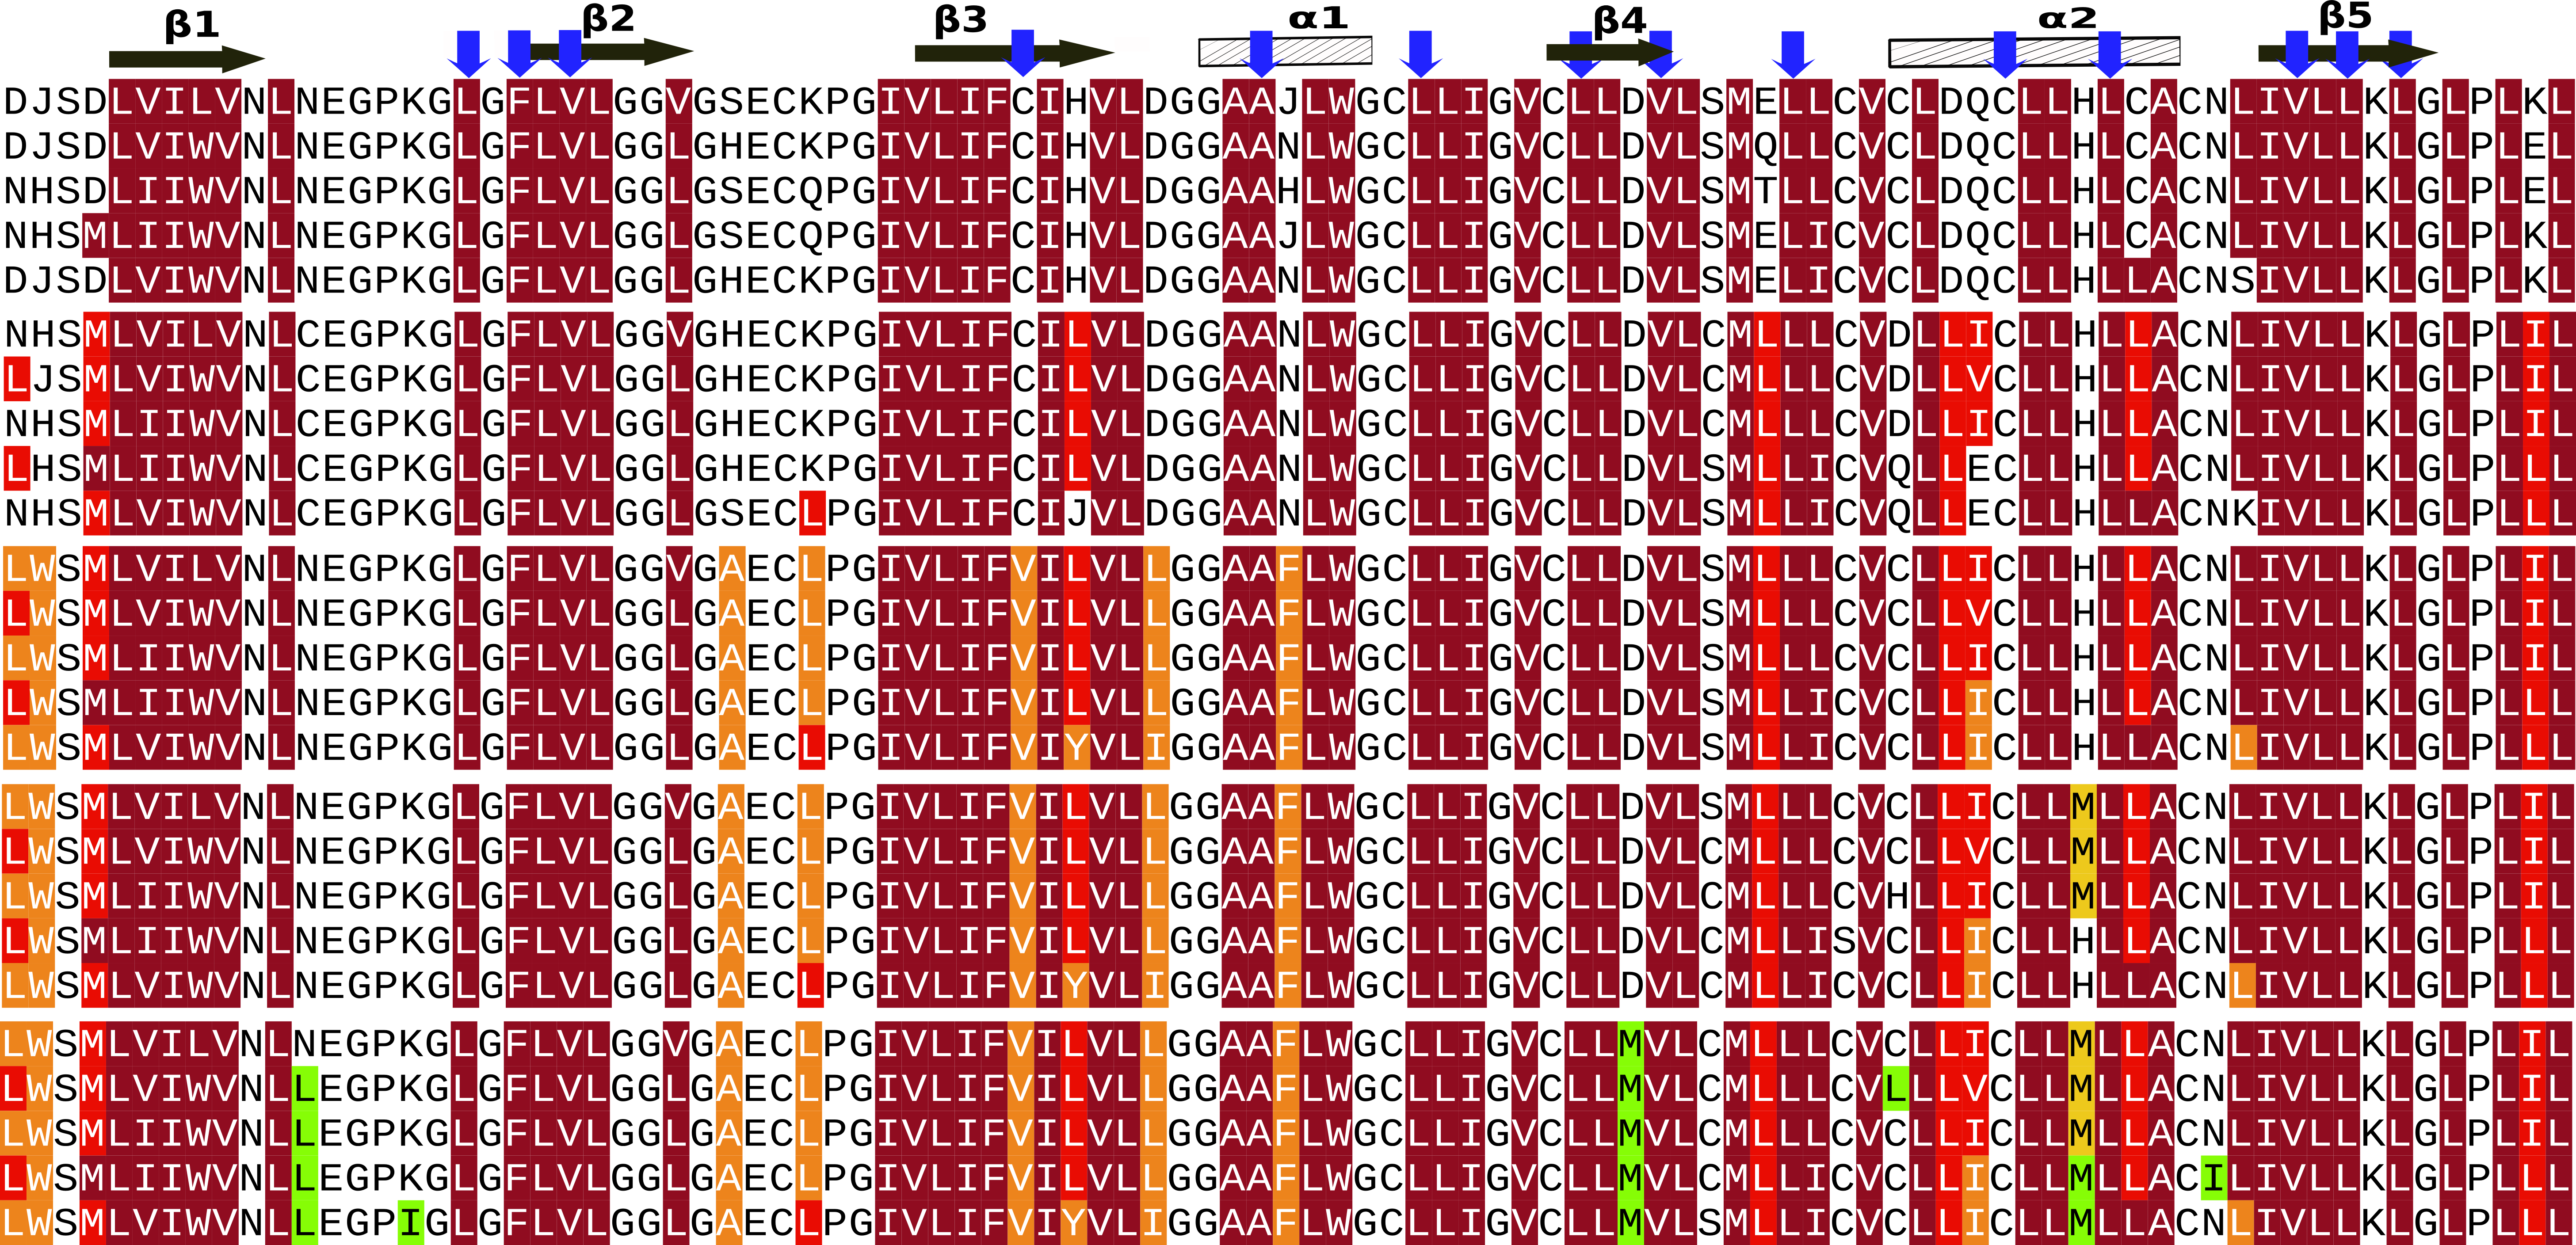
\includegraphics[width=20cm]{boost_hydro/modelA/align2BYG_V2.png} \\
     \end{tabular}
     \caption{Séquences 2BYG obtenues avec un delta des énergies de références à -0.4,-0.2,0,0.2 et 0.4. Les hydrophobes sont représentés par un dégradé allant du rouge foncé au jaune clair.}
\label{result:PDZ_seed}
   \end{figure}
\end{landscape}
   
   \clearpage

   \begin{figure}[t]
     \centering
     \begin{tabular}{c}
       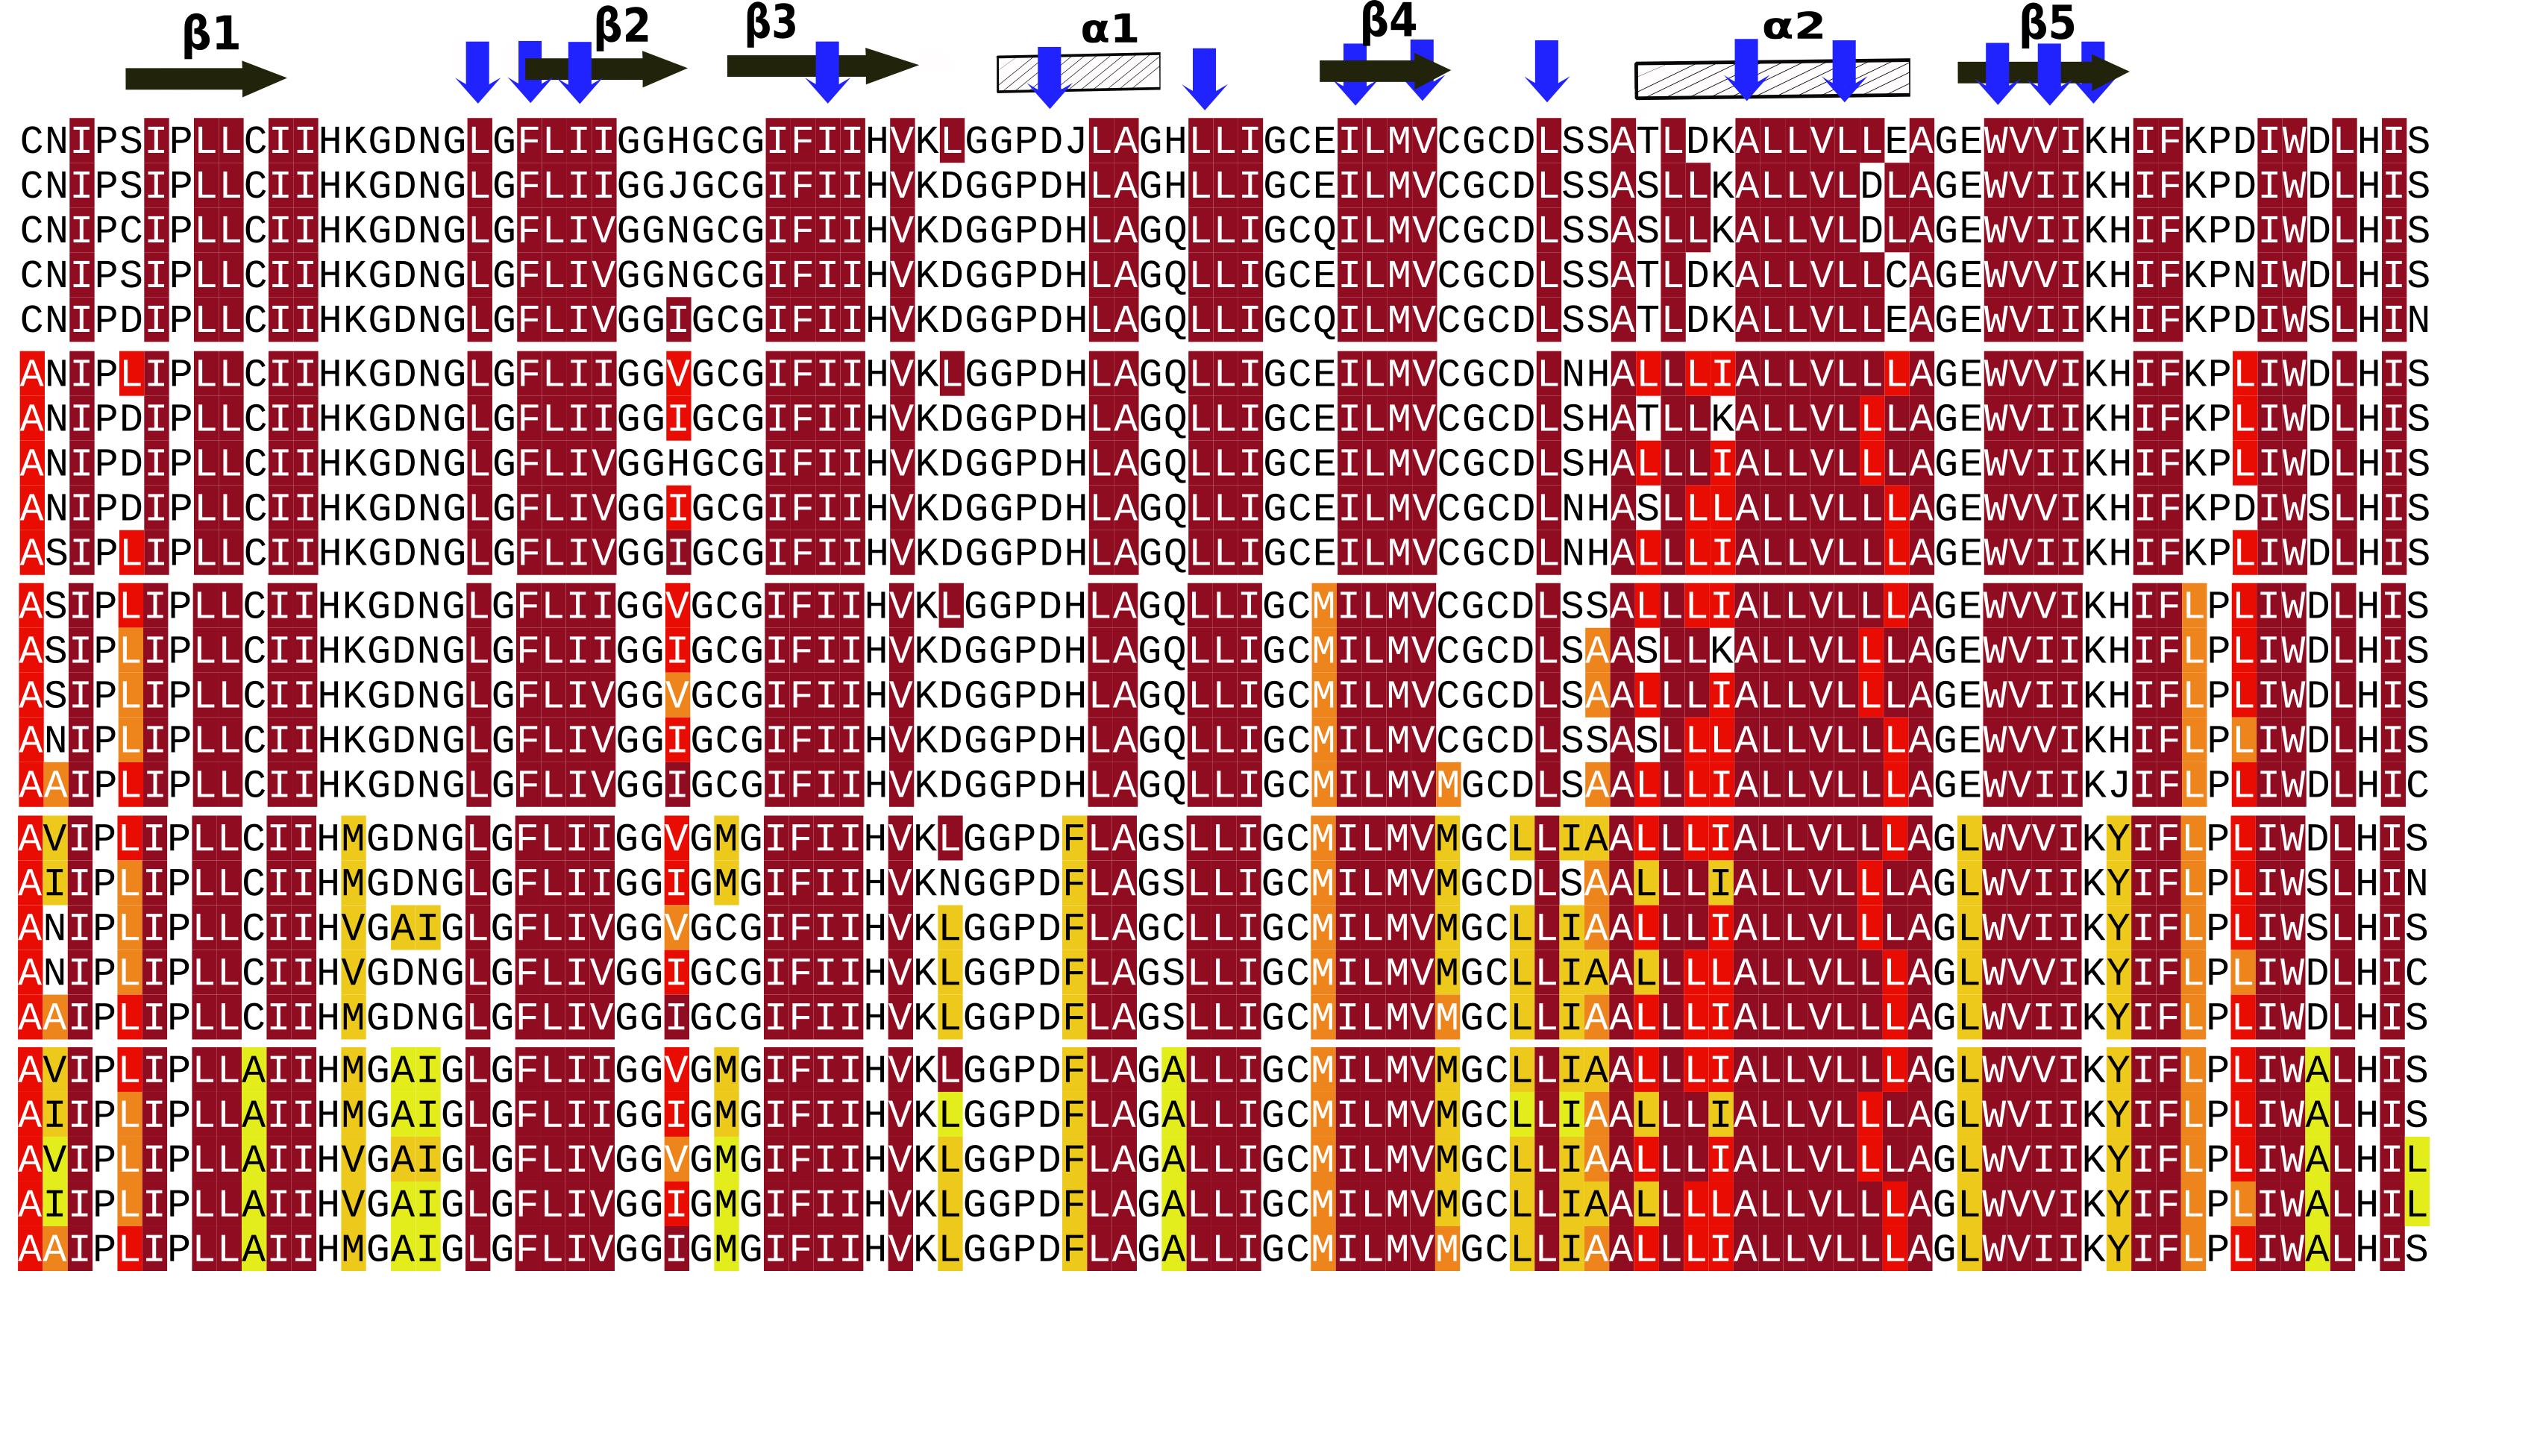
\includegraphics[width=20cm]{boost_hydro/modelA/align3K82.png} \\
     \end{tabular}

     \caption{\small Séquences 3K82 obtenues avec un delta des énergies de références à -0.4,-0.2,0,0.2 et 0.4 .Les hydrophobes pour des deltas de -0.4,-0.2,0,0.2 et 0.4 sont représentés par un dégradé allant du rouge foncé au jaune clair.}

\label{result:PDZ_seed}
   \end{figure}

\end{landscape}


    \clearpage


    \clearpage
    \thispagestyle{empty}
   \begin{figure}[t]
     \centering
     \begin{tabular}{c}
       \includegraphics[width=12cm]{modelB/1R6J_core_simil.png} \\
       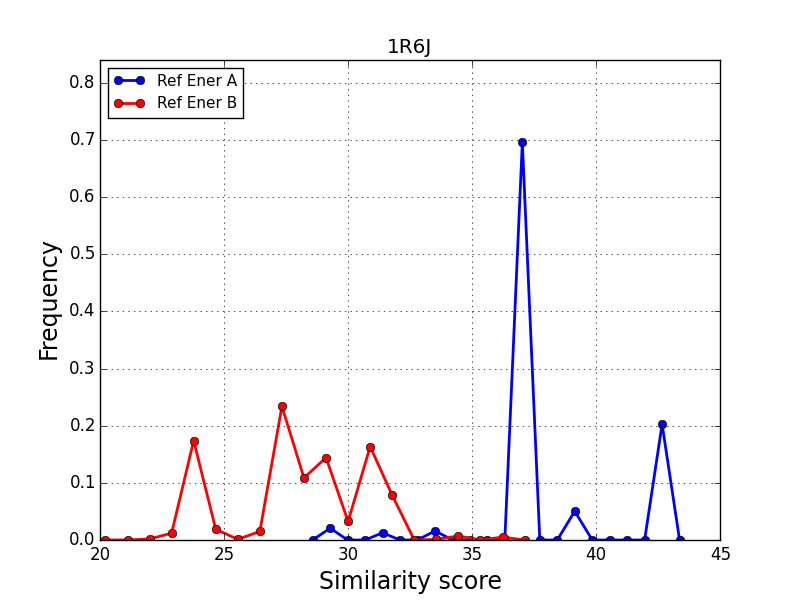
\includegraphics[width=12cm]{modelB/1R6J_simil.png} \\
     \end{tabular}
  \caption{Similarité des séquences 1R6J(modèleB) et Rosetta à l'alignement Pfam RP55,aux positions du cœur (en haut) et sur l'ensemble des positions (en bas).}

\label{graph:Simil_modeB}
   \end{figure}



    \clearpage
    \thispagestyle{empty}
   \begin{figure}[t]
     \centering
     \begin{tabular}{cc}
       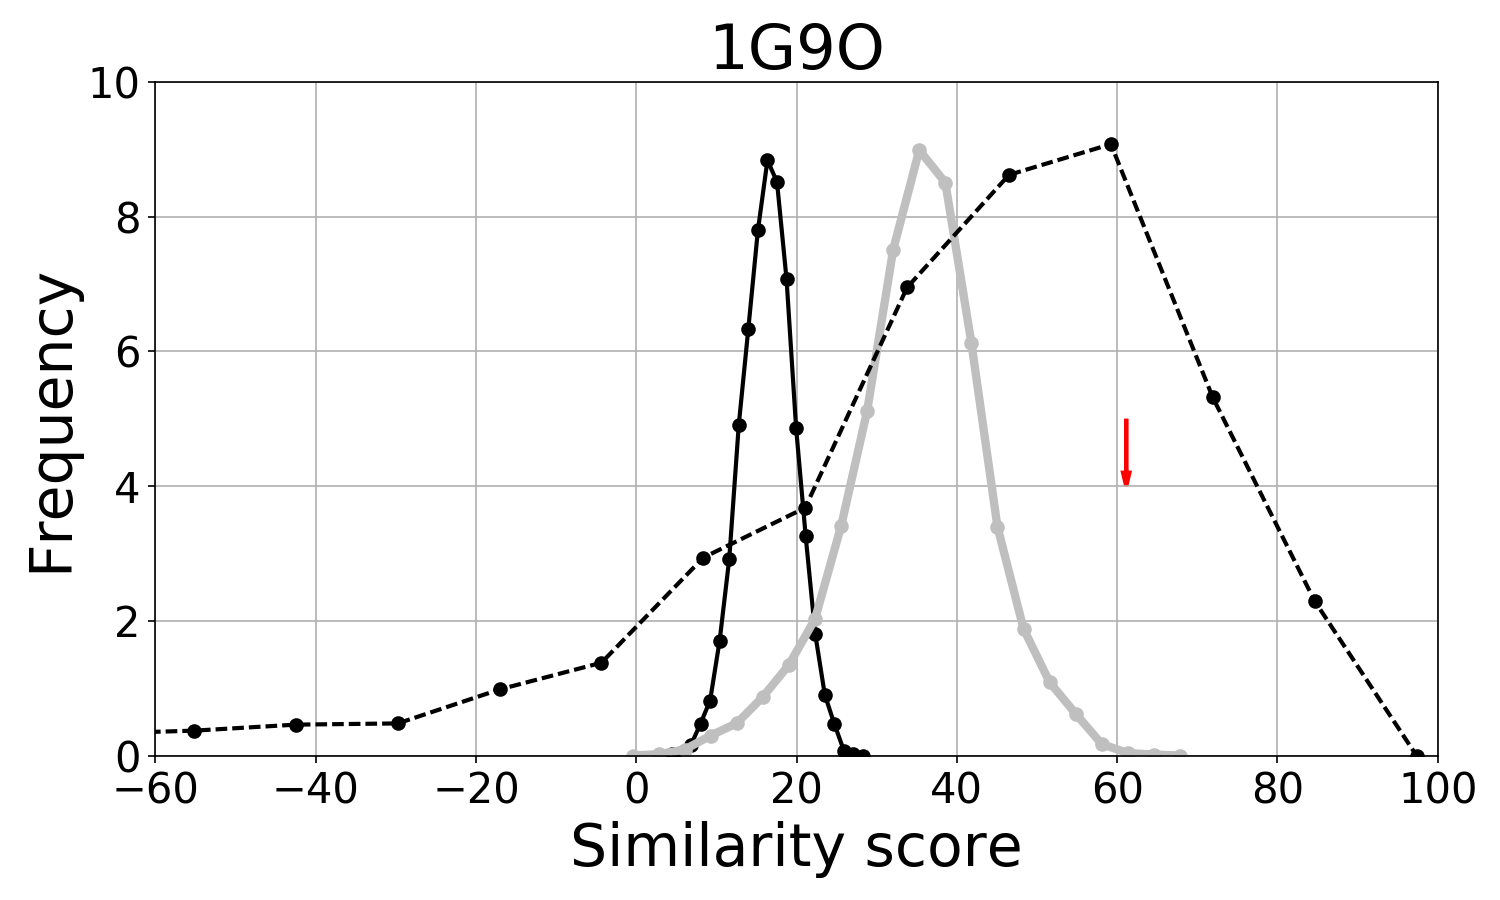
\includegraphics[width=8.4cm]{optGrad0/RP55/1G9O_simil_full.png} &
       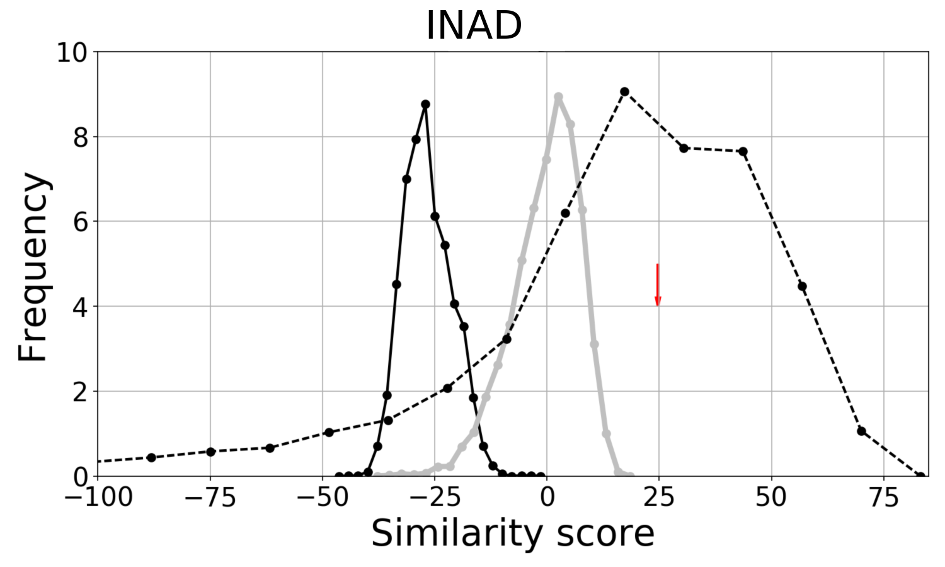
\includegraphics[width=8.4cm]{optGrad0/RP55/1IHJ_simil_full.png} \\
       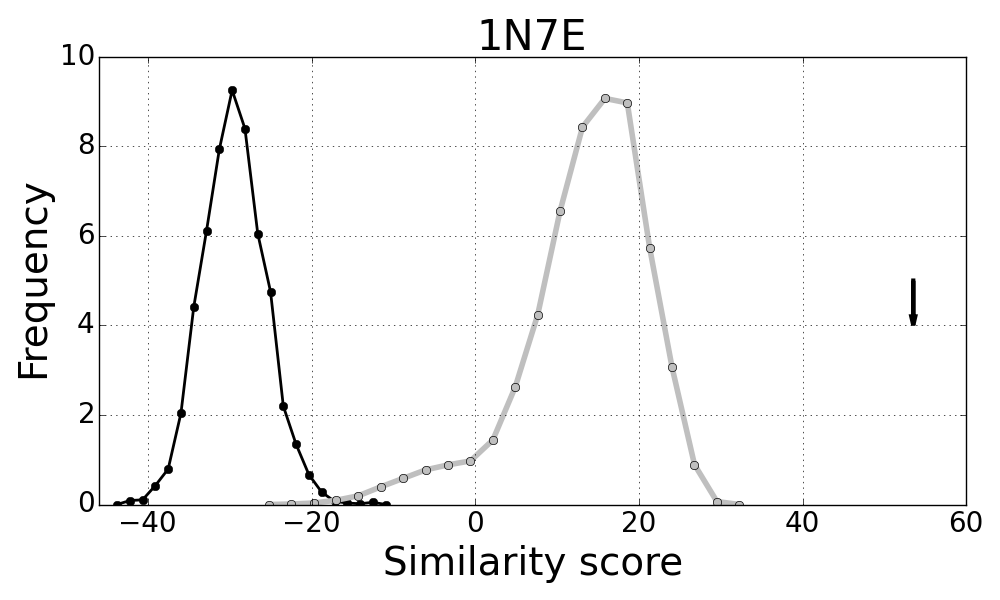
\includegraphics[width=8.4cm]{optGrad0/RP55/1N7E_simil_full.png} &
       \includegraphics[width=8.4cm]{optGrad0/RP55/2BYG_simil_full.png} \\
       \includegraphics[width=8.4cm]{optGrad0/RP55/1R6J_simil_full.png} &
       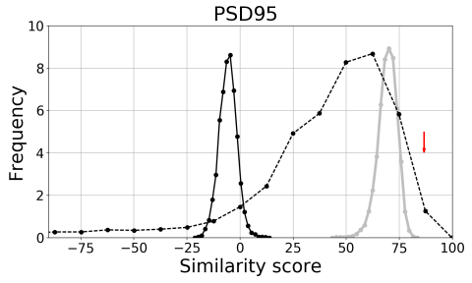
\includegraphics[width=8.4cm]{optGrad0/RP55/3K82_simil_full.png} \\
     \end{tabular}
       \caption{Similarité des séquences Proteus(modèle A) et Rosetta à l'alignement Pfam RP55 sur l'ensemble des positions.}

\label{graph:Simil_Proteus_PDZ_All}
   \end{figure}
   

    \clearpage
    \thispagestyle{empty}
   \begin{figure}[t]
     \centering
     \begin{tabular}{cc} 
       \includegraphics[width=8.4cm]{modelB/1R6J_simil_full.png} &
       \includegraphics[width=8.4cm]{modelB/2BYG_simil_full.png} \\
       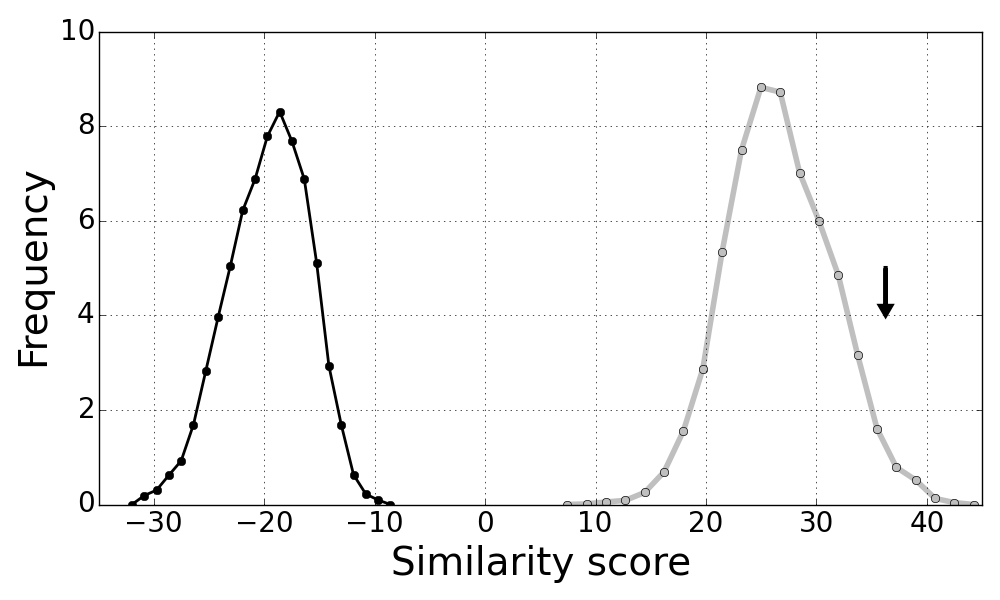
\includegraphics[width=8.4cm]{modelB/1R6J_simil_struct.png} &
       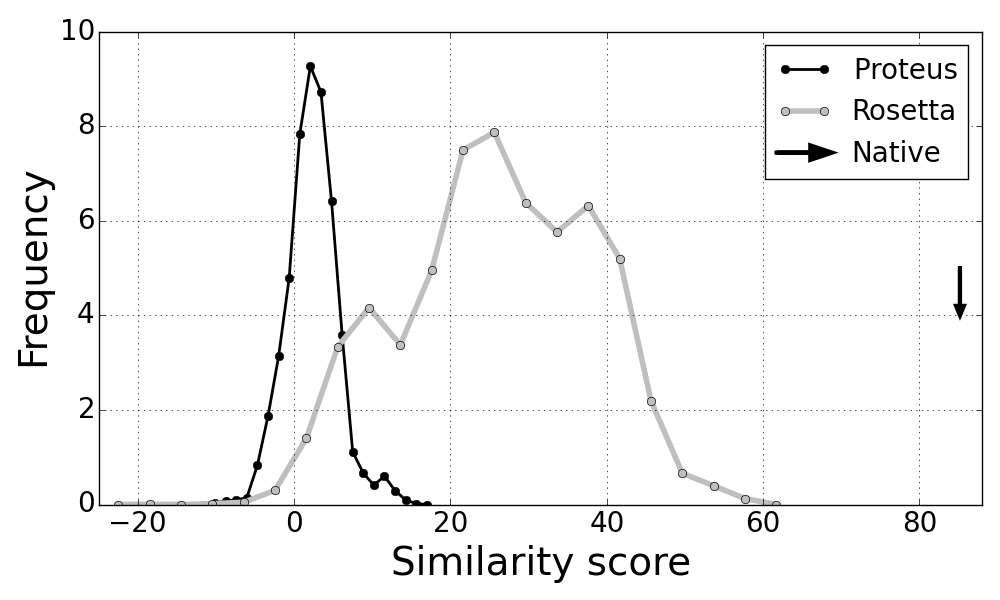
\includegraphics[width=8.4cm]{modelB/2BYG_simil_struct.png} \\
       \includegraphics[width=8.4cm]{modelB/1R6J_simil_core.png} &
       \includegraphics[width=8.4cm]{modelB/2BYG_simil_core.png} \\

     \end{tabular}
  \caption{Similarité des séquences 1R6J et 2BYG produites par proteus modèle B et Rosetta à l'alignement Pfam RP55, sur l'ensemble des positions (au haut),aux positions structurées (au milieu) et sur les positions du coeur (en bas).}

\label{graph:Simil_modeB}
   \end{figure}

    \clearpage
    \thispagestyle{empty}
   \begin{figure}[t]
     \centering
     \begin{tabular}{cc} 
       \includegraphics[width=8.4cm]{modelB/1G9O_simil_full.png} &
       \includegraphics[width=8.4cm]{modelB/1N7E_simil_full.png} \\
       \includegraphics[width=8.4cm]{modelB/1G9O_simil_core.png} &
       \includegraphics[width=8.4cm]{modelB/1N7E_simil_core.png} \\

     \end{tabular}
  \caption{Similarité des séquences 1G9O,1N7E et 3K82 produites par proteus modèle B et Rosetta à l'alignement Pfam RP55, sur l'ensemble des positions (au haut) et sur les positions du coeur (en bas).}

\label{graph:Simil_modeB}
   \end{figure}

   \clearpage   


   
\begin{table}[h]
  \raggedleft{}
  
  \begin{tabular}{cccccc}
    
    \toprule
    Protein & Match/seq & Superfamily & Superfamily & Family & Family \\
            & size      & Evalue      & success     & Evalue & success\\
    \cmidrule{1-6}
    1G9O  & 81/91 & 3.3e-13  & 6656  &  4.0e-3 & 6656 \\
    1IHJ  &  /94 &      &    &   &    \\
    1N7E  & 74/95 & 1.1e-7  & 3754  &  6.9e-3 & 3754 \\
    1R6J  & 67/91 & 6.3e-3  & 6664  &  4.0e-3 & 6664 \\
    2BYG  & 85/97 & 6.0e-9  & 4758  & 5.0e-3  & 4758 \\
    3K82  & /97 &           &   0    &        &  0   \\

    \bottomrule        
  \end{tabular}   
  \caption{Résultats Superfamily pour les séquences Proteus avec le modèle B. --> pas interessant}   
  \label{tab:superfamily}       
\end{table}


   \clearpage   


   
\begin{table}[h]
  \raggedleft{}
  
  \begin{tabular}{cccccc}
    
    \toprule
    Protein & Match/seq & Superfamily & Superfamily & Family & Family \\
            & size      & Evalue      & success     & Evalue & success\\
    \cmidrule{1-6}
    1G9O  & 82/91 & 6.47e-14 & 1000  & 4.70e-3  & 1000 \\
    1IHJ  & 86/94 & 5.93e-11 & 1000  & 2.35e-3  & 1000 \\
    1N7E  & 79/95 & 2.25e-6  & 1000  & 1.16e-2  & 1000 \\
    1R6J  & 62/91 & 9.51e-3  & 9986  & 7.14e-3  & 9986 \\
    2BYG  & 85/97 & 2.98e-9  & 1000  & 4.41e-3  & 1000 \\
    3K82  & 0/97 & 0         &   & 0  &  \\

    \bottomrule        
  \end{tabular}   
  \caption{Résultats Superfamily pour les séquences Proteus avec le modèle B N=6 (convergé au sens des groupes d'aa).}   
  \label{tab:superfamily_model_B6}       
\end{table}


    \clearpage
    \thispagestyle{empty}
   \begin{figure}[t]
     \centering
     \begin{tabular}{cc} 
       \includegraphics[width=8.4cm]{modelB6/1G9O_simil_full.png} &
       \includegraphics[width=8.4cm]{modelB6/1IHJ_simil_full.png} \\
       \includegraphics[width=8.4cm]{modelB6/1R6J_simil_full.png} &
       \includegraphics[width=8.4cm]{modelB6/1N7E_simil_full.png} \\
       \includegraphics[width=8.4cm]{modelB6/2BYG_simil_full.png} &
       \includegraphics[width=8.4cm]{modelB6/3K82_simil_full.png} \\
     \end{tabular}
  \caption{Similarité des séquences des 6 protéines produites par proteus modèle B N=6 (convergé au sens des groupes d'aa) et Rosetta à l'alignement Pfam RP55, sur l'ensemble des positions.}

\label{graph:Simil_modeB}


   \end{figure}



   \begin{table}
     \centering
\caption{La composition en acide aminé (\%) des séquences expérimentales et Proteus après optimisation des énergies de référence. La différence entre expérimentales et Proteus sur les classes est donnée entre crochets.}
\begin{tabular}{l|cccc|cccc}
\hline
\multirow{2}{*}{Res} & \multicolumn{4}{c|}{Experimental n=6}& \multicolumn{4}{c}{Modèle B n=6}\\
 & \multicolumn{2}{c}{Buried} & \multicolumn{2}{c|}{Exposed} & \multicolumn{2}{c}{Buried} & \multicolumn{2}{c}{Exposed} \\
\hline
 & type & classe & type & classe & type & classe & type & classe \\
\hline 
ALA                  & 11.0                 &  \multirow{3}{*}{17.0} & 4.6                  & \multirow{3}{*}{13.4}   &   10.5               & \multirow{2}{*}{11.3}   & 4.4 & \multirow{2}{*}{12.1} \\
CYS                  & 1.3                  &                        & 0.5                  &                         &    0.6               & \multirow{2}{*}{[5.7]}  & 2.3 & \multirow{2}{*}{[1.3]} \\
THR                  & 4.8                  &                        & 8.3                  &                         &    0.2               &                         & 5.4 &                       \\
\hline
\multirow{2}{*}{SER} & \multirow{2}{*}{5.3} & \multirow{2}{*}{5.3}   & \multirow{2}{*}{7.7} & \multirow{2}{*}{7.7}    & \multirow{2}{*}{5.0} &  5.0                    & \multirow{2}{*}{8.1} & 8.1 \\
                     &                      &                        &                      &                         &                      &  [0.3]                  &                      & [-0.4] \\
\hline
ASP                  & 4.3                  & \multirow{2}{*}{6.9}   & 6.0                  & \multirow{2}{*}{17.9}   &   4.4                &  8.5                    & 6.3    & 17.3   \\
GLU                  & 2.6                  &                        & 11.9                 &                         &   4.1                &  [1.4]                  & 11.0   &  [0.6] \\
\hline
ASN                  & 2.6                  & \multirow{2}{*}{4.7}   & 6.7                  & \multirow{2}{*}{12.2}   &   2.0                &  5.6                    & 7.5 & 13.7 \\
GLN                  & 2.1                  &                        & 5.5                  &                         &   3.6                &  [-0.9]                 & 6.2 & [-1.5]    \\
\hline
HIP                  & 1.2                  & \multirow{3}{*}{1.2}   & 5.1                  & \multirow{3}{*}{5.1}    &   1.6                & \multirow{2}{*}{2.2}    & 6.5 & \multirow{2}{*}{8.1} \\
HIE                  & 0.0                  &                        & 0.0                  &                         &   0.3                & \multirow{2}{*}{[-1.0]} & 0.9 & \multirow{2}{*}{[3.0]}  \\
HID                  & 0.0                  &                        & 0.0                  &                         &   0.2                &                         & 0.7 & \\
\hline
ILE                  & 16.0                 & \multirow{3}{*}{50.8}  & 4.2                  & \multirow{3}{*}{14.0}   &   19.3               & \multirow{2}{*}{56.7}   & 5.2 & \multirow{2}{*}{12.4} \\
VAL                  & 16.6                 &                        & 5.4                  &                         &   16.6               & \multirow{2}{*}{[5.9]}  & 4.0 & \multirow{2}{*}{1.6}  \\
LEU                  & 18.2                 &                        & 4.4                  &                         &   20.8               &                         & 3.2 & \\
\hline
\multirow{2}{*}{MET} & \multirow{2}{*}{0.9} & \multirow{2}{*}{0.9}   & \multirow{2}{*}{1.5} & \multirow{2}{*}{1.5}    & \multirow{2}{*}{0.6} & 0.6                    & \multirow{2}{*}{2.3} & 2.3 \\
                     &                      &                        &                      &                         &                      & [0.3]                  &                      & [-0.8] \\
\hline
\multirow{2}{*}{LYS} & \multirow{2}{*}{2.5} & \multirow{2}{*}{2.5}   & \multirow{2}{*}{10.9} & \multirow{2}{*}{10.9}  & \multirow{2}{*}{1.5} &   1.5                   & \multirow{2}{*}{12.9} & 12.9 \\
                     &                      &                        &                       &                        &                      &  [1.0]                  &                       & [2.0] \\
\hline
\multirow{2}{*}{ARG} & \multirow{2}{*}{2.9} & \multirow{2}{*}{2.9}   & \multirow{2}{*}{8.8} & \multirow{2}{*}{8.8}    & \multirow{2}{*}{1.4} & 1.4                    & \multirow{2}{*}{11.4}  & 11.4 \\
                     &                      &                         &                      &                        &                      & [1.5]                  &                        & [-2.6]   \\
\hline
PHE                  & 4.2                  & \multirow{2}{*}{4.2}   & 2.4                  & \multirow{2}{*}{2.4}    &  3.9                 & 4.8                    & 0.4 & 0.7 \\
THP                  & 0.0                  &                        & 0.0                  &                         &  0.9                 & [-0.6]                 & 0.3 & [1.7]               \\
\hline
\multirow{2}{*}{TYR} & \multirow{2}{*}{2.5} & \multirow{2}{*}{2.5}   & \multirow{2}{*}{1.2} & \multirow{2}{*}{1.2}   & \multirow{2}{*}{2.3}  & 2.3                     & \multirow{2}{*}{0.1} & 0.1\\
                     &                      &                        &                      &                         &                      &  [0.2]                  &                      & [1.1]   \\
\hline
GLY                  & 0.1                  & \multirow{2}{*}{0.1}   & 3.1                  & \multirow{2}{*}{4.9}    &   0.0                &  0.0                    & 0.0 & 0.0 \\
PRO                  & 0.0                  &                        & 1.8                  &                         &   0.0                &  [0.1]                  & 0.0 & [4.9]\\
\hline

\end{tabular} 
\end{table}

   \clearpage
\begin{table}[h]
  \raggedleft{}
  
  \begin{tabular}{cccccc}
    
    \toprule
    Protein & Match/seq & Superfamily & Superfamily & Family & Family \\
            & size      & Evalue      & success     & Evalue & success\\
    \cmidrule{1-6}
    1G9O  & 81/91 &  2.00e-12 & 10000  & 9.97e-3 & 10000  \\
    1IHJ  & 84/94 &  4.80e-11 & 10000  & 2.83e-3 & 10000  \\
    1N7E  & 82/95 &  4.73e-8  & 10000  & 5.56e-3 & 10000  \\
    1R6J  & 63/91 &  4.01e-4  &  9999  & 1.05e-2 &  9999  \\
    2BYG  & 84/97 &  3.82e-10 & 10000  & 3.75e-3 & 10000  \\
    3K82  & 46/97 &  7.65e-1  &  5029  & 4.06e-2 &  4719  \\

    \bottomrule        
  \end{tabular}   
  \caption{Résultats Superfamily pour les séquences Proteus avec le modèle B N=6 (E ref optimisées sur 20 cycles selon les classes + 20 cycles selon les types).}   
  \label{tab:superfamily_model_B6}       
\end{table}
   

    \clearpage
    \thispagestyle{empty}
   \begin{figure}[t]
     \centering
     \begin{tabular}{cc} 
       \includegraphics[width=8.4cm]{modelB6+/1G9O_simil_full.png} &
       \includegraphics[width=8.4cm]{modelB6+/1IHJ_simil_full.png} \\
       \includegraphics[width=8.4cm]{modelB6+/1R6J_simil_full.png} &
       \includegraphics[width=8.4cm]{modelB6+/1N7E_simil_full.png} \\
       \includegraphics[width=8.4cm]{modelB6+/2BYG_simil_full.png} &
       \includegraphics[width=8.4cm]{modelB6+/3K82_simil_full.png} \\
     \end{tabular}
  \caption{Similarité des séquences des 6 protéines produites par proteus modèle B N=6 (E ref optimisées sur 20 cycles selon les classes + 20 cycles selon les types) et Rosetta à l'alignement Pfam RP55, sur l'ensemble des positions.}

\label{graph:Simil_modeB6+_core}


   \end{figure}


    \clearpage
    \thispagestyle{empty}
   \begin{figure}[t]
     \centering
     \begin{tabular}{cc} 
       \includegraphics[width=8.4cm]{modelB6+/1G9O_simil_core.png} &
       \includegraphics[width=8.4cm]{modelB6+/1IHJ_simil_core.png} \\
       \includegraphics[width=8.4cm]{modelB6+/1R6J_simil_core.png} &
       \includegraphics[width=8.4cm]{modelB6+/1N7E_simil_core.png} \\
       \includegraphics[width=8.4cm]{modelB6+/2BYG_simil_core.png} &
       \includegraphics[width=8.4cm]{modelB6+/3K82_simil_core.png} \\
     \end{tabular}
  \caption{Similarité des séquences des 6 protéines produites par proteus modèle B N=6 (E ref optimisées sur 20 cycles selon les classes + 20 cycles selon les types) et Rosetta à l'alignement Pfam RP55, sur les positions du coeur.}

\label{graph:Simil_modeB6+_core}


   \end{figure}




    \clearpage
    \thispagestyle{empty}
   \begin{figure}[t]
     \centering
     \begin{tabular}{c} 
       \includegraphics[width=15cm]{modelB6+/3K82_seqlogo.eps} \\

     \end{tabular}
  \caption{Séquences 3K82 modèle B N=6,sur les positions du coeur.}

\label{graph:seqlogo_3K82_core}


   \end{figure}

    \clearpage
    \thispagestyle{empty}
   \begin{figure}[t]
     \centering
     \begin{tabular}{cc} 
       \includegraphics[width=8.4cm]{modelB/1R6J_simil_core.png} &
       \includegraphics[width=8.4cm]{modelB/2BYG_simil_core.png} \\
       \includegraphics[width=8.4cm]{modelB/1R6J_simil_cut.png} &
       \includegraphics[width=8.4cm]{modelB/2BYG_simil_cut.png} \\
     \end{tabular}
  \caption{Similarité des séquences produites par proteus modèle B N=2 et Rosetta à l'alignement Pfam RP55, sur les positions du coeur en haut et sur toutes les positions en bas.}

\label{graph:Simil_modeB2core+cut}


   \end{figure}

   


    \clearpage
    \thispagestyle{empty}
   \begin{figure}[t]
     \centering
     \begin{tabular}{cc} 
       \includegraphics[width=8.4cm]{modelB6+/1R6J_simil_core.png} &
       \includegraphics[width=8.4cm]{modelB6+/2BYG_simil_core.png} \\
       \includegraphics[width=8.4cm]{modelB6+/1R6J_simil_cut.png} &
       \includegraphics[width=8.4cm]{modelB6+/2BYG_simil_cut.png} \\
     \end{tabular}
  \caption{Similarité des séquences produites par proteus modèle B N=6 et Rosetta à l'alignement Pfam RP55, sur les positions du coeur en haut et sur toutes les positions en bas.}

\label{graph:Simil_modeB6core+cut}


   \end{figure}


   

   \clearpage

\begin{landscape}

   \begin{figure}[t]
     \centering
     \begin{tabular}{c}
       \includegraphics[width=20cm]{boost_hydro/modelB2/alignCASK.pdf} \\
     \end{tabular}
     \caption{Séquences CASK modèle B N=2 obtenues avec un delta des énergies de références à -0.4,-0.2,0,0.2 et 0.4. Les hydrophobes sont représentés par un dégradé allant du rouge foncé au jaune clair.}
\label{result:titra_CASK_modelB2}
   \end{figure}
\end{landscape}
   

   \clearpage

\begin{landscape}

   \begin{figure}[t]
     \centering
     \begin{tabular}{c}
       \includegraphics[width=20cm]{boost_hydro/modelB2/alignTiam1.pdf} \\
     \end{tabular}
     \caption{Séquences Tiam1 modèle B N=2 obtenues avec un delta des énergies de références à -0.4,-0.2,0,0.2 et 0.4. Les hydrophobes sont représentés par un dégradé allant du rouge foncé au jaune clair.}
\label{result:titra_Tiam1_modelB2}
   \end{figure}
\end{landscape}


    \clearpage
    \thispagestyle{empty}
   \begin{figure}[t]
     \centering
     \begin{tabular}{cc} 
       \includegraphics[width=8.4cm]{modelExactGB/1G9O_simil_cut.png} &
       \includegraphics[width=8.4cm]{modelExactGB/1G9O_simil_core.png} \\
       \includegraphics[width=8.4cm]{modelExactGB/1R6J_simil_cut.png} &
       \includegraphics[width=8.4cm]{modelExactGB/1R6J_simil_core.png} \\
       \includegraphics[width=8.4cm]{modelExactGB/2BYG_simil_cut.png} &
       \includegraphics[width=8.4cm]{modelExactGB/2BYG_simil_core.png} \\
     \end{tabular}
  \caption{Similarité des séquences produites par proteus modèle exactGB  (E ref optimisées selon les classes puis selon les types) et Rosetta à l'alignement Pfam RP55, sur toutes les postions à gauche  et sur les positions du coeur à droite.}

\label{graph:Simil_modelExactGB}


   \end{figure}


   \clearpage
\begin{table}[h]
  \raggedleft{}
  
  \begin{tabular}{cccccc}
    
    \toprule
    Protein & Match/seq & Superfamily & Superfamily & Family & Family \\
            & size      & Evalue      & success     & Evalue & success\\
    \cmidrule{1-6}
    1G9O  & 80/91 &  8.54e-14  & 10000  & 8.94e-3 & 10000  \\
    1R6J  & 70/82 &  2.85e-6   & 10000  & 2.69e-3 & 10000  \\
    2BYG  & 88/97 &  3.26e-12  & 10000  & 1.96e-3 & 10000  \\

    \bottomrule        
  \end{tabular}   
  \caption{Résultats Superfamily pour les séquences Proteus avec le modèle exactGB (E ref optimisées sur 20 cycles selon les classes + 20 cycles selon les types).}   
  \label{tab:superfamily_model_B6}       
\end{table}

\begin{table}[h]
  \begin{tabular}{cccccc}
    
    \toprule
    Protein & Match/seq & Superfamily & Superfamily & Family & Family \\
            & size      & Evalue      & success     & Evalue & success\\
    \cmidrule{1-6}
    1G9O  & 79/91   &    1.3e-13 & 10000 & 2.2e-3 & 10000 \\
    1R6J  & 76/82   &    7.3e-13 & 10000 & 1.8e-3 & 10000 \\
    2BYG  & 86/97   &    1.3e-9  & 10000 & 9.6e-4 & 10000 \\

    \bottomrule        
  \end{tabular}   
  \caption{Résultats Superfamily pour les séquences Rosetta }   
  \label{tab:superfamily_model_B6}       
\end{table}

\begin{table}[h]
  \raggedleft{}
  
  \begin{tabular}{cccccc}
    
    \toprule
    Protein & Match/seq & Superfamily & Superfamily & Family & Family \\
            & size      & Evalue      & success     & Evalue & success\\
    \cmidrule{1-6}
    1G9O  & 62/91 & 3.22 10^{-3}  & 9857  & 1.00 10^{-2} & 9857 \\
    1R6J  & 70/82 & 2.83 10^{-3}  & 9879  & 3.62 10^{-3} & 9879 \\
    2BYG  & 83/97 & 1.66 10^{-3}  & 9876  & 3.18 10^{-3} & 9876 \\

    \bottomrule        
  \end{tabular}   
  \caption{Résultats Superfamily pour les séquences Proteus avec le modèle GB NEA $\epsilon$=4 (E ref optimisées sur 20 cycles selon les classes + 20 cycles selon les types).}   
  \label{tab:superfamily_model_B6}       
\end{table}


   \clearpage
\begin{table}[h]
  \raggedleft{}

  \begin{tabular}{ccc|cc}
    
    \toprule
               & \multicolumn{2}{c|}{Proteus} & \multicolumn{2}{c}{Rosetta} \\
    \cmidrule{1-5}
    Protein    & Family & Family  & Family & Family \\
               & Evalue & success & Evalue & success \\
    \cmidrule{1-5}
    NHREF         & 8.94 10^{-2} & 10000  & 2.2  10^{-3} & 10000 \\
    Syntenin      & 2.69 10^{-3} & 10000  & 1.8  10^{-3} & 10000 \\
    DLG2          & 1.96 10^{-3} & 10000  & 9.6  10^{-4} & 10000 \\
    Tiam1         & 1.96 10^{-3} & 10000  & 2.8  10^{-2} &  9030 \\
    Cask          & 1.96 10^{-3} & 10000  & 7.5  10^{-3} &  9832 \\

    \bottomrule        
  \end{tabular}   
  \caption{}   
  \label{AMMIB}       
\end{table}


   \clearpage
\begin{table}[h]
  \raggedleft{}
  
  \begin{tabular}{cccccc}
    
    \toprule
    Protein & Match/seq & Superfamily & Superfamily & Family & Family \\
            & size      & Evalue      & success     & Evalue & success\\
    \cmidrule{1-6}
    1G9O  & 62/91 & 3.22 10^{-3}  & 9857  & 1.00 10^{-2} & 9857 \\
    1R6J  & 70/82 & 2.83 10^{-3}  & 9879  & 3.62 10^{-3} & 9879 \\
    2BYG  & 83/97 & 1.66 10^{-3}  & 9876  & 3.18 10^{-3} & 9876 \\

    \bottomrule        
  \end{tabular}   
  \caption{Résultats Superfamily pour les séquences Proteus avec le modèle GB NEA $\epsilon$=4 (E ref optimisées sur 20 cycles selon les classes + 20 cycles selon les types).}   
  \label{tab:superfamily_model_B6}       
\end{table}

    \clearpage
    \thispagestyle{empty}
   \begin{figure}[t]
     \centering
     \begin{tabular}{cc} 
       \includegraphics[width=8.4cm]{neaGB4/1G9O_simil_cut.png} &
       \includegraphics[width=8.4cm]{neaGB4/1G9O_simil_core.png} \\
       \includegraphics[width=8.4cm]{neaGB4/1R6J_simil_cut.png} &
       \includegraphics[width=8.4cm]{neaGB4/1R6J_simil_core.png} \\
       \includegraphics[width=8.4cm]{neaGB4/2BYG_simil_cut.png} &
       \includegraphics[width=8.4cm]{neaGB4/2BYG_simil_core.png} \\
     \end{tabular}
     \caption{Similarité des séquences produites par proteus modèle GB NEA $\epsilon$=4, E ref optimisées selon les classes puis selon les types et Rosetta à l'alignement Pfam RP55, sur toutes les positions à gauche  et sur les positions du coeur à droite.}

\label{graph:Simil_modelExactGB}


   \end{figure}


       \clearpage
    \thispagestyle{empty}
   \begin{figure}[t]
     \centering
     \begin{tabular}{cc} 
       \includegraphics[width=8.4cm]{control/1G9O_simil_cut.png} &
       \includegraphics[width=8.4cm]{control/1G9O_simil_core.png} \\
       \includegraphics[width=8.4cm]{control/1R6J_simil_cut.png} &
       \includegraphics[width=8.4cm]{control/1R6J_simil_core.png} \\
       \includegraphics[width=8.4cm]{control/2BYG_simil_cut.png} &
       \includegraphics[width=8.4cm]{control/2BYG_simil_core.png} \\
     \end{tabular}
     \caption{Similarité des séquences produites Rosetta , et des séquences de l'aligenment Pfam RP55, sur toutes les positions à gauche  et sur les positions du coeur à droite.}

\label{graph:Simil_control}


   \end{figure}



       \clearpage
    \thispagestyle{empty}
   \begin{figure}[t]
     \centering
     \begin{tabular}{cc} 
       \includegraphics[width=8.4cm]{exactGB/1G9O_simil_cut.png} &
       \includegraphics[width=8.4cm]{exactGB/1G9O_simil_core.png} \\
       \includegraphics[width=8.4cm]{exactGB/1R6J_simil_cut.png} &
       \includegraphics[width=8.4cm]{exactGB/1R6J_simil_core.png} \\
       \includegraphics[width=8.4cm]{exactGB/2BYG_simil_cut.png} &
       \includegraphics[width=8.4cm]{exactGB/2BYG_simil_core.png} \\
     \end{tabular}
%     \caption{Similarité des séquences Proteus (NEA et FDB),Rosetta , et des séquences de l'aligenment Pfam RP55, sur toutes les positions à gauche  et sur les positions du coeur à droite.}

\label{graph:Simil_control_B}


   \end{figure}


   \clearpage
   
    \begin{table}[!htbp]
      \centering

      \begin{tabular}{ccc|cc}

        \toprule
        \multirow{2}{*}{acides aminés}  & \multicolumn{2}{c|}{NEA} & \multicolumn{2}{c}{FDB} \\
        \cmidrule{2-5}
         & Pos. Enf. & Pos Exp. & Pos. Enf. & Pos Exp. \\
        \cmidrule{1-5}

        ALA &   0.00     &  0.00    &   0.00  &   0.00       \\
        CYS &  -0.89     &  -2.57   &  -1.06  &   -1.64      \\
        THR &  -5.31     &  -8.075  &  -4.84  &   -6.68      \\
        SER &  -5.55     &  -6.55   &  -4.45  &   -5.24      \\
        ASP &  -17.26    &  -22.06  &  -14.56 &   -18.82     \\
        GLU &  -16.12    &  -20.68  &  -14.52 &   -18.21     \\
        ASN &  -16.38    &  -20.41  &  -14.02 &   -17.80     \\
        GLN &  -14.00    &  -18.41  &  -13.14 &   -16.61     \\
        HID &   11.21    &  6.95    &  10.85  &   8.13       \\
        HIE &   10.63    &  6.15    &  10.41  &   7.37       \\
        HIP &   15.17    &  10.72   &  12.86  &   10.98      \\
        ARG &  -53.40    &  -57.36  &  -51.37 &   -54.76     \\
        LYS &  -8.20     &  -12.34  &  -8.24  &   -11.35     \\
        ILE &   6.76     &  3.44    &  5.50   &   3.06       \\
        VAL &   0.43     &  -2.19   &  -0.05  &   -1.66      \\
        LEU &   0.52     &  -3.72   &  0.00   &   -2.94      \\
        MET &  -1.61     &  -3.21   &  -2.85  &   -3.09      \\
        PHE &   1.86     &  -2.68   &  0.17   &   -3.18      \\
        TRP &  -0.23     &  -7.67   &  -1.94  &   -5.53      \\
        TYR &  -5.10     &  -10.90  &  -5.91  &   -10.14     \\

        \bottomrule


      \end{tabular}      
      \caption{Les énergies de référence obtenues avec l'optimisation 6 protéines.}
\label{tab:RefEner_groupes}      
    \end{table}

    \clearpage

   \begin{table}
     \centering
\caption{La composition en acide aminé (\%) des séquences expérimentales et Proteus après optimisation des énergies de référence. La différence entre expérimentales et Proteus sur les classes est donnée entre crochets.}
\begin{tabular}{l|cccc|cccc}
\hline
\multirow{2}{*}{Res} & \multicolumn{4}{c|}{Experimental n=3}& \multicolumn{4}{c}{FDB}\\
 & \multicolumn{2}{c}{Buried} & \multicolumn{2}{c|}{Exposed} & \multicolumn{2}{c}{Buried} & \multicolumn{2}{c}{Exposed} \\
\hline
 & type & classe & type & classe & type & classe & type & classe \\
\hline 
ALA                  & 8.7                  &  \multirow{3}{*}{16.8} & 5.5                  & \multirow{3}{*}{13.6}   &   9.6                & \multirow{2}{*}{17.1}    & 1.8 & \multirow{2}{*}{11.3} \\
CYS                  & 1.9                  &                        & 0.4                  &                         &    2.8               & \multirow{2}{*}{[-0.3]}  & 0.6 & \multirow{2}{*}{[2.3]} \\
THR                  & 6.2                  &                        & 7.7                  &                         &    4.7               &                          & 8.9 &                       \\
\hline
\multirow{2}{*}{SER} & \multirow{2}{*}{4.4} & \multirow{2}{*}{4.4}   & \multirow{2}{*}{6.7} & \multirow{2}{*}{6.7}    & \multirow{2}{*}{5.2} & 5.2                      & \multirow{2}{*}{7.9} & 7.9\\
                     &                      &                        &                      &                         &                      &  [-0.8]                  &                      & [-1.2] \\
\hline
ASP                  & 4.8                  & \multirow{2}{*}{7.4}   & 6.1                  & \multirow{2}{*}{17.1}   &   5.8                &  8.6                     & 8.1    & 20.6  \\
GLU                  & 2.6                  &                        & 11.0                 &                         &   2.8                &  [-1.2]                  & 12.5   &  [-3.5] \\
\hline
ASN                  & 3.4                  & \multirow{2}{*}{5.1}   & 6.9                  & \multirow{2}{*}{12.7}   &   4.2                &  6.0                     & 8.8 & 16.0 \\
GLN                  & 1.7                  &                        & 5.8                  &                         &   1.8                &  [-0.9]                  & 7.2 & [-3.3]    \\
\hline
HIP                  & 2.0                  & \multirow{3}{*}{2.0}   & 5.9                  & \multirow{3}{*}{5.9}    &   0.0                & \multirow{2}{*}{0.6}     & 0.4 & \multirow{2}{*}{5.0} \\
HIE                  & 0.0                  &                        & 0.0                  &                         &   0.5                & \multirow{2}{*}{[1.4]}   & 2.7 & \multirow{2}{*}{[0.9]}  \\
HID                  & 0.0                  &                        & 0.0                  &                         &   0.1                &                          & 1.9 & \\
\hline
ILE                  & 12.4                 & \multirow{3}{*}{50.3}  & 4.1                  & \multirow{3}{*}{14.0}   &   11.2               & \multirow{2}{*}{49.4}    & 0.6 & \multirow{2}{*}{12.5} \\
VAL                  & 21.1                 &                        & 5.1                  &                         &   21.2               & \multirow{2}{*}{[0.9]}   & 5.2 & \multirow{2}{*}{[1.5]}  \\
LEU                  & 16.8                 &                        & 4.8                  &                         &   17.0               &                          & 6.7 & \\
\hline
\multirow{2}{*}{MET} & \multirow{2}{*}{1.3} & \multirow{2}{*}{1.3}   & \multirow{2}{*}{1.8} & \multirow{2}{*}{1.8}    & \multirow{2}{*}{1.0} & 1.0                      & \multirow{2}{*}{2.2}  & 2.2\\
                     &                      &                        &                      &                         &                      & [0.3]                    &                       & [-0.4] \\
\hline
\multirow{2}{*}{LYS} & \multirow{2}{*}{3.4} & \multirow{2}{*}{3.4}   & \multirow{2}{*}{10.8} & \multirow{2}{*}{10.8}  & \multirow{2}{*}{4.2} & 4.2                    & \multirow{2}{*}{12.4} & 12.4  \\
                     &                      &                        &                       &                        &                       &  [-0.8]                  &                       & [-1.6] \\
\hline
\multirow{2}{*}{ARG} & \multirow{2}{*}{1.1} & \multirow{2}{*}{1.1}   & \multirow{2}{*}{9.8}  & \multirow{2}{*}{9.8}   & \multirow{2}{*}{1.8} & 1.8                      & \multirow{2}{*}{11.8} & 11.8    \\
                     &                      &                        &                      &                         &                      & [-0.7]                    &                      & [-2.0]   \\
\hline
PHE                  & 4.6                  & \multirow{2}{*}{4.6}   & 2.4                  & \multirow{2}{*}{2.5}    &  3.9                 & 3.9                      & 0.0 & 0.0 \\
TRP                  & 0.0                  &                        & 0.1                  &                         &  0.0                 & [0.7]                    & 0.0 & [2.5]               \\
\hline
TYR                  & \multirow{2}{*}{2.4} & \multirow{2}{*}{2.4}  & \multirow{2}{*}{1.2}  &   \multirow{2}{*}{1.2}  &  \multirow{2}{*}{2.0} & 2.0                     & \multirow{2}{*}{0.0}  & 0.0   \\
                     &                      &                        &                      &                         &                       & [0.4]                   &                      & [1.2]  \\
\hline
GLY                  & 1.0                  & \multirow{2}{*}{1.1}   & 1.9                  & \multirow{2}{*}{3.7}    &   0.0                &  0.0                     & 0.0 & 0.0 \\
PRO                  & 0.1                  &                        & 1.8                  &                         &   0.0                &  [1.1]                   & 0.0 & [3.7]\\
\hline

\end{tabular} 
\end{table}

   \clearpage

    
   
      
%%% Local Variables:
%%% mode: latex
%%% TeX-master: "../../rapport"
%%% End:
